% \section{Method}
\section{Training Infrastructure on Ascend CloudMatrix384 SuperPOD}\label{sec:train_infra}

Mixture-of-Experts~(MoE) and hybrid attention architectures improve the efficiency--intelligence trade-off of large language models by decoupling total model capacity from per-token computation and reducing the cost of long-context processing~\citep{krajewski2024scaling,deepseekai2026deepseekv4highlyefficientmilliontoken}. These architectural benefits, however, introduce substantially more complex training workloads. Expert routing requires frequent token dispatch and All-to-All~(A2A) communication, while sparse attention produces irregular computation patterns and heterogeneous kernel behavior. Efficient training therefore requires coordinated optimization across parallelism, communication scheduling, memory management, runtime orchestration, and kernel execution.

Existing large-scale LLM training systems primarily optimize multi-dimensional parallelism and computation--communication overlap on GPU- or TPU-based clusters~\citep{yan2026scalable}. By comparison, full-parameter training of trillion-parameter-class MoE models on SIMD-oriented accelerator clusters remains less explored. This section presents an end-to-end study of such training on the Ascend CloudMatrix384 SuperPOD~\citep{zuo2025serving}, with Ascend-native optimizations spanning both the distributed training system and architecture-specific kernels.

We use DeepSeek-V4-Pro as the target workload, which has 1.6 trillion parameters and combines large-scale MoE layers with hybrid sparse attention~\citep{deepseekai2026deepseekv4highlyefficientmilliontoken}. Its architecture stresses three major dimensions of the training infrastructure: \circled{1} parameter and optimizer-state management at trillion-parameter scale, \circled{2} fine-grained expert routing with intensive A2A communication, and \circled{3} irregular sparse-attention computation requiring specialized kernel optimization. These characteristics expose the principal bottlenecks of large-scale MoE training, including memory pressure, expert-parallel scalability, token-dispatch efficiency, communication--computation overlap, and kernel performance. 

Section~\ref{sec:bottleneck} first characterizes the end-to-end training bottlenecks on Ascend SuperPOD. Section~\ref{sec:infra_framework} then presents the proposed parallelism, communication, memory, and runtime-orchestration optimizations. Finally, Section~\ref{sec:kernel_opt} introduces the kernel-level optimization workflow, including AuraKernel, our operations-research-guided agent for long-horizon AscendC performance tuning.


\begin{figure}[h!]
    \centering
    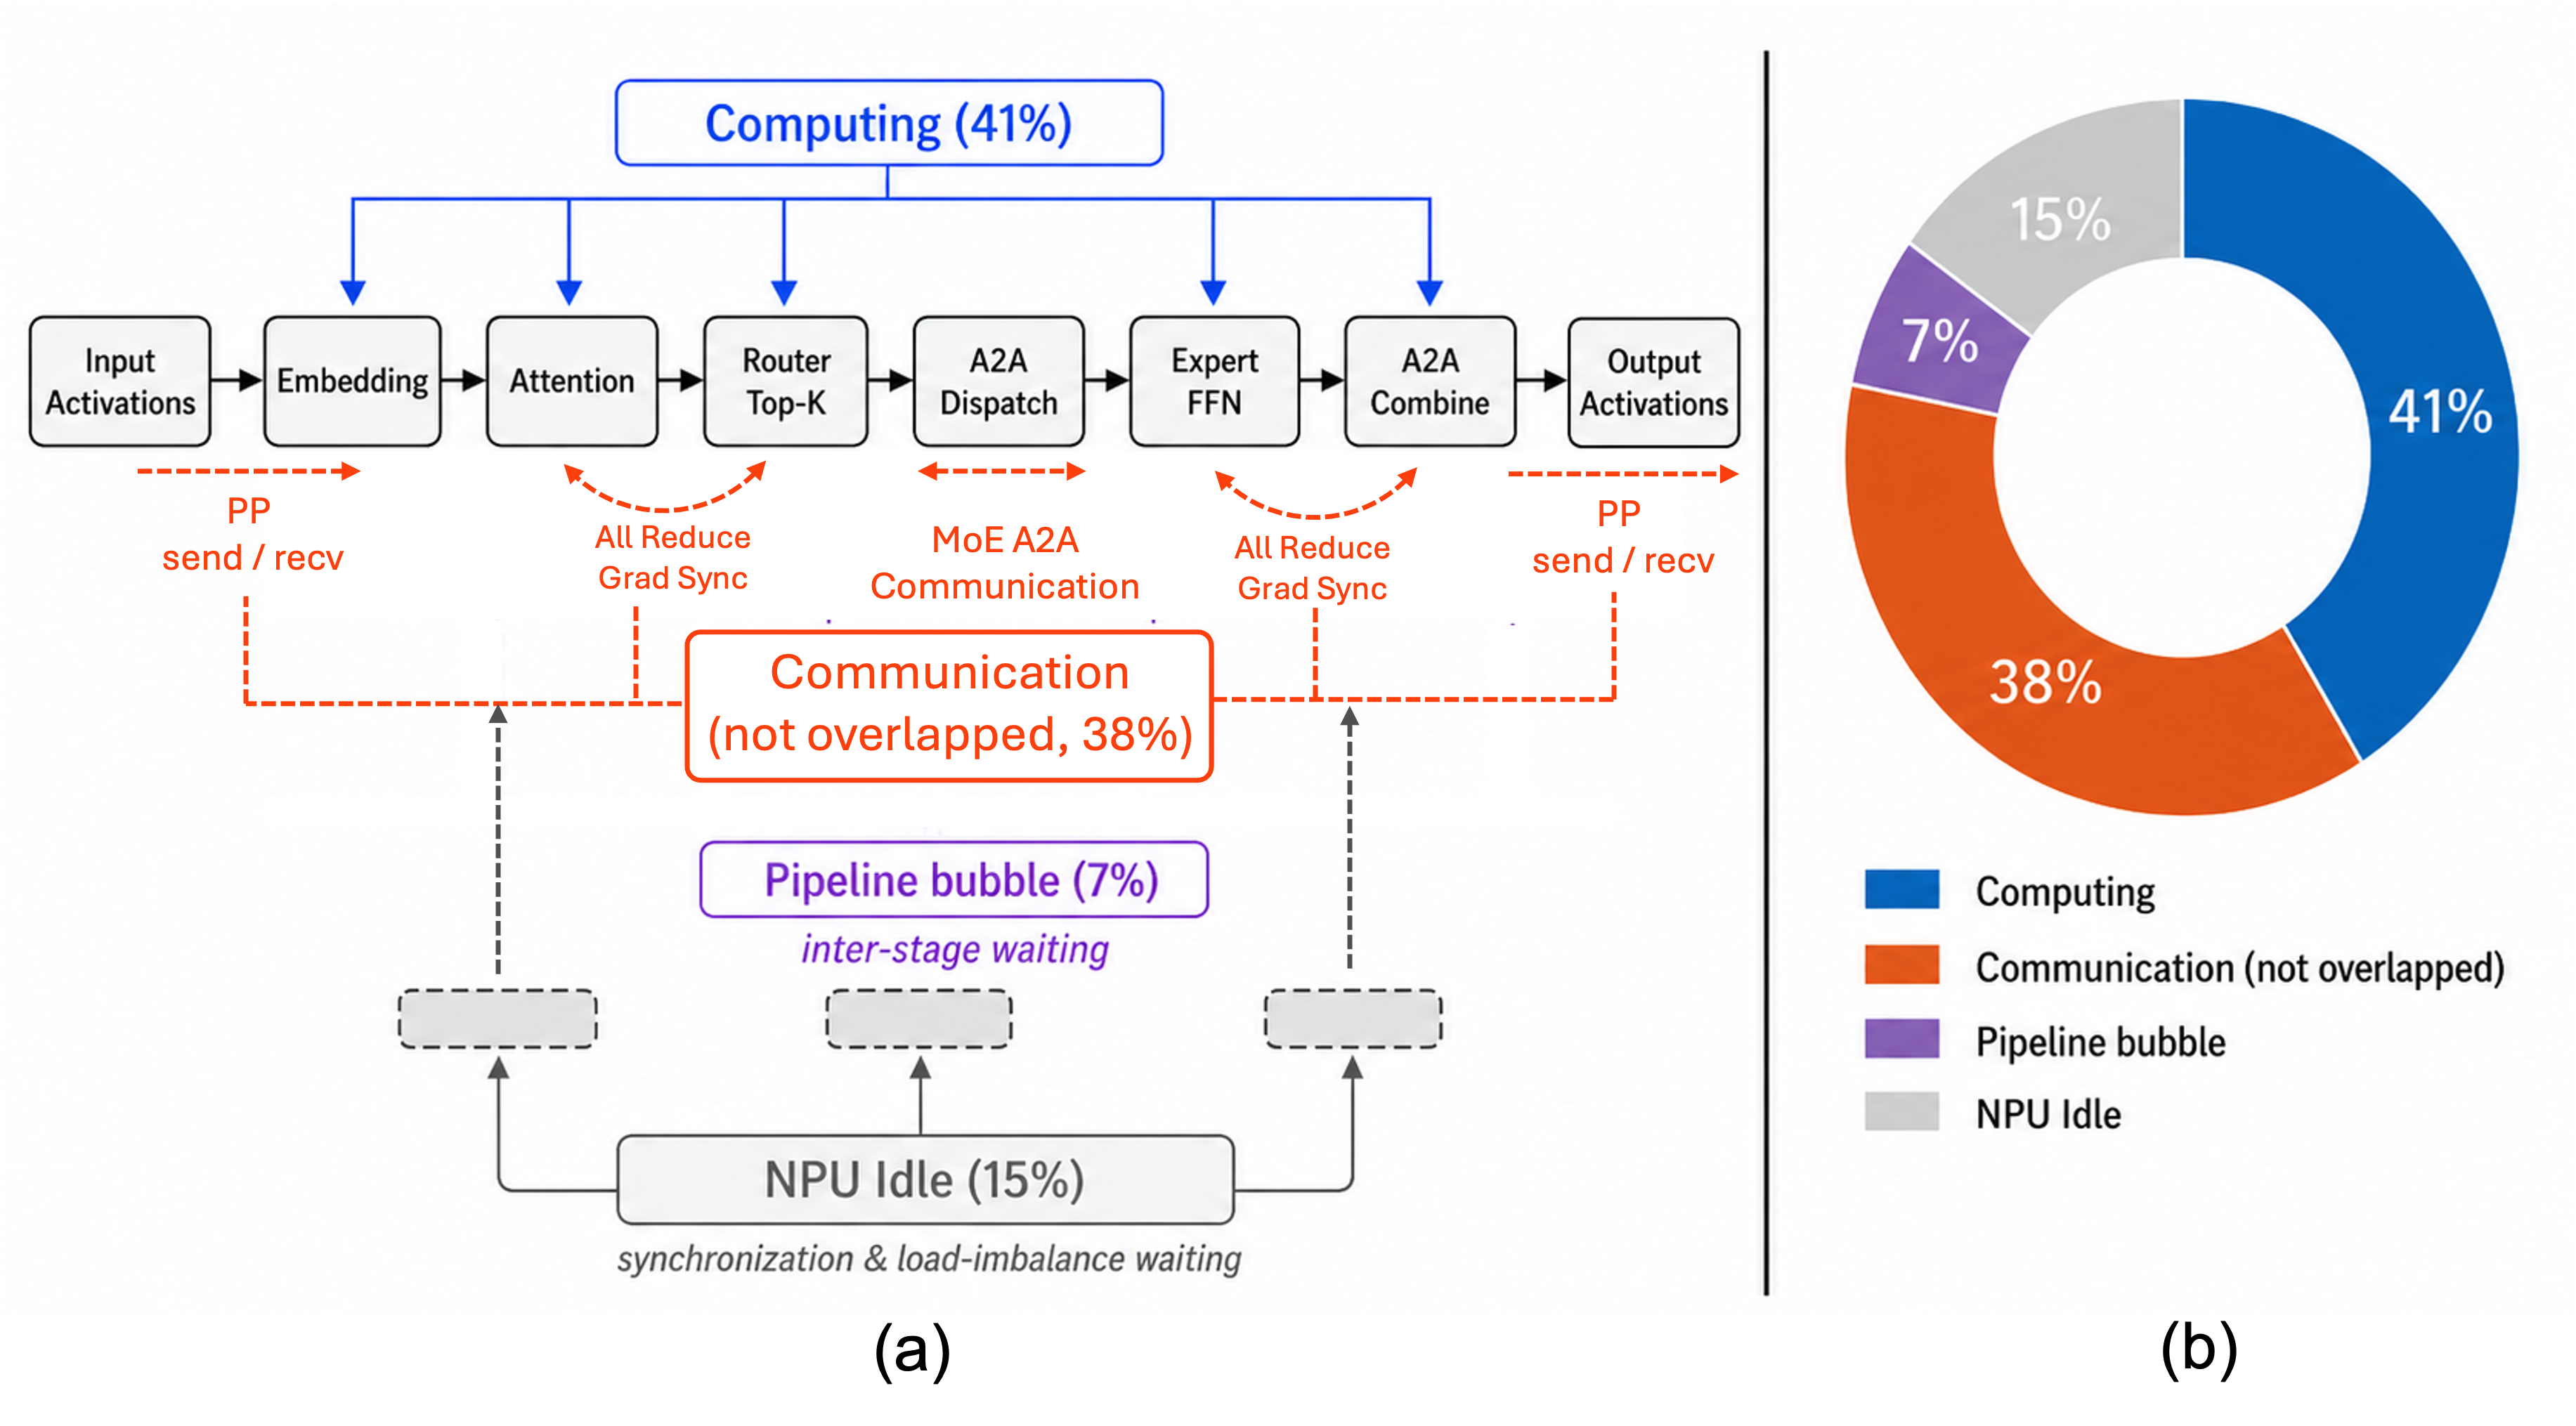
\includegraphics[width=0.9\linewidth]{figures/chapter2/ch2.1-fig_overview_v0.png}
    \caption{Latency breakdown of training trillion-parameter-class LLM model on Ascend SuperPOD NPU cluster. (a) Partition of latency in the end-to-end LLM training pipeline. (b) Averaged end-to-end latency breakdown, including computation, communication, and NPU idle bubble.}
    \label{fig:overview}
\end{figure}

\subsection{Bottlenecks of Training Trillion-parameter LLM on Ascend SuperPOD}\label{sec:bottleneck}
% We first profile the baseline to locate where training time is actually spent and to ground the design of the full-stack effort that follows. We collect a multi-rank profile of DeepSeek-V4-Pro pretraining on 256 Ascend 910C cards. The profile reveals that the inefficiency has two complementary faces. At the wall-clock level the step divides almost evenly between useful computation and communication that is not hidden behind it (Figure~\ref{fig:overview}); at the device level the busy kernel time divides between a small set of  operators and memory-bound kernels (Figure~\ref{fig:baseline_bottleneck}). We first analyze the exposed-communication regime that dominates the wall-clock view, then turn to the top bottleneck kernels and the fragmented memory-bound tail that dominate device time, and show how these regimes motivate the optimization strategies of this section.

\begin{table}[htp]
\centering
\caption{Communication latency breakdown by parallelism dimension in DeepSeek-V4-Pro training on Ascend SuperPOD, aggregated over the profiled ranks. Communication accounts for $52.2\%$ ($40.76$\,s) of the total device kernel time. Each collective/point-to-point primitive is attributed to the parallelism dimension that induces it: expert parallelism (\texttt{AllToAllV} token dispatch/combine), pipeline parallelism (point-to-point \texttt{Send}/\texttt{Receive} of inter-stage activations and gradients), and tensor/data parallelism (\texttt{AllReduce}, \texttt{AllGather}, and \texttt{ReduceScatter} for intra-layer reductions and sharded parameter/gradient exchange).}
\label{tab:comm_breakdown}
\resizebox{\textwidth}{!}{\begin{tabular}{llccc}
\toprule
\makecell[l]{Parallelism\\Dimension} & Communication Primitives & \makecell{Latency\\(s)} & \makecell{Share of\\Comm. (\%)} & \makecell{Share of\\Total (\%)} \\
\midrule
Tensor / Data (TP+DP) & \texttt{AllReduce}, \texttt{AllGather}, \texttt{ReduceScatter} & $19.71$ & $48.4$ & $25.2$ \\
Pipeline (PP)         & \texttt{Send}, \texttt{Receive} (P2P)                    & $14.95$ & $36.7$ & $19.2$ \\
Expert (EP)           & \texttt{AllToAllV} (MoE dispatch/combine)                & $5.91$  & $14.5$ & $7.6$  \\
Misc.                 & \texttt{Broadcast}, others                               & $0.18$  & $0.4$  & $0.2$  \\
% \midrule
% \textbf{Total}        & \textbf{All communication kernels}                       & $\mathbf{40.76}$ & $\mathbf{100.0}$ & $\mathbf{52.2}$ \\
\bottomrule
\end{tabular}}
\end{table}

\paragraph{Latency overhead induced by the non-overlapped communication.}

Given the scale of the target 1.6T-parameter model, we first adopt the baseline multi-dimensional parallelism to ensure training stability while keeping model states, activations, and optimizer states within the device memory budget, as summarized in Figure~\ref{fig:overview}.
However, training MoE models under such a multi-dimensional parallelism strategy inevitably introduces latency overhead across different partitions, due to frequent synchronization, collective communication, and data redistribution among parallel groups, as summarized in Table~\ref{tab:comm_breakdown}. 
% The profiling results indicates the fact that the communication contributes over half of the device kernel computation time, which requires collective optimization on both orchestration and model parallelism. 

The profiling results clearly indicate that the primary latency bottleneck is collecting partial results from the TP and DP partitions. Meanwhile, the send and receive latency introduced by the traditional 1F1B pipeline parallelism~(PP)~\citep{narayanan2021efficient} contributes a large portion toward the overall latency per training step. 
Benefiting from the high-speed interconnects of the Ascend SuperPOD, the communication overhead introduced by MoE remains minimal. 

% In our profile the exposed cost of these collectives has two scenario-specific causes. First, MoE execution is highly heterogeneous: attention, routing, dispatch, expert FFNs, and combine differ in compute and communication intensity, and token routing shifts the expert load from step to step, so the overlap window is neither uniform nor stable, and an otherwise overlap-friendly collective becomes exposed whenever its producer stage finishes late or its compute window is shortened by sparse activation and load imbalance. Second, on Ascend the measured communication cost is dominated not by inter-device transfer but by communication-adjacent overhead such as tensor packing, layout transformation, stream synchronization, and launch ordering; the profile accordingly shows negligible transit time but substantial barrier waiting, indicating that the bottleneck is scheduling rather than bandwidth.

Based on this analysis, the latency of one training step can be decomposed into four major components:
\[
T_{\mathrm{step}} =
T_{\mathrm{comp}} +
T_{\mathrm{comm}}^{\mathrm{non-overlapped}} +
T_{\mathrm{bubble}} +
T_{\mathrm{idle}},
\]
where $T_{\mathrm{comp}}$ corresponds to useful dense and sparse model computation, $T_{\mathrm{comm}}^{\mathrm{exposed}}$ denotes communication that is not fully hidden by computation, $T_{\mathrm{bubble}}$ captures inter-stage waiting caused by pipeline parallelism, and $T_{\mathrm{idle}}$ represents device-side stalls caused by synchronization, load imbalance, and unresolved runtime dependencies.

In addition to the absolute latency introduced by the parallelism-induced communication~(\texttt{hcom\_} kernels), 
the imbalanced computation workload between different PP stages further introduces a latency bubble throughout the training process. 
As depicted in Figure~\ref{fig:overview}(b), the computation bubble exists uniformly across different stages of pipeline parallelism. 

% \begin{figure}[h]
% \centering
% \includegraphics[width=\textwidth]{figures/chapter2/ch2.1-baseline_bottleneck.png}
% \caption{Baseline bottleneck anatomy of DeepSeek-V4-Pro training on 256 Ascend 910C NPUs, complementary to the wall-clock latency breakdown of Figure~\ref{fig:overview}. (a)~Decomposition of step time into computing, exposed (non-overlapped) communication, and pipeline bubble. (b)~Share of kernel launches versus share of device time for the large cube kernels, the vector tail, and communication kernels, contrasting cost concentration with launch fragmentation. (c)~Duration-weighted pipeline occupancy of vector-core kernels, split into vector-compute pipes and MTE2/MTE3 memory-movement pipes. (d)~Share of kernel launches versus share of device time across kernel-duration buckets, comparing the many small kernels with the few large ones.}
% \label{fig:baseline_bottleneck}
% \end{figure}

% Figure~\ref{fig:overview} decomposes the step into computation, exposed communication, pipeline bubbles, and NPU idle, and the way this budget is split is itself the central finding. The most telling feature is that exposed communication is nearly as large as useful computation: on a well-provisioned interconnect the collectives are not bandwidth-starved but simply fail to hide behind compute, so almost as much of the step is spent waiting on communication as doing model arithmetic. This near parity is the signature of a scheduling-bound rather than compute-bound regime, where the ceiling is set by how work is overlapped and ordered, not by raw FLOPs, so buying faster cores would leave most of the step untouched. The bubble and idle slices reinforce the same diagnosis from the opposite direction. They are pure stalls that no kernel-level speedup can remove, and their true weight is understated here because stage stalls that spill into send/receive are billed as communication rather than as explicit bubbles, so the real pipeline- and synchronization-related overhead is somewhat larger than the idle and bubble slices alone suggest. Crucially, the idle time clusters around exactly the attention, dispatch, and combine regions where MoE routing makes the per-step load imbalanced and data-dependent, which is why it cannot be scheduled away statically and instead motivates the dynamic overlap and load-balancing mechanisms developed below. Taken together, the breakdown says that the dominant loss lives in the seams between operations rather than inside them, and it is this exposed-communication-plus-stall majority, not the computation slice, that the remainder of this section sets out to reclaim.

% Table~\ref{tab:comm_breakdown} breaks the exposed communication down by parallelism axis. Pipeline send/receive dominates the head stage (71\%) and gradient all-reduce dominates the tail (61\%), while expert and tensor-parallel traffic stay below 20\% combined; transit time is negligible at every stage, confirming the cost is synchronization wait rather than bandwidth.

% \begin{table}[t]
%   \centering
%   \caption{Exposed communication per step, by parallelism axis and pipeline stage
%   (seconds, with share of that stage's exposed communication). Transit time is
%   negligible throughout: the cost is synchronization wait, not bandwidth.}
%   \label{tab:comm_breakdown}
%   \begin{tabular}{lccc}
%     \toprule
%     Communication & Stage 0~(Head) & Stage 4~(Middle) & Stage 7~(Tail) \\
%     \midrule
%     PP send/recv      & 8.6 (71\%) & 3.8 (33\%) & 2.5 (23\%) \\
%     DP all-reduce     & 1.6 (13\%) & 5.6 (49\%) & 6.8 (61\%) \\
%     EP all-to-all     & 0.8 (7\%)  & 1.0 (9\%)  & 0.7 (7\%)  \\
%     TP all-gather/RS  & 1.1 (9\%)  & 1.1 (9\%)  & 1.0 (9\%)  \\
%     \midrule
%     Total exposed     & 12.1       & 11.4       & 11.1       \\
%     \bottomrule
%   \end{tabular}
% \end{table}


\paragraph{Dominant latency from model-specific kernels.}
Taking a closer look at the detailed kernel execution time, we observe that the latency of computation is dominated by a small set of architecture-specific kernels.
In particular, DeepSeek-V4 introduces the hierarchical sparse attention with heavy execution time on Ascend NPUs.
As depicted in Table~\ref{tab:kernel_bottleneck}, the backward kernel of sparse attention constitutes one of the most significant bottlenecks among all AscendC operators, where the total execution time is even comparable to the generic matrix multiplication operators. Throughout this analysis, an operator's Task-Duration share is its summed core-busy time---the per-kernel AI-Core or vector-core execution time---normalized over the $206{,}503$ compute kernels of one step after excluding communication and AI-CPU entries, with invocation count and average per-call duration listed alongside to expose the fragmented, long-tailed operators.

Concretely, the sparse-attention family contributes roughly a quarter of the non-communication kernel time, exceeding the combined share of the dense \texttt{MatMulV3} and MoE \texttt{GroupedMatmul} operators.
This concentration is intrinsic to the model architecture rather than an artifact of a particular layer configuration: the lightning indexer that selects the sparse key--value context and the shared-KV attention that consumes it are invoked in every attention block~\citep{deepseekai2026deepseekv4highlyefficientmilliontoken}, so their cost scales directly with the depth of the network.

The profiling results also make it clear \emph{why} these kernels are slow, and their bottlenecks differ fundamentally from those of matrix-multiplication operators.
The dense \texttt{MatMulV3} and MoE \texttt{GroupedMatmul} kernels are compute-bound and run on the CUBE core near saturation (over $90\%$ utilization), converting their latency into useful matrix throughput. Among these, \texttt{GroupedMatmul} is genuinely MAC-dominated, whereas \texttt{MatMulV3} is operand-load-bound, its MTE2 load share ($96.3\%$) far exceeding its MAC share ($52.5\%$).
The sparse-attention kernels do the opposite: their compute engines sit largely idle (vector-compute pipeline ratio of about $9.5\%$), and their runtime is instead spent moving key--value tiles through the local buffers and executing the scalar index and gather/scatter logic needed to assemble the sparse attention pattern.
In other words, these operators are memory- and control-bound rather than compute-bound---they occupy the top of the latency profile not because they perform heavy computation, but because their data-dependent, irregular access pattern keeps the hardware's matrix engine starved.

Motivated by these findings, this work proposes \textbf{AuraKernel}, an end-to-end AscendC kernel optimization agent that automatically restructures the large, memory- and control-bound AscendC kernels, as presented in Section~\ref{sec:kernel_agent}. 
% the shared-key-value sparse-attention backward, grouped expert (MoE) multiplication, dense matrix multiplication, and the sparse lightning-indexer gradient. 
% As Figure~\ref{fig:baseline_bottleneck}(b) makes explicit, these large cube kernels are only $7.5\%$ of all kernel launches yet account for $48.5\%$ of device time; their individual duration shares and pipeline counters are reported in Table~\ref{tab:kernel_bottleneck}. Because their cost is intrinsic to the model architecture and already maps well onto the Ascend Cube engine, the remaining headroom lies inside the kernel body---tiling, memory layout, pipeline overlap, and instruction scheduling---rather than in eliminating the kernels themselves. This concentrated, compute-bound head is the target of the profiling-in-the-loop kernel-optimization agent AuraKernel (Section~\ref{sec:kernel_opt}).

\begin{table}[htp]
\centering
\caption{Representative top operators in DeepSeek-V4-Pro training on Ascend 910C at global batch size $1024$, ranked by Task-Duration share. Cube rows report AIC counters (MAC, MTE2, Fixpipe store, cube utilization) and vector rows AIV counters (vector compute, MTE2, MTE3, scalar utilization); the store column is therefore Fixpipe for cube rows and MTE3 for vector rows. The final row aggregates the remaining $92$ operator types. Share definition and profiling scope are given in the text.}
\label{tab:kernel_bottleneck}
\resizebox{\textwidth}{!}{%
\begin{tabular}{clcrrcccc}
	\toprule
	Rank & Operator & \makecell{Task Dur.\\Share} & Calls & \makecell{Avg\\($\mu$s)} & \makecell{Compute\\(MAC/Vec)} & \makecell{MTE2\\Load} & \makecell{Store\\(MTE3/Fix)} & \makecell{Cube/Scalar\\Util.} \\
	\midrule
	1 & \texttt{SparseAttnSharedkvGrad} (sparse-attn bwd) & $16.86\%$ & $224$    & $27{,}593$ & $9.5\%$  & $21.3\%$ & $34.2\%$ & $15.1\%$ \\
	2 & \texttt{MatMulV3}                                 & $12.77\%$ & $5{,}600$ & $836$      & $52.5\%$ & $96.3\%$ & $21.8\%$ & $85.4\%$ \\
	3 & \texttt{GroupedMatmul} (MoE experts)              & $9.50\%$  & $1{,}344$ & $2{,}592$  & $86.8\%$ & $96.2\%$ & $11.4\%$ & $95.4\%$ \\
	4 & \texttt{Cast}                                     & $6.02\%$  & $40{,}063$ & $55$      & $5.7\%$  & $89.7\%$ & $59.9\%$ & $1.7\%$ \\
	5 & \texttt{SparseLightningIndexerGradKLLoss}         & $5.52\%$  & $96$    & $21{,}082$ & $5.5\%$  & $7.9\%$  & $5.4\%$  & $96.0\%$ \\
	6 & \texttt{Add}                                      & $5.40\%$  & $16{,}579$ & $119$    & $14.0\%$ & $93.4\%$ & $23.0\%$ & $2.3\%$ \\
	7 & \texttt{GmmAddKernel} (MoE weight-grad)           & $4.72\%$  & $448$   & $3{,}859$  & $58.8\%$ & $89.4\%$ & $24.0\%$ & $95.8\%$ \\
	8 & \texttt{PpMatmulAccumAtomicKernel}                & $3.26\%$  & $896$   & $1{,}335$  & $63.5\%$ & $95.6\%$ & $9.2\%$  & $95.1\%$ \\
	9 & \texttt{BatchMatMulV2}                            & $3.06\%$  & $896$   & $1{,}253$  & $64.1\%$ & $98.7\%$ & $12.1\%$ & $94.3\%$ \\
	\midrule
	\multicolumn{2}{l}{Long tail ($92$ remaining operator types)} & $32.88\%$ & $140{,}357$ & $\approx 86$ & \multicolumn{4}{l}{predominantly small, memory-bound vector \& copy kernels} \\
	\bottomrule
	\end{tabular}}
\end{table}
\paragraph{The long tail of fragmented, memory-bound kernels.}
In addition to the top-ranked bottleneck kernels with insufficient utilization on Ascend NPUs, we observe a long tail of small kernel invocations that consistently appear in each training step, as shown in Table~\ref{tab:kernel_bottleneck}. While each individual kernel contributes only a short execution time, these fragmented kernel calls collectively account for a substantial fraction of the overall computation time.

A closer inspection shows that these long-tailed kernels are primarily element-wise and data-movement operators, such as \texttt{Cast} and \texttt{Add}, together with tensor copy and reshape operations. These operators are invoked frequently, yet each typically completes within only tens of microseconds. Unlike cube-bound matrix-multiplication kernels, these fragmented operators execute almost entirely on the vector core, where the load/store pipelines are significantly more active than the vector-compute pipeline. As shown in Table~\ref{tab:kernel_bottleneck}, the \texttt{Cast} operator alone contributes $5.7\%$ of the total computation time. However, the vector-compute utilization of \texttt{Cast} remains nearly idle~(computing core utilization $\approx 1.7\%$), whereas the memory-transfer pipelines remain heavily occupied, with AIV MTE2/MTE3 at $89.7\% / 59.9\%$. This imbalance indicates that such operators are primarily memory-bound and are natural candidates for fusion with neighboring kernels.

Overall, kernel fragmentation further degrades system-level efficiency due to the newly proposed model architecture~(e.g., mHC~\citep{mhc2025} hyper-connections) in the DeepSeek-V4 model. 
These kernels have very short execution times, where the fixed costs of kernel launch and scheduling can no longer be effectively amortized. 
Furthermore, repeated round trips to memory introduce redundant data movement and inflate the aggregate overhead. 
As a result, the collective footprint of these fragmented, memory-bound operators is far from negligible, motivating a consolidation strategy based on dedicated kernel fusion to suppress launch overhead and eliminate redundant memory traffic, as presented in Section~\ref{sec:kernel_fusion}. 


% The remaining device time is spread across a long tail of vector-core kernels that constitute $78\%$ of all launches but only about a third ($33\%$) of device time (Figure~\ref{fig:baseline_bottleneck}(b)). Two further profiling views explain why this tail is doubly wasteful. First, it is \emph{fragmented}: binning kernels by duration (Figure~\ref{fig:baseline_bottleneck}(d)), sub-$20\,\mu$s kernels are $61\%$ of all launches but only about $4\%$ of device time, whereas the few kernels above $50\,\mu$s carry $92\%$ of it, so the tail pays a large, recurring launch-and-scheduling overhead for very little useful work. Second, it is \emph{memory-bound}: aggregated over all vector-core kernels, the duration-weighted vector-compute pipe occupancy is only $\approx 0.15$, while the MTE2 (load) and MTE3 (store) memory-movement pipes reach $\approx 0.60$ and $\approx 0.36$ (Figure~\ref{fig:baseline_bottleneck}(c)), so most vector-kernel time is spent moving data between global memory and the on-chip buffers rather than computing. The tail is dominated by framework-emitted, autograd-expanded chains around the model arithmetic---elementwise \texttt{Add}, \texttt{Cast}, and \texttt{Mul}; buffer and layout kernels such as \texttt{ViewCopy} and \texttt{Transpose}; weight-free RMS normalization; and the limited-SwiGLU clamp and concatenation---each individually small but collectively large (their durations and pipeline counters are itemized in Table~\ref{tab:kernel_bottleneck}). Because the cost is paid in launch count, tensor materialization, and data movement rather than arithmetic, the remedy is not faster math but fewer, larger, hardware-aligned kernels: recovering the high-level operation and re-expressing it as a Unified-Buffer-resident AscendC kernel that keeps intermediates on chip. This is the proactive operator-chain fusion of Section~\ref{sec:kernel_fusion}.

% In summary, the baseline profile partitions the inefficiency into three regimes: exposed communication on the wall-clock critical path, a concentrated compute-bound head on the device, and a fragmented, memory-bound tail on the device. None of these is removable by faster hardware alone, and each demands a different, hardware-aware remedy. Reducing step time therefore requires coordinated full-stack optimization, and the three regimes map directly onto the strategies developed in the remainder of this section: Ascend-friendly multi-dimensional parallelism with efficient token dispatch and computation--communication overlap to hide exposed communication (Section~\ref{sec:infra_framework}), AuraKernel profiling-in-the-loop kernel tuning for the compute-bound head (Section~\ref{sec:kernel_opt}), and proactive operator-chain fusion that re-maps the memory-bound tail onto the Ascend memory hierarchy (Section~\ref{sec:kernel_fusion}).


% tentative title
\subsection{Optimizing Trillion-parameter LLM Training System on Ascend SuperPOD }\label{sec:infra_framework}

\begin{figure}[t]
  \centering
  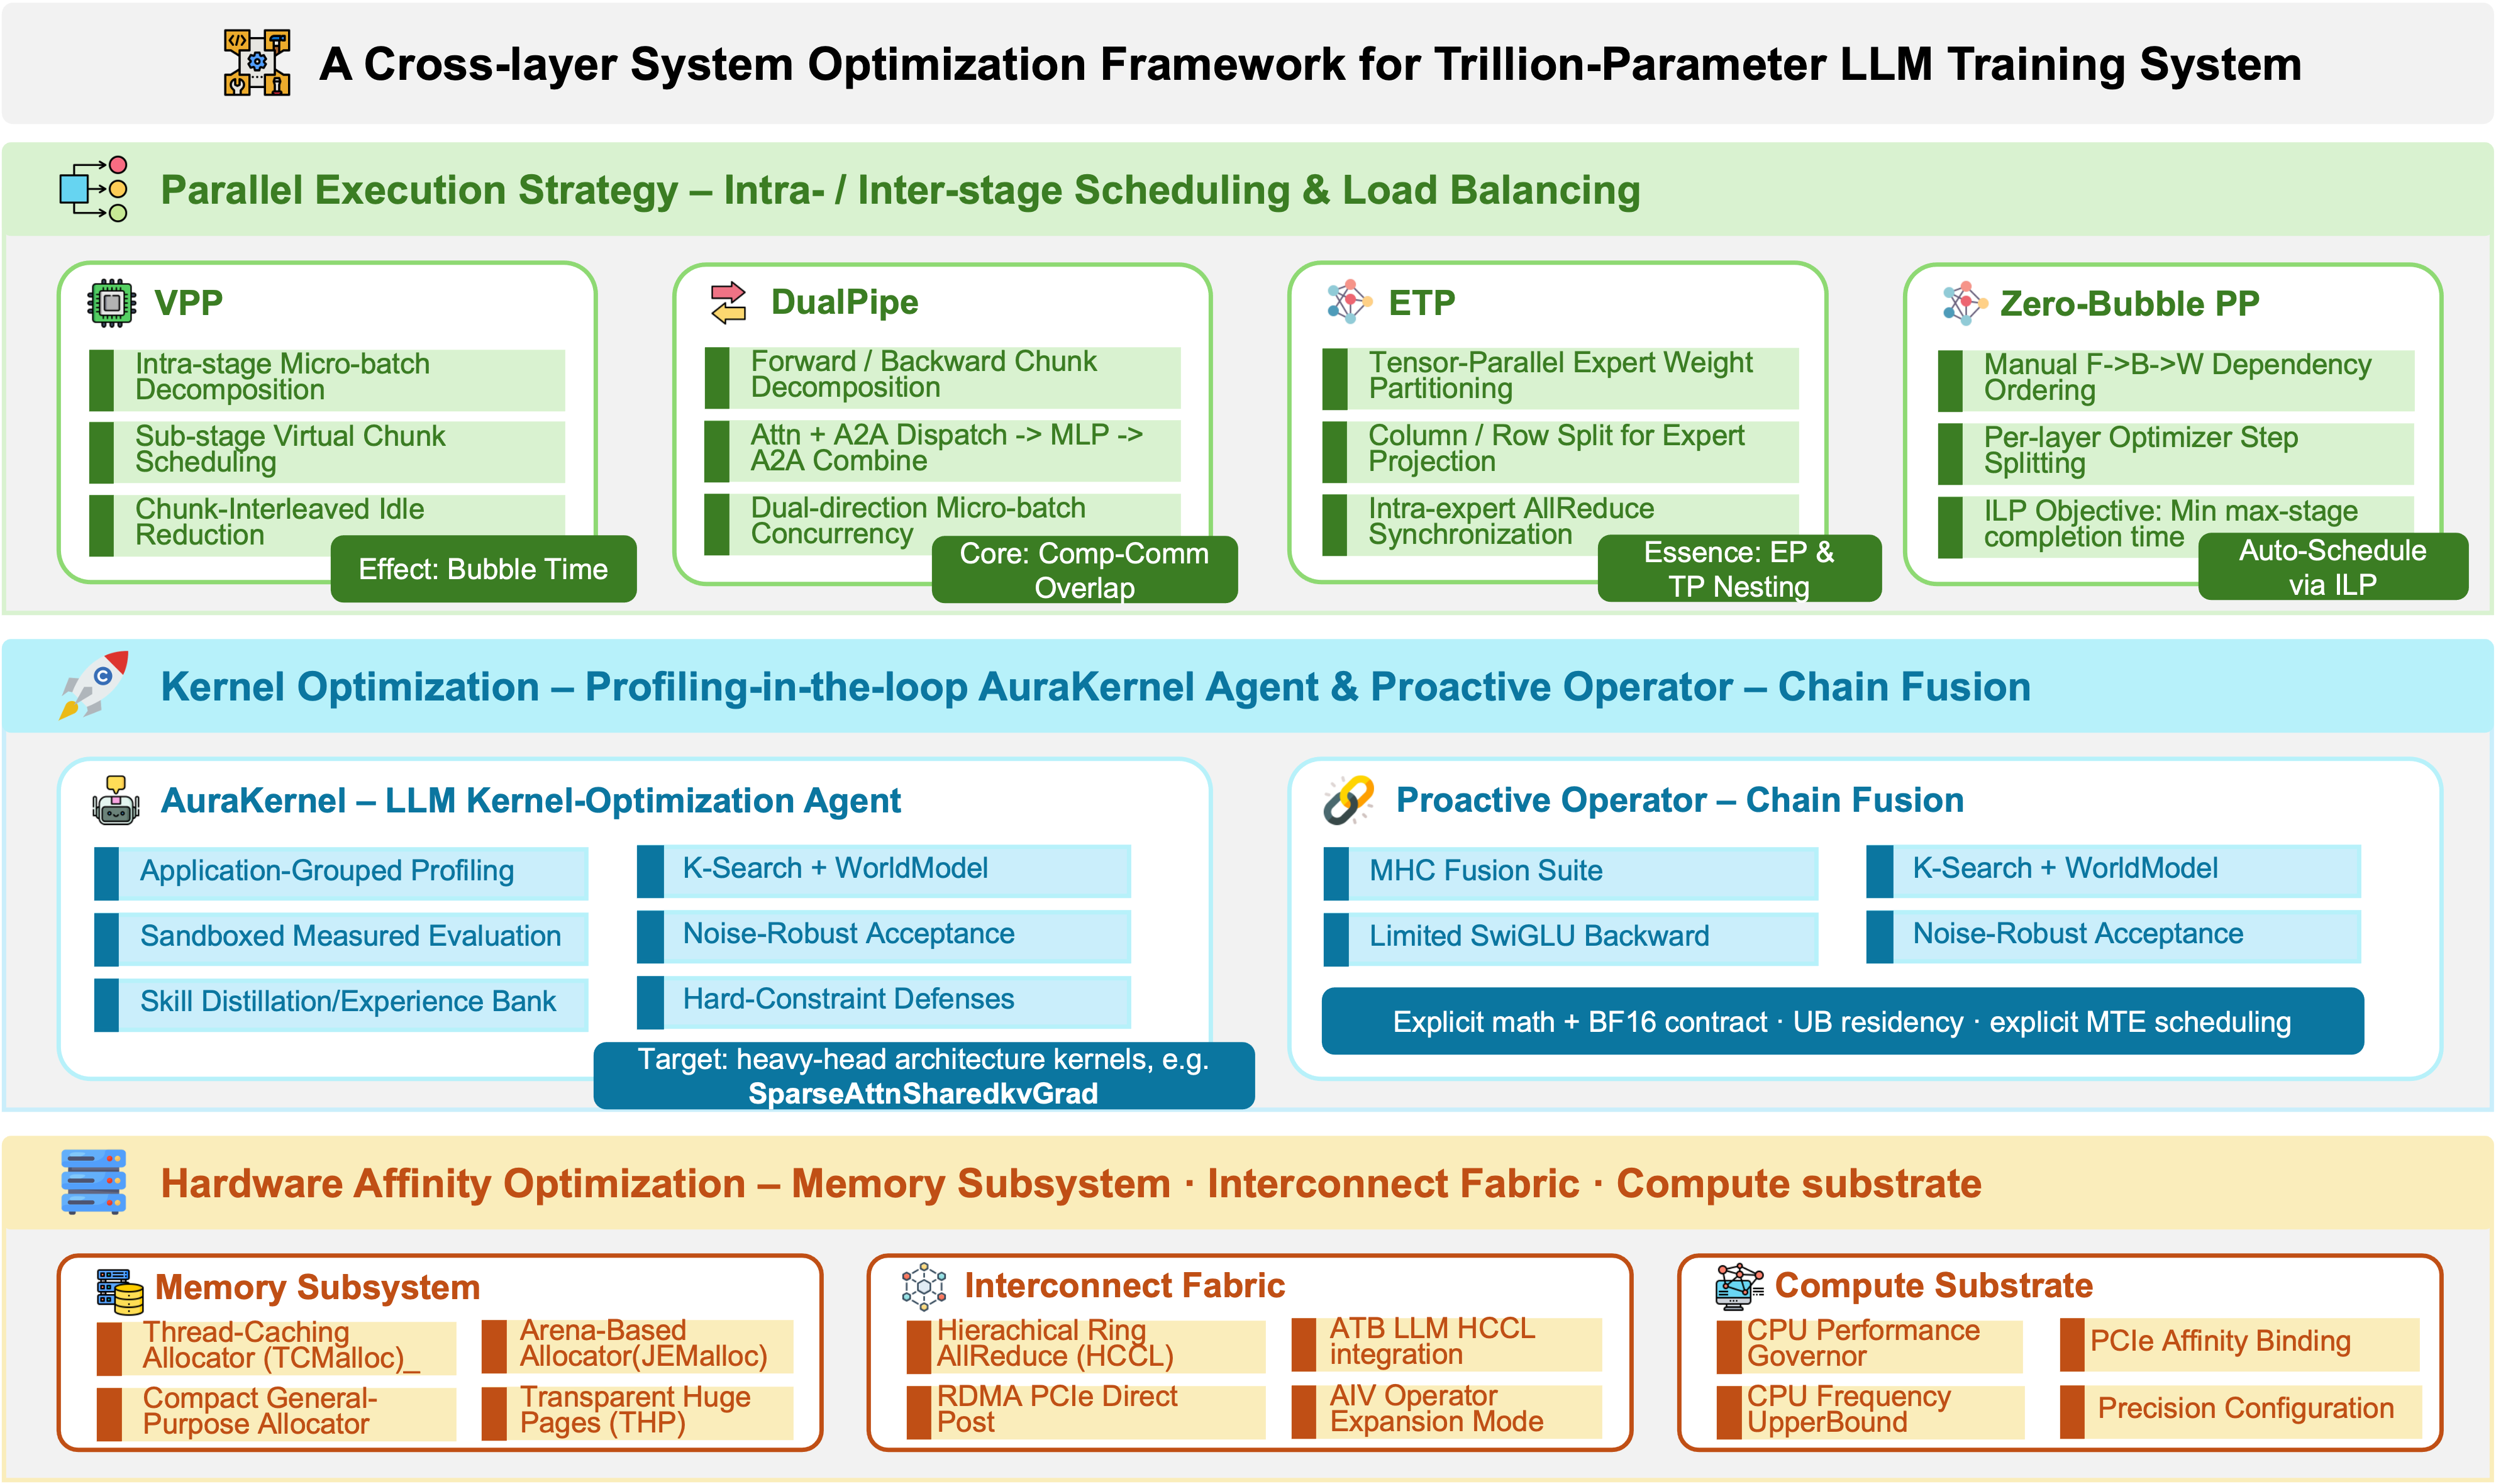
\includegraphics[width=\textwidth]{figures/chapter2/ch2.2-train_framework.png}
  \caption{Overview of the proposed full-stack optimization framework, which includes three cooperating layers: parallel execution strategy, kernel optimization, and hardware-affinity tuning.}
  \label{fig:train_framework}
\end{figure}

Motivated by the bottleneck analysis in Section~\ref{sec:bottleneck}, we optimize end-to-end training performance through a hierarchical three-layer strategy: \circled{1} Optimal computation-communication orchestration via optimized training parallelism, \circled{2} Agent-driven optimization of top-ranked bottleneck kernels with AuraKernel, and \circled{3} Full-stack operator fusion to eliminate fragmented kernel overhead. The overall framework is illustrated in Figure~\ref{fig:train_framework}. 
% (AuraKernel together with operator-chain fusion) that addresses the top bottleneck kernels and fragmented memory-bound tail, and hardware-affinity tuning of the Ascend memory, interconnect, and compute substrates.



% The latency analysis of Section~\ref{sec:bottleneck} shows that the baseline step is co-limited by exposed communication, pipeline bubbles, and the memory pressure that forces activation recomputation. Parallel-strategy optimization attacks all three at once: rather than changing what is computed, it reshapes how the multi-dimensional parallelism is scheduled so that the unavoidable stalls of distributed execution are hidden behind independent work, under a fixed HBM budget. The top layer of Figure~\ref{fig:train_framework} groups these techniques into intra-/inter-stage pipeline scheduling and load balancing, an Ascend-centric MoE token dispatcher that overlaps expert communication with computation, and a swap-based optimizer that relieves device memory. We outline the scheduling techniques and then analyze the dispatcher and the optimizer in depth. The principle is to convert serialized dependencies into pipelined concurrency on independent streams.

\paragraph{Load-balanced pipeline scheduling and expert--tensor parallelism (ETP).}
\label{subsec:etp}
As discussed in Section~\ref{sec:bottleneck}, reducing the exposed communication overhead introduced by tensor parallelism~(TP) is a primary optimization target. Due to the limited memory capacity of each Ascend 910C NPU~(64GB), a naive parallelization strategy requires a relatively high TP degree, such as TP=4, to fit the model states and activations within the device memory budget. However, this also increases the frequency and cost of TP collectives.

Following the Parallel Folding strategy in Megatron-LM~\citep{shoeybi2019megatron}, we enable expert-tensor parallelism~(ETP) for MoE layers while keeping the pipeline parallelism~(PP) configuration fixed. This decouples the parallelism choices between attention and MoE modules: attention layers can adopt a lower TP degree~(TP=2) to reduce communication overhead and improve GEMM efficiency on large dense matrices, while MoE layers use ETP=1 to preserve the full expert width and avoid further fragmenting expert computation. The resulting dispatch and execution strategy is illustrated in Figure~\ref{fig:etp-dispatcher}.

\paragraph{Virtual Pipeline Parallelism~(VPP) vs. DualPipeV.}
For the pipeline dimension (with a pipeline degree of $8$), we adopt VPP ~\citep{narayanan2021efficient} rather than the bidirectional DualPipeV ~\citep{qi2025dual,deepseekai2025deepseekv3technicalreport} schedule, for two complementary reasons grounded in our profiling.
First, DualPipeV~\citep{qi2025dual,deepseekai2025deepseekv3technicalreport} is memory-prohibitive at this scale: to sustain its bidirectional overlap, each device must retain two model chunks, roughly doubling the resident parameters and gradients, together with a larger population of in-flight micro-batch activations.
Our traces show that, even under the more memory-frugal VPP schedule, the peak reserved device memory already reaches $51.7$--$54.6$\,GB per NPU across the profiled ranks, leaving only a narrow margin from the per-device HBM budget; the additional residency demanded by DualPipeV would readily overshoot this limit, forcing a smaller micro-batch size or heavier recomputation that erodes its purported efficiency gains.
Second, and more fundamentally, DualPipeV's headline capability, overlapping the expert-parallel all-to-all (MoE dispatch/combine) with computation, targets a cost that is simply not our bottleneck.
In our profiling, the all-to-all accounts for only $14.5\%$ of communication time, whereas the communication cost is dominated by pipeline point-to-point transfers ($36.7\%$ of communication, driven largely by receive-side stalls that reflect stage-level bubbles and load imbalance) and by tensor-/data-parallel \texttt{AllReduce} ($48.4\%$ of communication).

The pipeline-bubble is precisely what VPP mitigates by introducing fine-grained interleaving of virtual stages.
Consequently, DualPipeV would incur a substantial memory penalty in exchange for accelerating a component that contributes marginally to our end-to-end latency, whereas VPP suppresses the dominant pipeline bubbles while keeping the per-device footprint within the hardware budget and training stability. 
We will further investigate the optimal pipeline parallelism strategy in the near future. 

% The first lever targets the pipeline bubble $T_{\mathrm{bubble}}$ and part of the exposed communication $T_{\mathrm{comm}}^{\mathrm{exposed}}$ identified in Section~\ref{sec:bottleneck}. On the Ascend super-pod the deep pipeline and the step-to-step shift of MoE expert load make these stalls both large and uneven, so the remedy is to fill each stage's idle window with independent work rather than to shorten any single computation. Virtual pipeline parallelism (VPP) splits each stage into finer virtual chunks, lowering the bubble ratio from $O(1/m)$ to $O(1/(mv))$ for $m$ micro-batches and $v$ virtual chunks, i.e. finer chunking leaves a smaller fraction of the pipeline idle. A bidirectional dual-stream pipeline (DualPipe) runs forward and backward micro-batches in opposite directions and interleaves their attention, all-to-all dispatch, MLP, and all-to-all combine, so the routing communication of one direction is concealed behind the computation of the other. Zero-bubble scheduling further lifts the weight-gradient step off the critical path and reorders it into the remaining gaps. Together these shrink the inter-stage waiting and push part of the exposed routing traffic behind useful computation.

% At the trillion-parameter scale, individual experts can be too large to replicate on a single die, so expert parallelism alone cannot keep shards balanced without inflating the expert-parallel degree. Expert--tensor parallelism (ETP) nests tensor parallelism inside expert parallelism, so each rank stores and computes only an $H/\mathrm{ETP}$ slice of every expert. The reason we adopt it here is memory: partitioning the expert along the hidden dimension keeps activations sharded on both sides of the grouped-GEMM and balances the per-rank memory and compute footprint, at the cost of extra intra-expert collectives (an all-gather before and a reduce-scatter after the GEMM) rather than a single post-GEMM all-reduce. Figure~\ref{fig:etp-dispatcher} shows the resulting dispatcher communication for an ETP2--EP2 example.

\begin{figure}[t]
\centering
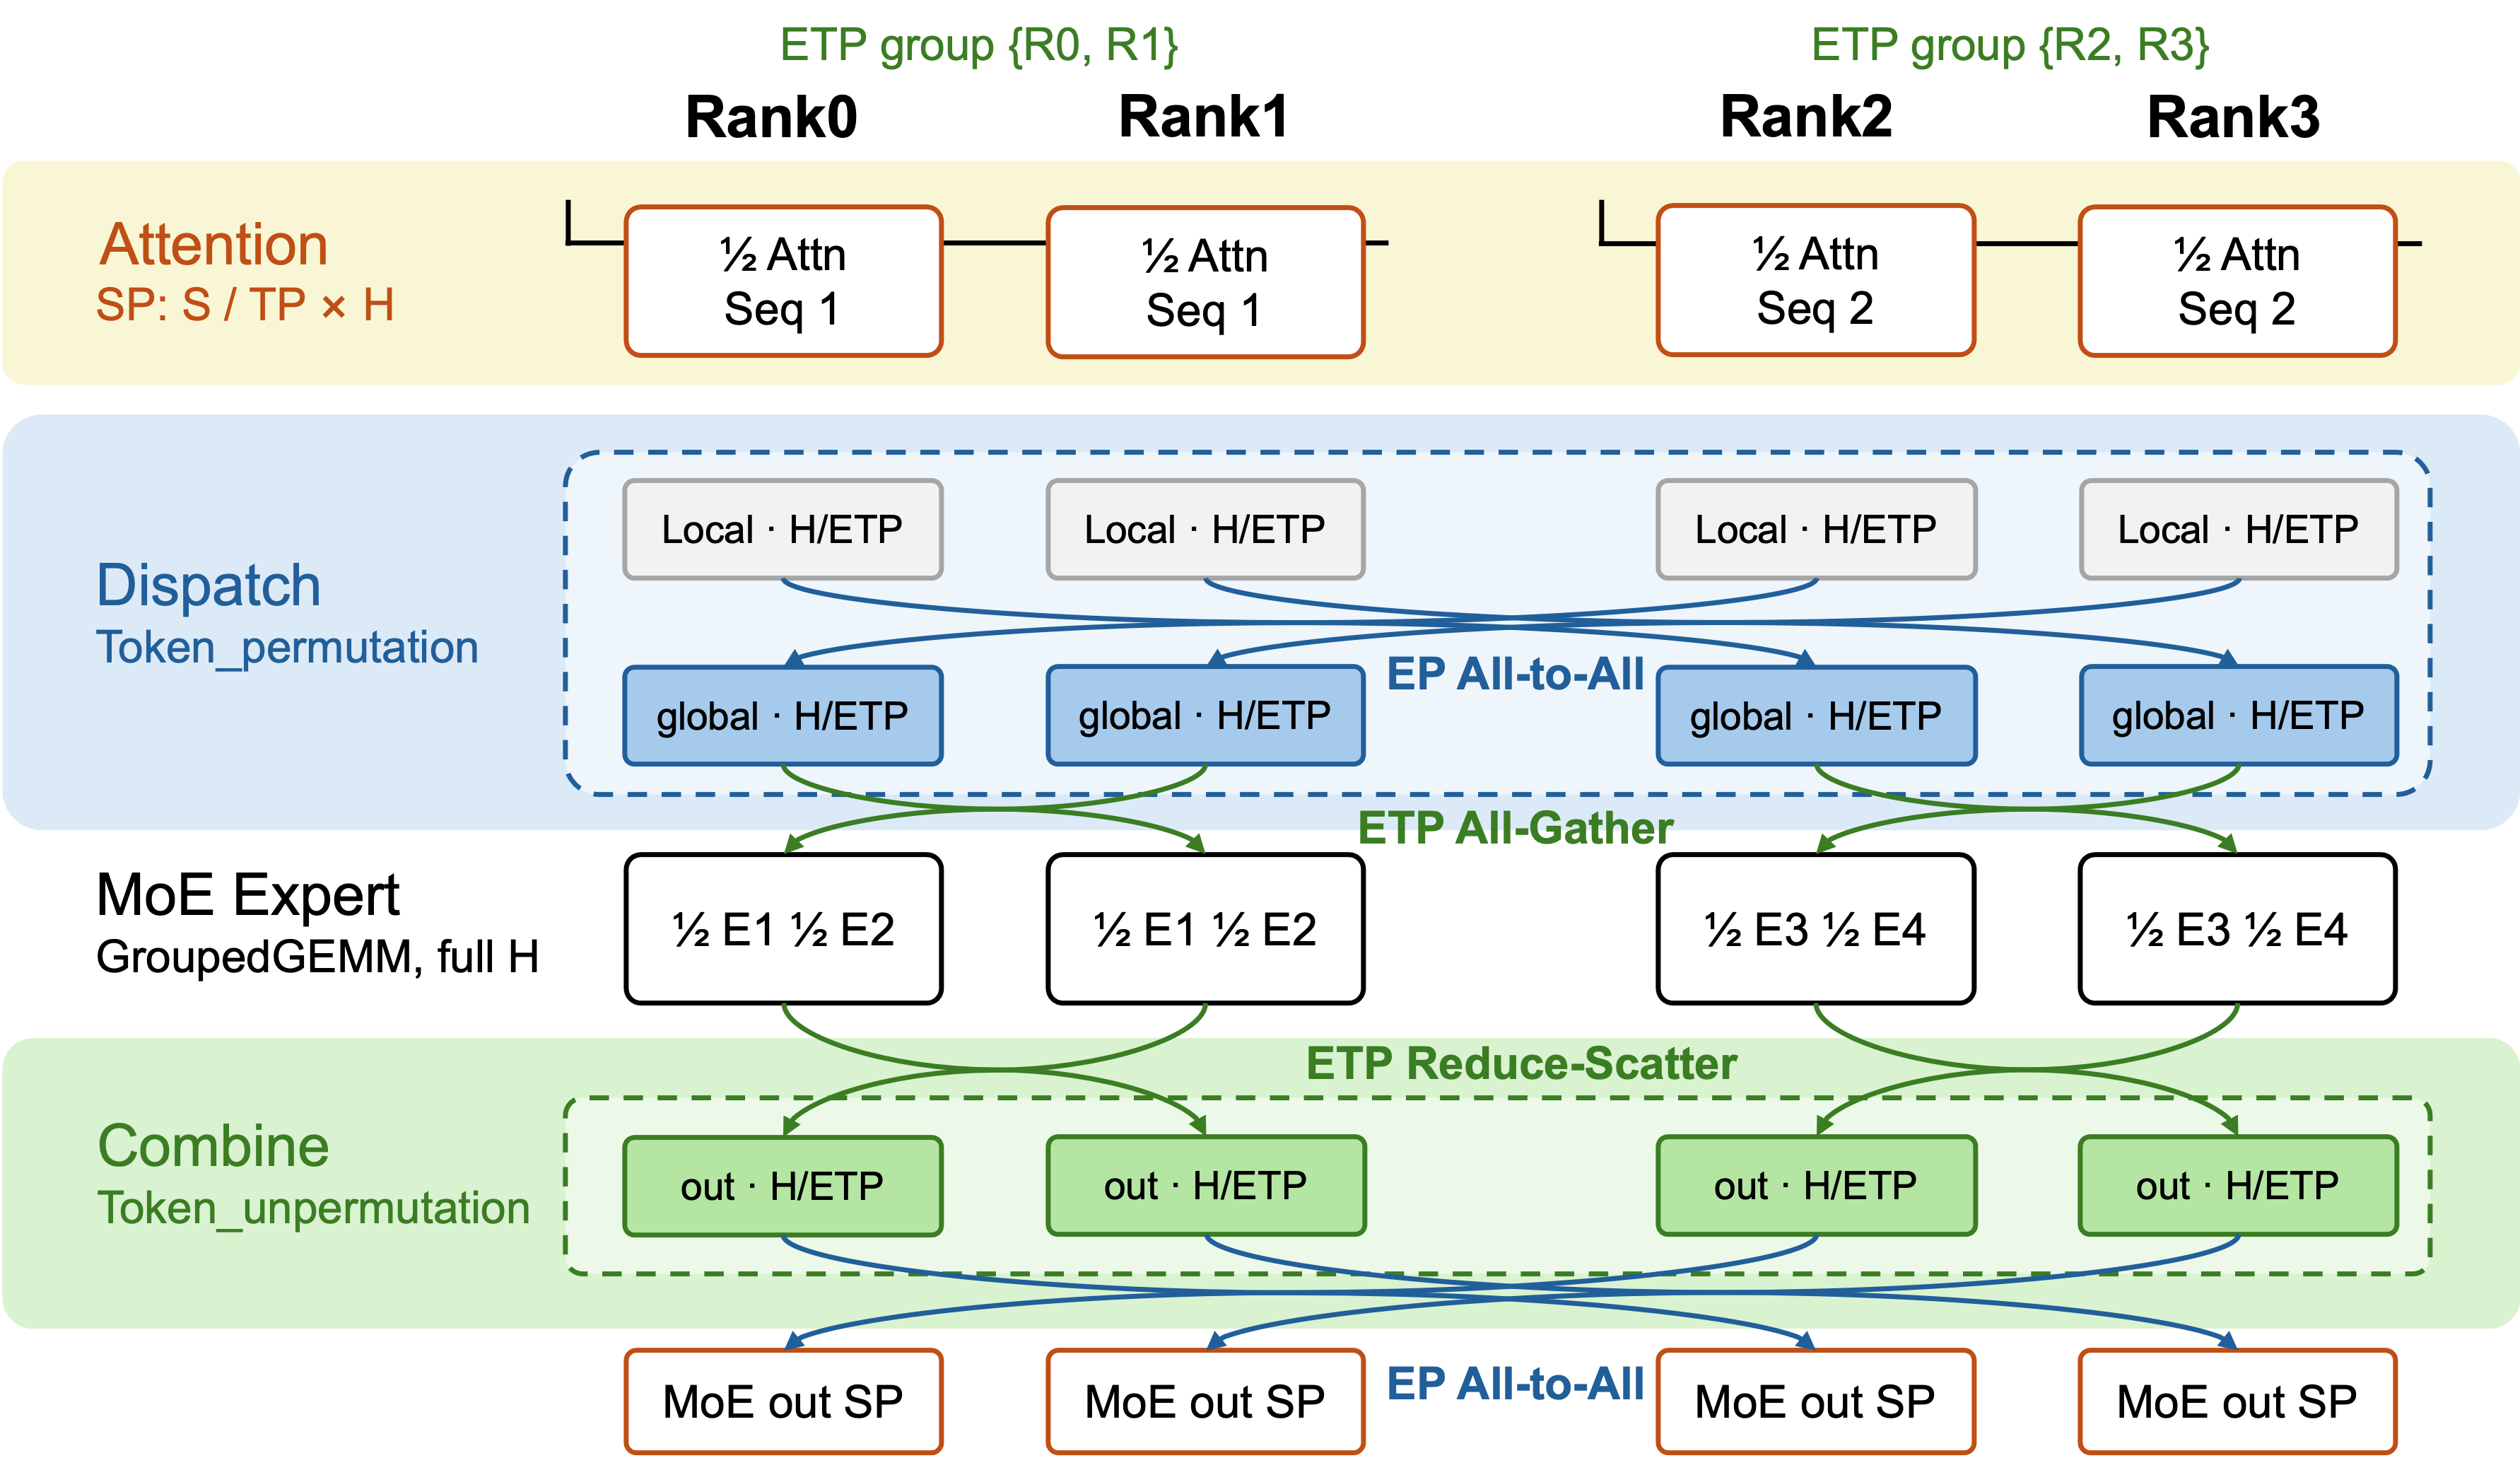
\includegraphics[width=0.9\linewidth]{figures/chapter2/ch2.2-etp.png}
\caption{Communication pattern of the ETP token dispatcher (ETP2‑EP2 example). Dispatch and combine wrap the expert grouped-GEMM with an EP all‑to‑all (token routing) and an ETP all‑gather/reduce‑scatter over the hidden dimension~\citep{gale2023megablocks}. With MoE Parallel Folding, ETP folds into EP as a single group, so one all‑to‑all performs dispatch and the separate ETP collectives are eliminated.}
  \label{fig:etp-dispatcher}
\end{figure}

% Because the extra ETP collectives add traffic to the critical path, we fold them away when the topology allows. With MoE Parallel Folding, the ETP and EP dimensions are merged into a single communication group, so one All-to-All performs dispatch and the separate ETP all-gather/reduce-scatter collectives are eliminated, reducing the number of collectives on the critical path without changing the expert-sharding layout.

\paragraph{Overlapped synchronization and computation for MoE token dispatch.}
\label{subsec:token_dispatcher}

\begin{figure}[t]
\centering
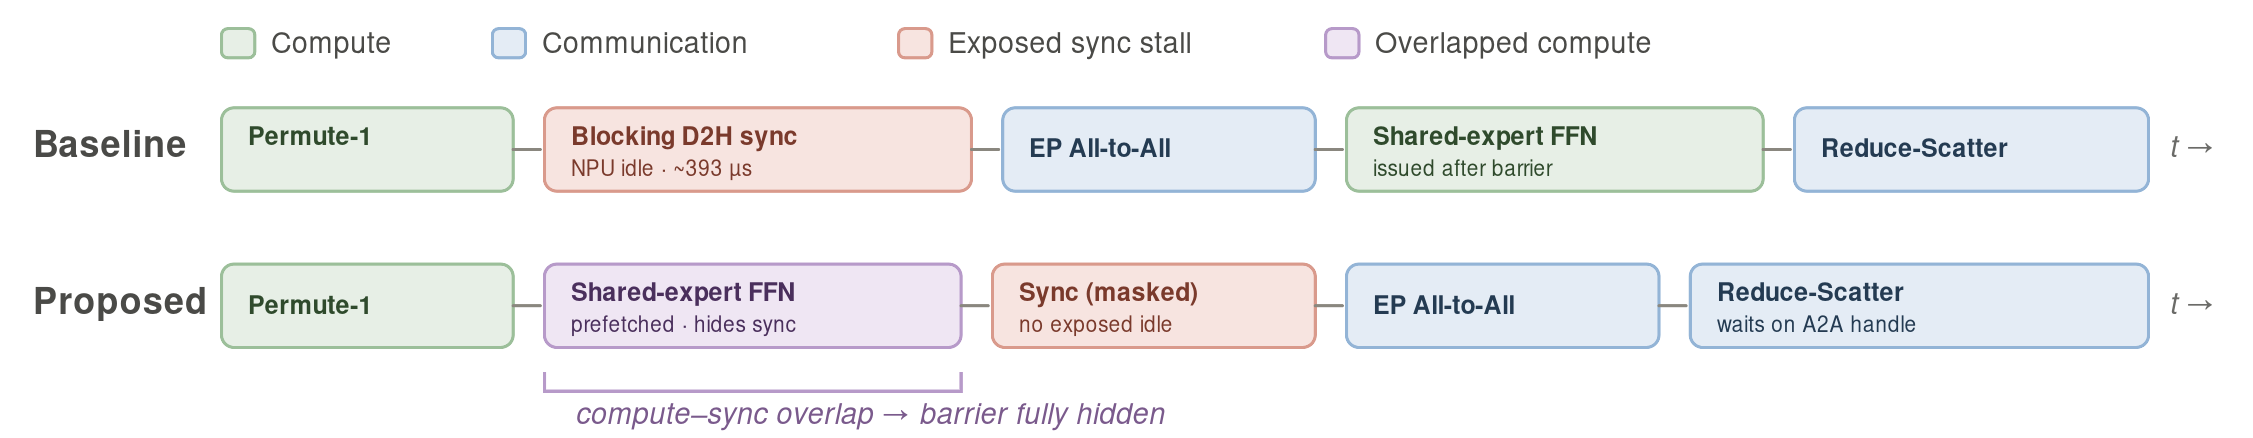
\includegraphics[width=\linewidth]{figures/chapter2/ch2.2-cover_dispatch_sync.png}
\caption{Compute--communication schedule of the MoE token dispatcher. Issuing the shared-expert forward ahead of the \texttt{before\_ep\_alltoall} synchronization fills the exposed sync stall with useful computation while communication overlap is preserved.}
  \label{fig:cover_dispatch_sync}
\end{figure}

Expert parallelism turns routing into an all-to-all (A2A) communication in distributed LLM training. 
Our dispatcher structures one MoE layer as a pipeline (permutation, an A2A dispatch, grouped-GEMM expert computation, an A2A combine, and unpermutation), and applies three Ascend-centric choices to keep the collectives off the critical path.

For the MoE module, both token dispatch and combine are implemented using asynchronous all-to-all~(A2A) collectives. Synchronization is deferred until the communicated results are consumed, allowing independent computation to execute concurrently on separate streams and thereby reducing the exposed communication latency.
Specifically for Ascend-based MoE training, we further hide the synchronization stall preceding the dispatch operation, as illustrated in Figure~\ref{fig:cover_dispatch_sync}. Because the per-expert A2A split sizes cannot be determined until token routing is completed, resolving these dynamic split sizes introduces a visible \texttt{before\_ep\_alltoall} synchronization stall on the device timeline. The shared expert, however, depends only on the MoE-layer input and is independent of the routing-derived split sizes. We therefore advance its forward computation to overlap with this synchronization interval. This scheduling strategy fills an otherwise idle period with useful Cube computation while preserving the subsequent computation-communication overlap, effectively converting the barrier-induced latency identified in Section~\ref{sec:bottleneck} into productive execution.
% , permutation and unpermutation are fused and their intermediate buffers are released eagerly, suppressing the fragmented, memory-bound tail that the same routing path would otherwise generate.

\paragraph{Double-buffered Swap Optimizer.}
\label{subsec:swap_optimizer}
At the trillion-parameter scale, optimizer states become a dominant source of device-memory consumption. Distributed AdamW~\citep{loshchilov2017decoupled} maintains an FP32 master copy of the parameters together with the first- and second-moment states, amplifying the overall HBM usage compared to the model parameters alone. 
On Ascend NPUs, enabling swap optimizer alleviates the memory pressure.

A conventional swap optimizer mitigates this pressure by offloading optimizer states~\citep{ren2021zero}, together with the FP32 master parameters when configured, to pinned host memory and reloading them only when needed for parameter updates. Although this approach reduces the HBM footprint, it introduces serialized host-to-device and device-to-host transfers around each optimizer update. These transfers extend the optimizer step and can offset the performance benefits gained from the reclaimed memory.

To reduce this overhead, we implement a double-bufferedt swap optimizer that overlaps state transfers with optimizer computation. The swapped states are partitioned into chunks of
$\texttt{swap\_numel}
= N_{\mathrm{swap}}/\texttt{swap\_optimizer\_times}$ elements, where
$N_{\mathrm{swap}}$ denotes the total number of swapped parameters. While a fused AdamW kernel updates the current chunk, the next chunk is prefetched from host memory and the previously updated chunk is asynchronously written back through dedicated swap-in and swap-out streams. This pipelined schedule removes most transfer latency from the critical path. The chunk size controls the trade-off among the temporary HBM working set, transfer granularity, and achievable overlap. As a result, the optimizer substantially reduces HBM consumption with limited runtime overhead. The reclaimed memory can support more activations and larger micro-batches, thereby reducing activation recomputation and pipeline bubbles and increasing the useful-computation share $T_{\mathrm{comp}}$.

\subsection{Kernel Optimization for Accelerated LLM Training}
\label{sec:kernel_opt}

\subsubsection{Bottleneck Kernel Analysis}
\label{sec:kernel_bottleneck}

% Training DeepSeek-V4-Pro on Ascend CloudMatrix384 involves a heterogeneous mix of compute-intensive operators whose execution efficiency critically determines overall Model FLOPs Utilization (MFU).
% To precisely characterize the dominant compute bottlenecks, we conduct comprehensive application-level profiling using across all NPU ranks during representative training steps.


% The primary performance indicator is \textbf{Task Duration}, which measures end-to-end wall-clock time per operator invocation and serves as the definitive optimization target. Beyond this primary signal, A suite of auxiliary metrics are exposed that decompose the execution into compute and data-movement components.
% Following the step-level decomposition in Section~\ref{sec:bottleneck}, we focus on the optimization of NPU kernels for training. 
% A more detailed perspective of kernel computation reviews the AI Core computing bottleneck while demonstrating its launch-level boundaries, which further yields two directions of optimization. 
% A small set of architecture-defined kernels, such as sparse attention, dense projections, and grouped expert computation, concentrate device time in individual invocations. 
% In parallel, several model-specific stages are still expressed through torch-based Python-level combination and perform the runtime as chains of casts, views, tensor moves, and reductions, which leads to repetitive kernel launching. 

% We construct the profile around the unit at which an optimization can act. Task Duration identifies kernels that occupy the device timeline and are candidates for kernel-internal tuning. Launch counts and submodule labels recover how high-level model stages are decomposed by the runtime. For vector-core kernels, the AIV pipeline counters---vector-compute, scalar, MTE2 load, and MTE3 store ratios---separate arithmetic from data movement. Read together, these measurements distinguish a standalone heavy kernel from a launch-fragmented operator chain, and both from a memory-traffic pattern created by the frontend expression.

% The resulting profile contains $52{,}376$ compute-kernel launches and $10.68$\,s of aggregate device-side compute duration after excluding communication and AI-CPU runtime. Within this device-compute view, the profile resolves into four patterns that recur throughout the analysis below: a small heavy head of architecture-intrinsic kernels whose cost lies inside the kernel body; a launch-fragmented tail of eager torch chains, where the cost is the sheer number of kernel boundaries; a memory-bound vector tail, where each kernel spends most of its time moving data rather than computing; and a set of generic Triton kernels whose arithmetic is sound but whose lowering leaves on-chip residency and pipeline scheduling on the table. The first is a kernel-internal problem; the other three are addressed by re-expression into Unified-Buffer-resident AscendC kernels. Table~\ref{tab:kernel_bottleneck} reports representative top operators and their vector-pipeline decomposition, and we take the head and the tail in turn.
Following the training step-level decomposition in Section~\ref{sec:bottleneck}, we further investigate the device-compute bottlenecks at the kernel level. The profiling results reveal two distinct sources of inefficiency. \circled{1}~The  architecture-intrinsic kernels, including sparse attention, dense matrix multiplications, and grouped expert GEMMs, account for substantial device time within individual invocations. \circled{2}~Model-specific stages remain implemented as PyTorch-level compositions and are lowered by the \texttt{eager mode} into long sequences of casts, views, tensor-movement, and reductions, resulting in excessive kernel launches and fragmented execution. These observations motivate two complementary optimization directions: kernel-internal tuning for dominant compute-intensive kernels, and fusion or re-expression for launch-fragmented operator chains.

We organize the profiling results at the granularity at which optimization decisions can be made. Task Duration identifies individual kernels that dominate the device timeline and are therefore candidates for kernel-internal optimization. Kernel launch counts and submodule annotations reveal how high-level model stages are decomposed into low-level runtime operations. For AIV-dominated kernels, the utilization ratios of the vector-compute, scalar, MTE2 load, and MTE3 store pipelines further indicate whether execution is constrained by arithmetic, scalar control, or data movement. Taken together, these measurements distinguish compute-intensive standalone kernels from launch-fragmented operator chains and from memory-traffic bottlenecks introduced by the frontend implementation.

On the profiled NPUs, the trace contains $206{,}503$ compute-kernel launches and $39.84$\,s of aggregate device-side compute duration after excluding communication and AI-CPU execution. The resulting kernel profile exhibits four recurring patterns. The first is a small heavy head of architecture-intrinsic kernels whose latency is dominated by computation within the kernel body. The second is a launch-fragmented tail produced by PyTorch \texttt{eager computation}, where overhead accumulates across a large number of short-lived kernels. The third is a memory-bound vector tail, in which execution time is dominated by data movement rather than arithmetic. The fourth consists of generic Triton-generated kernels whose functional computation is correct, but whose lowering does not fully exploit on-chip data residency or pipeline scheduling. The first category primarily requires kernel-internal optimization, whereas the remaining categories motivate operator fusion or re-expression as AscendC kernels that retain intermediate tensors in Unified Buffer whenever possible. Table~\ref{tab:kernel_bottleneck} summarizes representative operators and their vector-pipeline characteristics. We first examine the dominant kernels and then turn to the fragmented and memory-bound long tail.





% TODO: Fill with actual profiling data once available
% \begin{table}[h]
	% \centering
	% \caption{Top bottleneck operators in DeepSeek-V4-Pro training on Ascend 910C.}
	% \label{tab:kernel_bottleneck}
	% \resizebox{\textwidth}{!}{%
		% \begin{tabular}{clccccc}
			% \toprule
			% Rank & Operator & \makecell{Task Duration\\Share ()} & Vec Ratio & \makecell{AIV MTE2\\Ratio} & \makecell{AIV MTE3\\Ratio} & \makecell{AIV Scalar\\Ratio} \\
			% \midrule
			% 1 & \textit{[e.g., Multi-Head Latent Attention Fwd]} & --- & --- & --- & --- & --- \\
			% 2 & \textit{[e.g., Expert GEMM / MoE Dispatch]} & --- & --- & --- & --- & --- \\
			% 3 & \textit{[e.g., Flash MLA Backward]} & --- & --- & --- & --- & --- \\
			% 4 & \textit{[e.g., RMSNorm Fused]} & --- & --- & --- & --- & --- \\
			% 5 & \textit{[e.g., Expert Router / Token Scatter]} & --- & --- & --- & --- & --- \\
			% \bottomrule
			% \end{tabular}}
	% \end{table}




% \begin{table}[htp]
	% \centering
	% \caption{Representative top operators in DeepSeek-V4-Pro training on Ascend 910C, ranked by Task Duration share as reported by on-device profiling tooling. Each operator's share is its summed core-busy time (the per-kernel AI-Core or vector-core execution time) normalized against the summed core-busy time of all compute kernels, after excluding communication and AI-CPU entries; this is the base reported under the tool's ``Task Duration'' column. Invocation count and average per-call duration are also reported to expose the fragmented, long-tailed nature of the memory-bound operators. Matrix-multiplication (cube) operators are reported with AIC counters (MAC, MTE2, Fixpipe store, and cube utilization), while vector operators are reported with AIV counters (vector compute, MTE2, MTE3, and scalar utilization); the store column is therefore MTE3 for vector rows and Fixpipe for cube rows, and entries inapplicable to a pipeline are shown as ``\,--\,''. Even within the cube kernels the pressure differs: \texttt{GroupedMatmul} is genuinely MAC-dominated ($87.0\%$ MAC at $95.4\%$ utilization), whereas \texttt{MatMulV3} is operand-load-bound, its MTE2 load share ($96.3\%$) far exceeding its MAC share ($52.6\%$). The vector rows sit at the opposite end, with compute shares well below their MTE shares. The final row aggregates the remaining $93$ operator types---a long tail of small, memory-bound vector and copy kernels that individually rank low but collectively account for $38.4\%$ of the Task Duration share across $32{,}449$ launches, and which the operator-chain fusion of Section~\ref{sec:kernel_fusion} targets.}
	% \label{tab:kernel_bottleneck}
	% \resizebox{\textwidth}{!}{%
		% \begin{tabular}{clcrrcccc}
			% 	\toprule
			% 	Rank & Operator & \makecell{Task Dur.\\Share} & Calls & \makecell{Avg\\($\mu$s)} & \makecell{Compute\\(MAC/Vec)} & \makecell{MTE2\\Load} & \makecell{Store\\(MTE3/Fix)} & \makecell{Cube/Scalar\\Util.} \\
			% 	\midrule
			% 	1 & \texttt{SparseAttnSharedkvGrad} (sparse-attn bwd) & $16.33\%$ & $56$    & $28{,}708$ & $9.2\%$  & $21.4\%$ & $34.5\%$ & $92.1\%$ \\
			% 	2 & \texttt{MatMulV3}                                 & $11.88\%$ & $1{,}400$ & $1{,}056$  & $52.6\%$ & $96.3\%$ & $21.9\%$ & $85.4\%$ \\
			% 	3 & \texttt{GroupedMatmul} (MoE experts)              & $8.82\%$  & $336$   & $2{,}601$  & $87.0\%$ & $96.2\%$ & $11.4\%$ & $95.4\%$ \\
			% 	4 & \texttt{Cast}                                     & $5.69\%$  & $10{,}039$ & $59$    & $5.7\%$  & $90.2\%$ & $60.5\%$ & $1.7\%$ \\
			% 	5 & \texttt{SparseLightningIndexerGradKLLoss}         & $5.48\%$  & $24$    & $22{,}471$ & $10.4\%$ & $19.5\%$ & $13.8\%$ & $96.0\%$ \\
			% 	6 & \texttt{Add}                                      & $5.02\%$  & $4{,}171$ & $133$    & $14.0\%$ & $93.3\%$ & $22.9\%$ & $2.3\%$ \\
			% 	7 & \texttt{Mul}                                      & $3.20\%$  & $3{,}677$ & $89$     & $39.1\%$ & $53.7\%$ & $20.1\%$ & $10.7\%$ \\
			% 	8 & \texttt{SparseAttnSharedkv} (sparse-attn fwd)     & $2.62\%$  & $112$   & $2{,}505$  & $43.1\%$ & $51.4\%$ & $30.3\%$ & $87.7\%$ \\
			% 	9 & \texttt{RmsNormWithoutWeight} (Triton)            & $2.60\%$  & $112$   & $2{,}300$  & $29.5\%$ & $49.8\%$ & $29.8\%$ & $33.5\%$ \\
			% 	\midrule
			% 	\multicolumn{2}{l}{Long tail ($93$ remaining operator types)} & $38.36\%$ & $32{,}449$ & $\approx 128$ & \multicolumn{4}{l}{predominantly small, memory-bound vector \& copy kernels} \\
			% 	\bottomrule
			% 	\end{tabular}}
	% \end{table}

We begin with the dominant kernels, a small set of architecture-specific operations that account for a substantial fraction of device-compute time. 
In particular,  \texttt{SparseAttnSharedkvGrad} is the largest individual contributor, accounting for $16.86\%$ of the total kernel computation time due to the expensive gradient computation with respect to the DeepSeek sparse attention. 
Unlike ordinary operators~(e.g., Matrix Multiplication) which are thoroughly optimized, architecture-specific kernels exhibits high code-level complexity in hierarchical memory layout and computation pipelines.
This work addresses the challenge of kernel complexity via the proposed \textbf{AuraKernel} agent, as elaborated in Section~\ref{sec:kernel_agent}.

% The heavy head is formed by operators that come directly from the DeepSeek-V4-Pro architecture. The shared-key-value sparse-attention backward, \texttt{SparseAttnSharedkvGrad}, is the single largest core-time contributor at $16.33\%$ of the Task Duration share reported by the profiling tool, followed by dense matrix multiplication (\texttt{MatMulV3}, $11.88\%$) and Mixture-of-Experts expert multiplication (\texttt{GroupedMatmul}, $8.82\%$). The sparse-attention forward pass (\texttt{SparseAttnSharedkv}, $2.62\%$) and its Lightning-indexer gradient with KL loss (\texttt{SparseLightningIndexerGradKLLoss}, $5.48\%$) add further architecture-intrinsic cost. These kernels directly implement the model's sparse-attention and MoE computation. Their optimization space is inside the kernel body: tiling, pipeline overlap, memory layout, and hardware-specific scheduling. This part of the profile motivates the automated, profiling-in-the-loop kernel tuning performed by AuraKernel in Section~\ref{sec:kernel_agent}.


\begin{figure}[h]
	\centering
	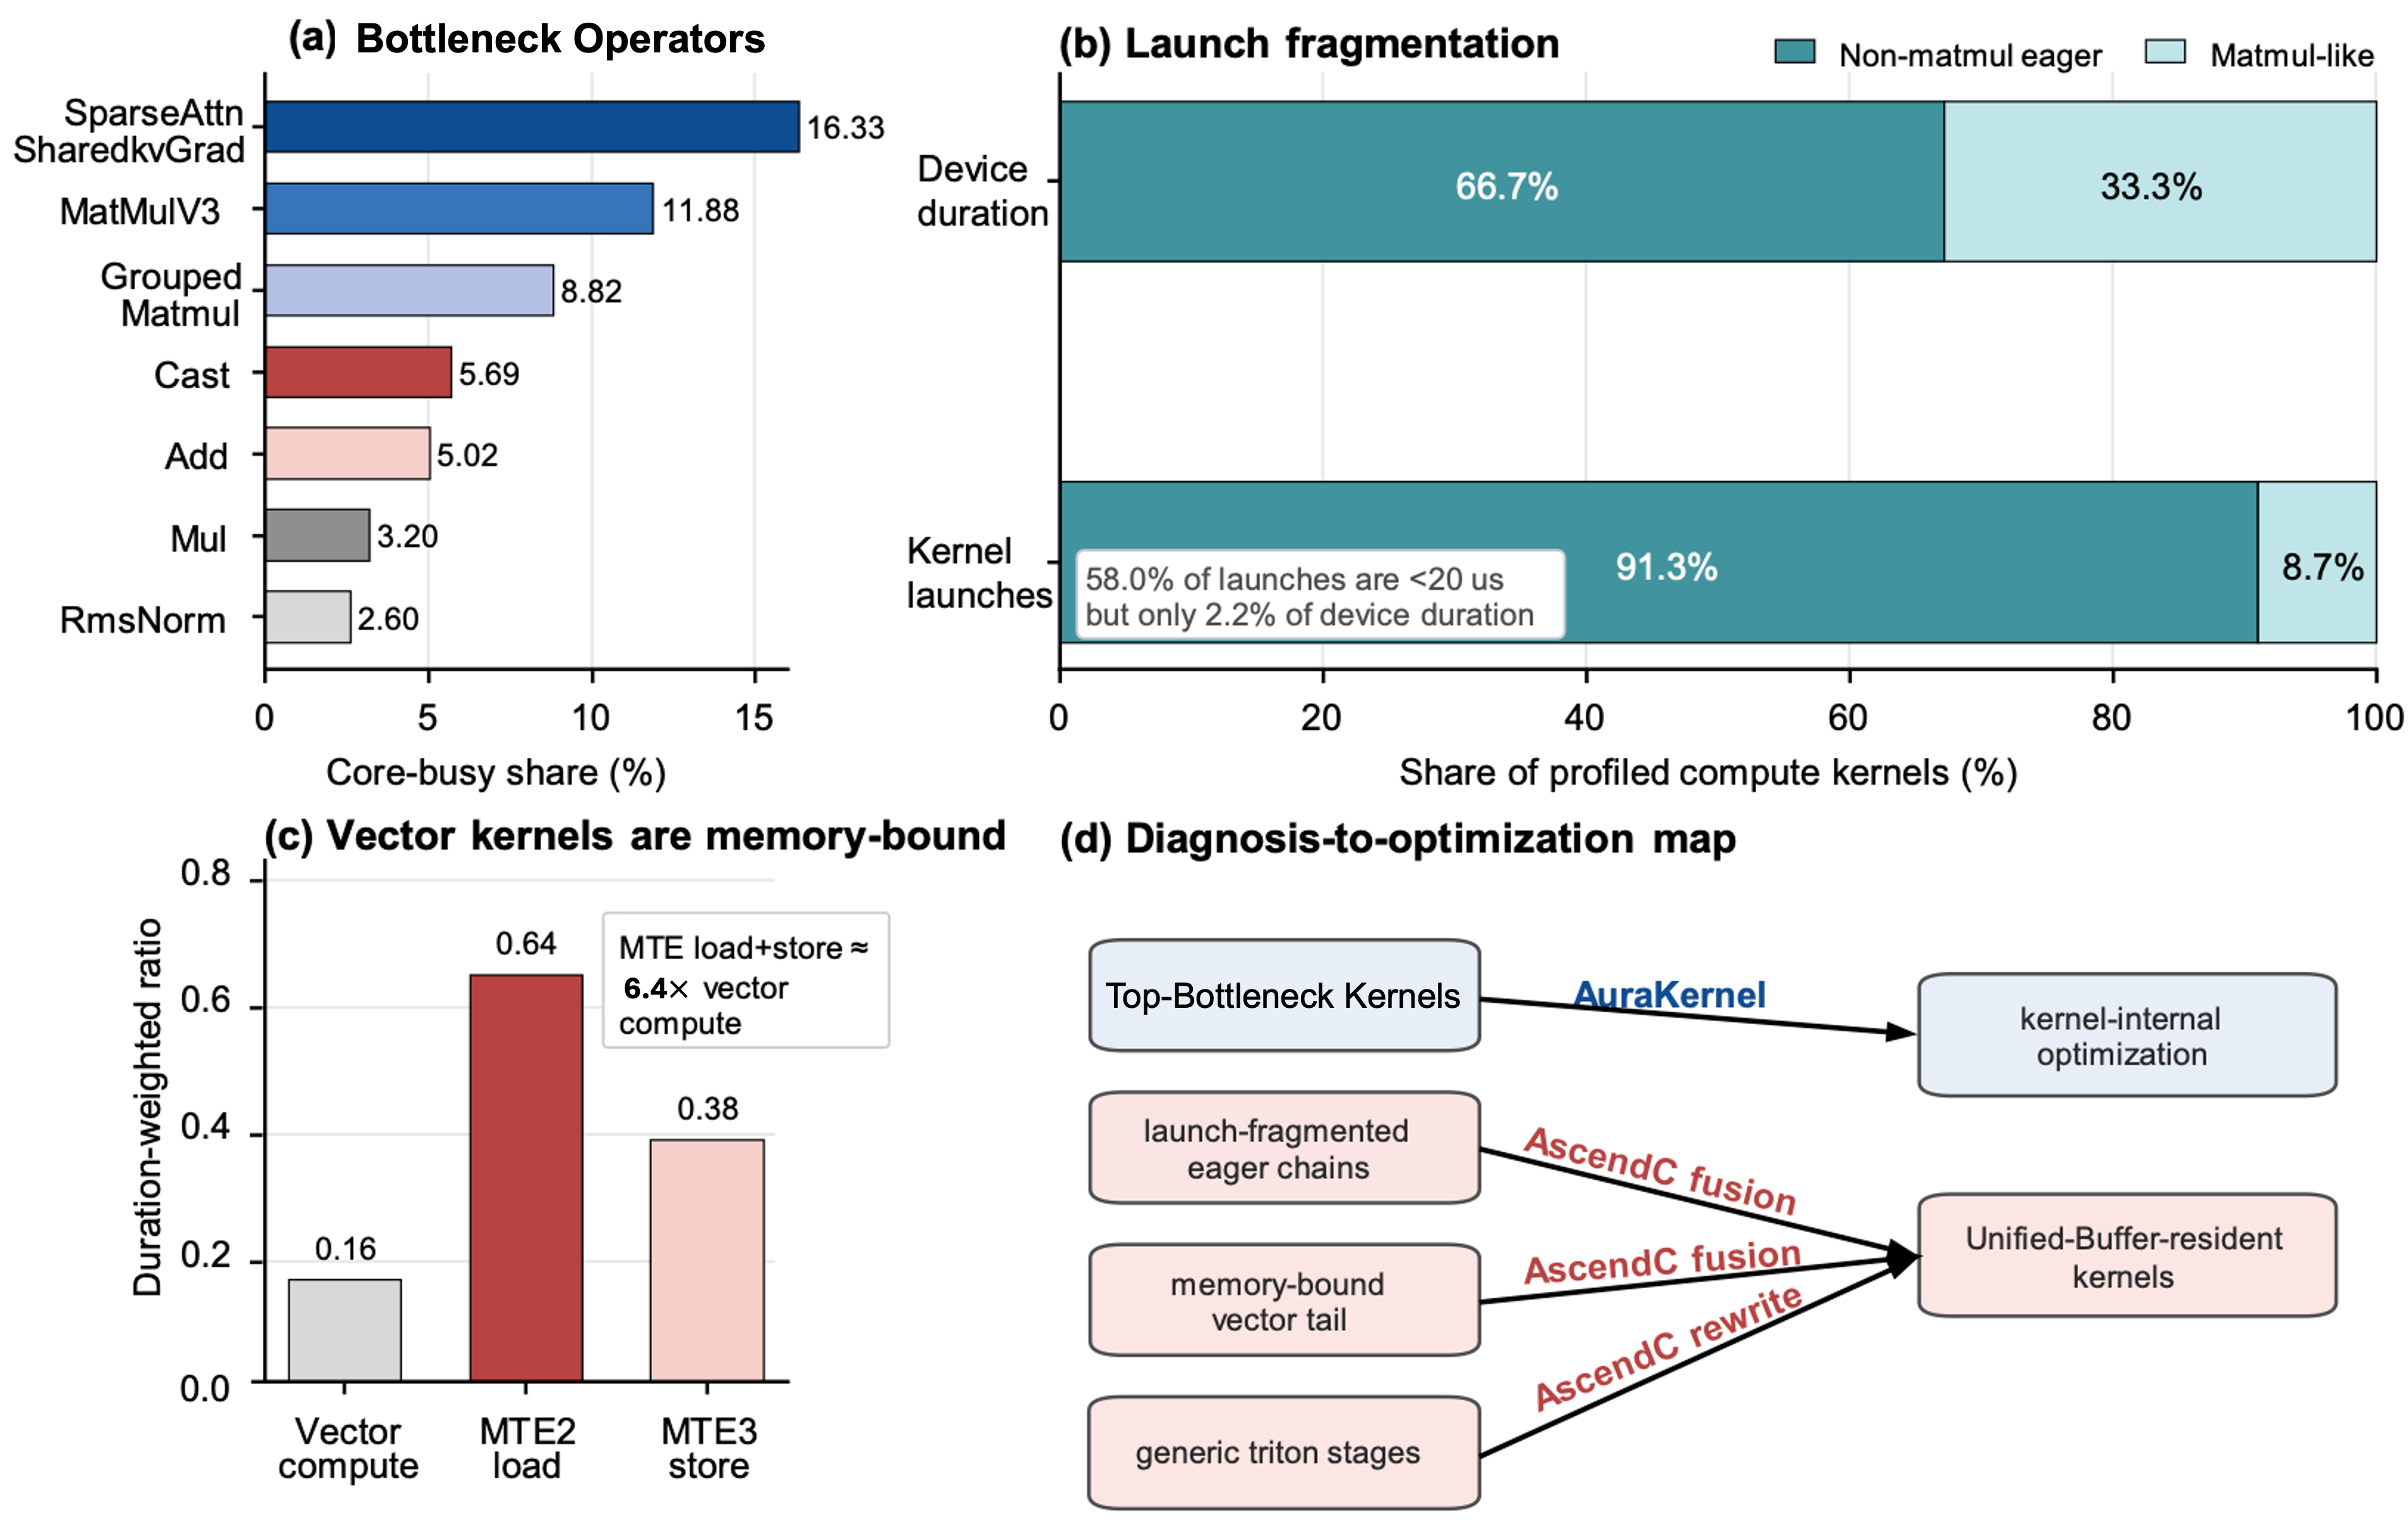
\includegraphics[width=\textwidth]{figures/chapter2/ch2.2.1-bottleneck_anatomy_v3.png}
	\caption{Bottleneck anatomy of one representative DeepSeek-V4-Pro training step on Ascend 910C ($206{,}503$ compute kernels, $39.84$\,s device-side duration). Panel~(a): the heavy head of architecture-intrinsic operators by core-busy share (the tool's ``Task Duration'' column)---sparse-attention backward, dense matrix multiplication, and grouped MoE multiplication. Panel~(b): the complementary launch-fragmentation view, contrasting the launch share of non-matmul eager operators with their much smaller share of device duration, and isolating the dense sub-$20\,\mu$s tail. Panel~(c): duration-weighted vector-pipeline ratios---vector compute well below the MTE2 load and MTE3 store ratios, whose combined memory movement is about $7.4\times$ the vector-compute share. Panel~(d): the resulting division of work---architecture-intrinsic heavy-head kernels routed to kernel-internal optimization by AuraKernel, and the launch-fragmented, memory-bound, and generic-Triton tails routed to re-expression as UB-resident AscendC kernels.}
	\label{fig:bottleneck_anatomy}
\end{figure}

The same trace also exposes a second execution regime. Rotary position embedding, weight-free RMS normalization, limited SwiGLU, and the mHC projection path are implemented as torch-level compositions, and autograd expands them into long sequences of generic operators. In the profiled step, non-matmul eager operators account for $91.3\%$ of launches but only $66.7\%$ of the Task Duration, against $33.3\%$ for the far fewer matmul-like operators (Figure~\ref{fig:bottleneck_anatomy}b). A dense small-kernel tail gives the regime its shape: $58.0\%$ of launches finish in under $20\,\mu$s yet together contribute only $2.2\%$ of Task Duration. The performance cost is therefore caused by repetition and by the boundaries between kernels: tensor materialization, dispatch, scheduling, and memory traffic are paid at every link in the chain.

The vector-pipeline counters show that the long tail is primarily constrained by data movement rather than arithmetic. Vector-core kernels account for $36.5\%$ of the total Task Duration, but their vector-compute utilization is only about $15\%$, substantially lower than the corresponding MTE load and store ratios of approximately $68\%$ and $40\%$, respectively (Figure~\ref{fig:bottleneck_anatomy}c). The imbalance indicates that most vector-kernel execution time is consumed by loading, storing, and rearranging data instead of actual computation.

The distribution of operators~(frequency and latency) further confirms that the long tail is dominated by fragmented data-movement operations. \texttt{Cast} is invoked $40{,}063$ times and contributes $6.02\%$ of the total Task Duration, while operators such as \texttt{ViewCopy}, \texttt{TensorMove}, \texttt{ZerosLike}, and \texttt{Slice} introduce additional overhead through frequent tensor materialization and buffer movement. These operations commonly arise when high-level backward computations, such as rotary embedding and limited SwiGLU, are decomposed into multiple small kernels under eager execution.

The bottleneck analysis motivates two separate kernel-optimization paths. Architecture-intrinsic kernels are optimized within the operator through improved tiling, data layout, scheduling, and pipeline overlap, which can be performed via agentic pipeline with long-context understanding~(Section~\ref{sec:kernel_agent}). On the other hand, the fragmented long tail is addressed by fusing and rewriting each target stage as a hardware-aware AscendC kernel. For eager autograd chains, this requires recovering the high-level computation and eliminating unnecessary data movement and type conversion introduced by framework execution. For existing Triton kernels, the computation is reimplemented in AscendC with explicit control over Unified Buffer~(UB) residency, tiling, and MTE scheduling. Both approaches reduce global-memory traffic by retaining intermediate results on-chip and consolidating the computation into fewer kernel passes. Section~\ref{sec:kernel_fusion} describes this fusion-and-rewrite path in detail.


\subsubsection{AuraKernel: Performance Optimization Agent for Complex Ascend Kernels}
\label{sec:kernel_agent}

\begin{figure}[t]
  \centering
  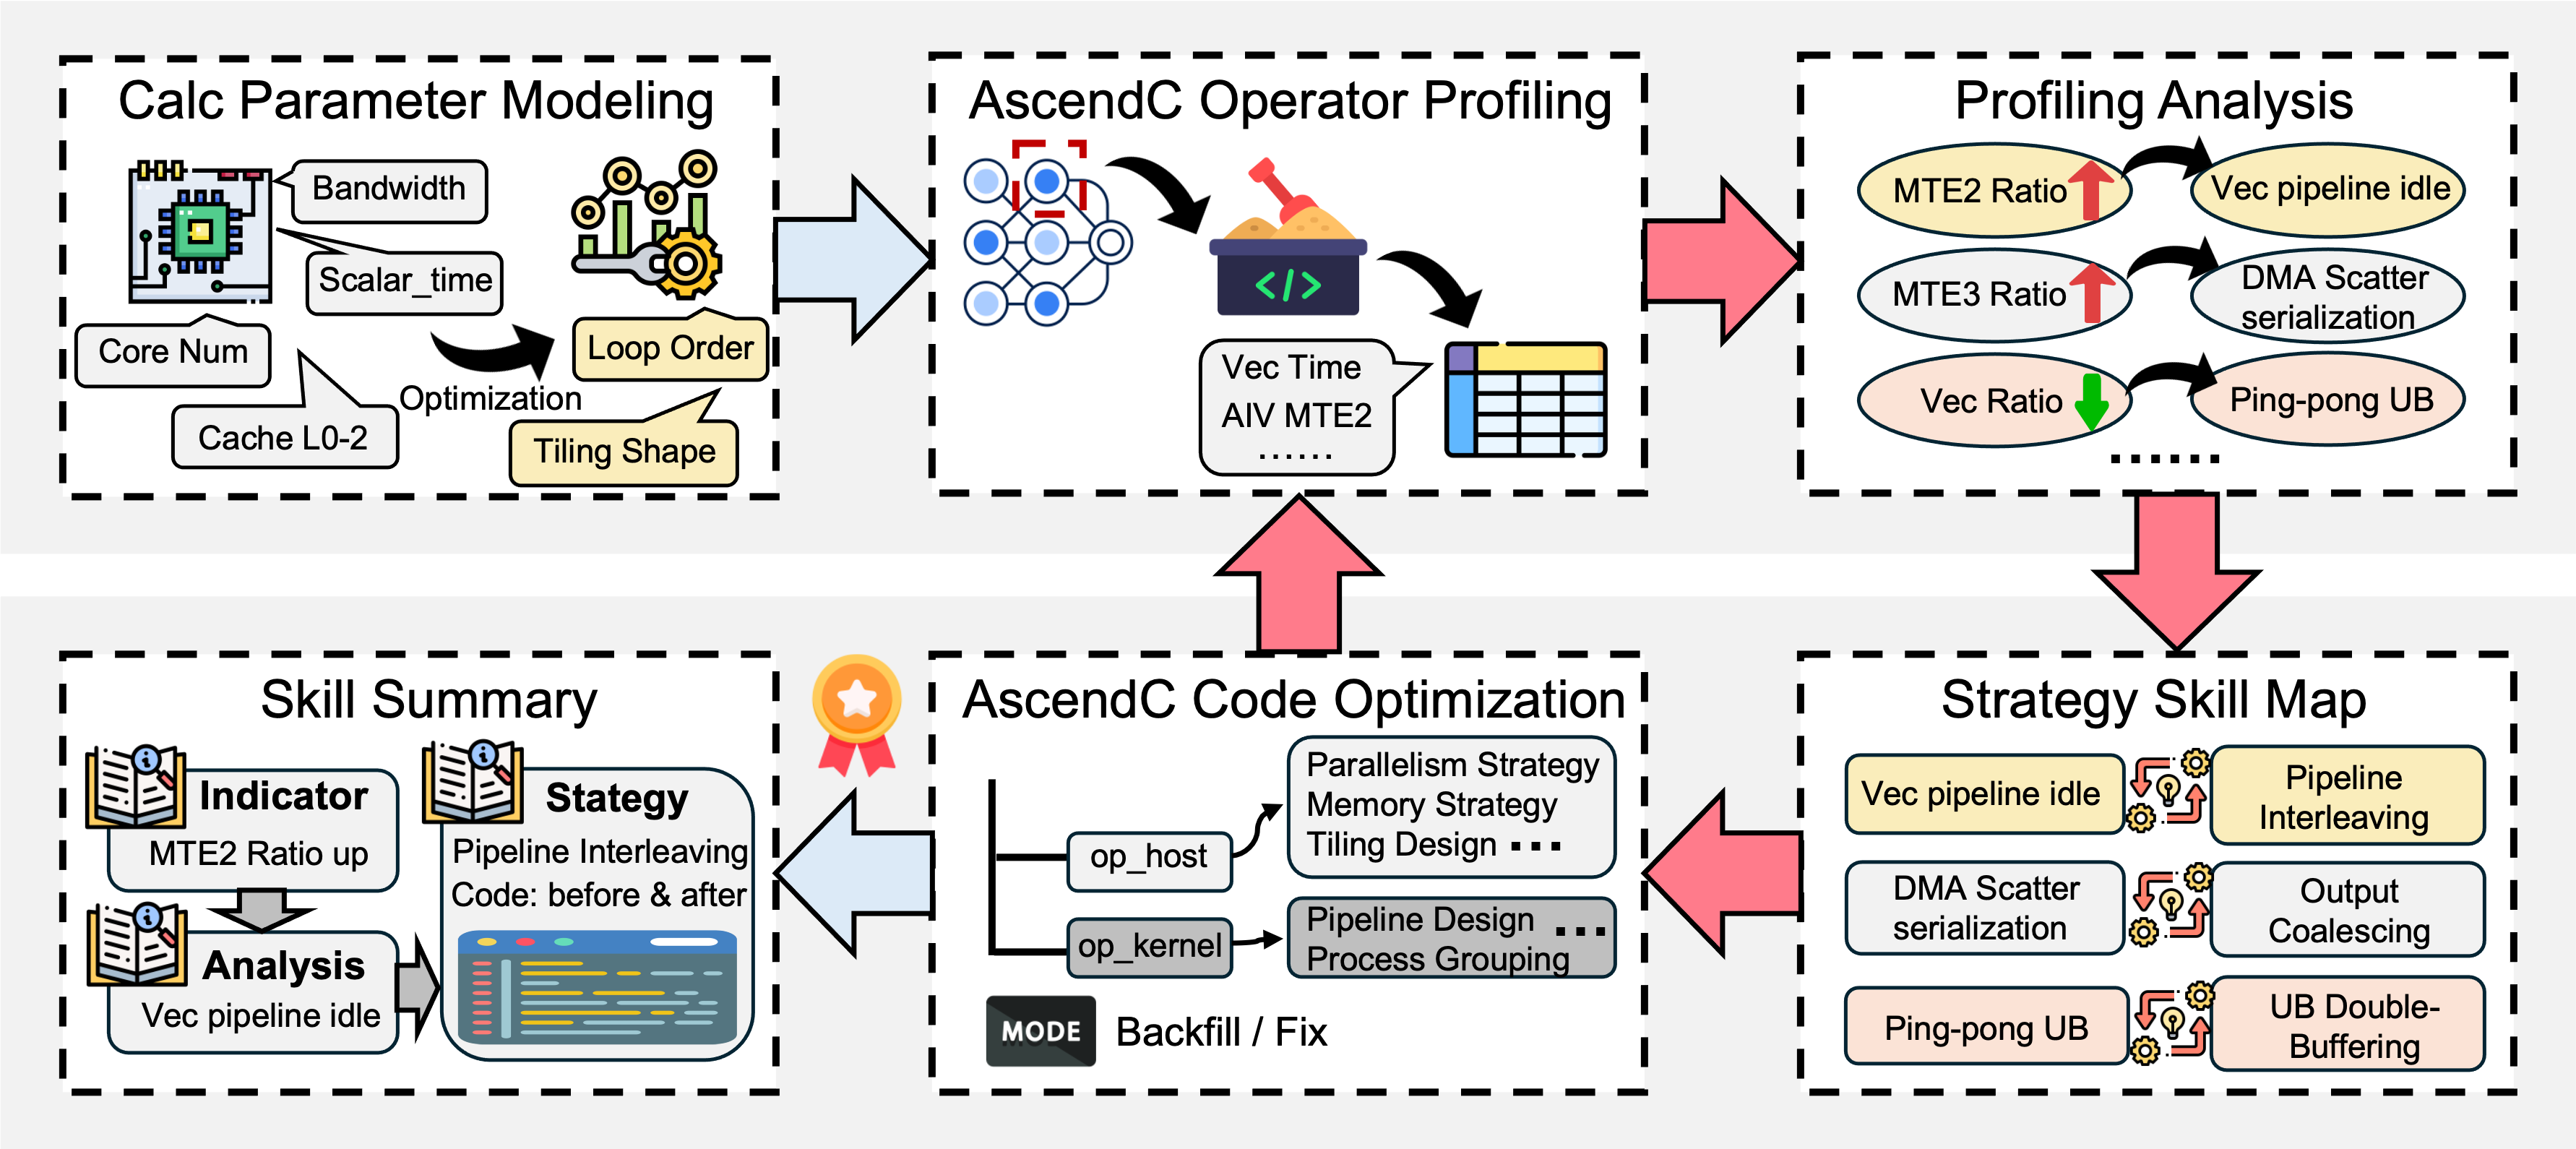
\includegraphics[width=1.0\textwidth]{figures/aurakernel.png}
  \caption{The architecture of AuraKernel. Starting from a functionally correct baseline kernel, AuraKernel generates an optimized operator in three stages. (1)~\textbf{OR-based tiling optimization} diagnoses the operator's dominant regime and instantiates a hardware-aware parameter space, yielding an initial configuration and a set of promising optimization directions. (2)~\textbf{Hardware-grounded iterative optimization} runs a closed modify--verify--profile loop: a harness compiles each candidate, gates it on correctness with the returnd profiling, while K-Search uses this feedback to explore a branchable, rollbackable tree of optimization directions and commits a checkpoint on every verified improvement. (3)~\textbf{Skill distillation} converts each verified gain into a reusable skill that is retrieved to guide hypothesis generation in later episodes.}
  \label{fig:aurakernel}
\end{figure}

Achieving high kernel efficiency on Ascend 910C is fundamentally different from optimizing CUDA kernels. 
Benefiting from the well-established open-source community with diverse data sources, CUDA-based kernel writing has been widely studied and used to train in recent LLM models~\citep{dao2022flashattention,dao2023flashattention2,shah2024flashattention3,tillet2019triton,hsu2024liger,ye2025flashinfer,wei2025astra,dong2025stark}. 
However, agent-based kernel optimization for non-CUDA hardware remains challenging due to uncommon hardware architecture and programming languages. 
With fine-grained memory control and pipeline, optimizing Ascend operators via agent system faces two critical challenges: 
\begin{itemize}
\item \textbf{Operator optimization with disaggregated host-kernel design:}
Unlike CUDA kernels, a complete AscendC operator package consists of \textbf{both} host-side scheduling logic and device-side kernel implementation, enabling flexible control over execution parameters such as tiling, memory movement, and launch configuration. Optimizing AscendC operators therefore requires the agent to reason beyond isolated kernel code and understand the explicit contract between the host and device sides.

\item \textbf{Long-context understanding with hierarchical agent memory:} 
Complex AscendC operators, such as sparse-attention kernels, often involve long-range code dependencies, multi-stage data movement, stream-level coordination, and pipeline scheduling. During iterative hardware-agent interaction, the agent must preserve and retrieve relevant design decisions, profiling observations, and correctness constraints across long optimization trajectories. Effective hierarchical memory is therefore essential for maintaining optimization consistency and avoiding repeated or conflicting modifications.

\item \textbf{Heuristic optimization leads to suboptimal efficiency:} 
Existing AscendC operator optimization still heavily relies on expert-crafted heuristics for tiling, buffering, and pipeline scheduling. However, these heuristics are often hardware-, shape-, and operator-specific, making them difficult to generalize across diverse workloads. 
As a result, purely heuristic optimization can easily converge to locally efficient but globally suboptimal configurations, motivating a more systematic optimization framework that combines Kernel agent with mathematical modeling~(for optimal initialization) followed by iterative hardware feedback.
\end{itemize}
% GPU optimization now benefits from a well-established ecosystem and open-sourced communities, including IO-aware algorithmic kernels, Triton-style DSLs, fused LLM-training libraries, and emerging LLM-based CUDA optimization agents

% These methods work partly because modern LLMs have absorbed abundant CUDA code, cuBLAS/CUTLASS idioms, and warp-level scheduling patterns from public corpora. AscendC, in contrast, exposes a more hardware-explicit programming model through CANN: performance depends on coordinating data movement across the Ascend memory hierarchy, selecting valid tiling parameters, and matching the host-side tiling program with the kernel-side pipeline schedule. A locally good tiling choice can still induce DMA stalls, poor buffer reuse, or pipeline imbalance once combined with the actual kernel implementation.

% This makes Ascend 910C kernel optimization both high-impact and knowledge-scarce. 
Recent AscendC kernel agents focus on domain-specific training, DSL-guided generation, and profiling-in-the-loop search~\citep{ascendkernelgen2026,ascendcraft2026,wu2025ascendoptimizer}. However, production LLM training introduces a stricter setting: the target kernels must be optimized under real application shapes, memory pressure, layout constraints, and profiling signals from the end-to-end training workload rather than isolated microbenchmarks. 

In this work, we propose \textbf{AuraKernel}, a performance optimization agent for AscendC kernels.  Figure~\ref{fig:aurakernel} presents the system-level design of AuraKernel. 
The agent first builds a hardware-aware parameter model to constrain the optimization space; it then enters a profiling-driven loop that diagnoses bottleneck indicators, maps them to concrete optimization strategies, and applies code rewrites; finally, successful indicator--strategy--code patterns are distilled into reusable skills. 
%We organize the following discussion according to these stages.

\paragraph{Optimized Tiling Strategy via Operations Research.}
Given a pre-crafted AscendC kernel, AuraKernel initializes the optimization process with a solver-guided tiling strategy tailored to the target computation shape. Instead of relying solely on heuristic search, AuraKernel formulates operator tuning as a constrained performance-modeling problem. The optimizer determines how the workload is partitioned across AI Cores, how tiles are staged through GM, L2, L1, L0, and UB, how DMA transfers are overlapped with CUBE or vector execution, and how intermediate results are written back.

Given an operator shape, AuraKernel first identifies its dominant execution regime, such as compute-bound, memory-bound, scalar/control-bound, or communication-bound. It then instantiates a family-specific parameter space. For GEMM-like compute kernels, the parameters include L0 tile shapes, L1 blocking factors, core decomposition, loop ordering across memory levels, L0/L1 buffer counts, and ping-pong buffering settings. For vector- or reduction-style kernels, the same principle applies to row/block granularity, UB residency, reduction-axis placement, dtype-conversion points, and MTE2/MTE3 scheduling. In this way, the performance model serves as a structured interface between hardware constraints and agent actions.

Rather than optimizing a single opaque latency value, the model explicitly targets the bottleneck stage under a steady-state pipelined execution assumption:
\begin{equation}
\min_{\mathbf{p}\in\mathcal{P}(s)}
\max\Big\{T_{\mathrm{MTE1}}(\mathbf{p}),T_{\mathrm{MTE2}}(\mathbf{p}),
T_{\mathrm{MAC}}(\mathbf{p}),T_{\mathrm{FixPipe}}(\mathbf{p}),T_{\mathrm{scalar}}(\mathbf{p})\Big\},
\end{equation}
subject to data-coverage, L0/L1/UB capacity, legal core partitioning, alignment, and pipeline-validity constraints. Each stage cost is constructed as an explicit clock-cycle-level function of the tiling decision, defined as a transfer or instruction count multiplied by a cycles-per-unit constant, rather than as a single wall-clock latency sample. The per-cycle constants are fitted separately for each level of the on-chip storage hierarchy, with GM, L2, L1, and the L0A/L0B/L0C buffers each assigned a distinct, independently measured read and write bandwidth, so that a given transfer's cost is determined by the specific storage level it traverses rather than by a single averaged rate.

MTE1/MTE2 cycle counts are fitted under a systematic sweep of tensor shapes crossed with layout, transpose, and traversal-order configurations, with each configuration profiled over repeated trials and averaged to suppress measurement noise before cycles are regressed against transfer count and byte volume; an alignment constraint on transfer size is derived directly from this fit, following the observation that misaligned transfers cost disproportionately more cycles per byte moved. MAC cost is fitted as cycles per L0-tile element, and FixPipe cost as cycles per output-tile element under a given writeback layout, using the same regression procedure. Fitting error identified in specific shape regimes is corrected with explicit sub-cycle terms, adjusting fixed per-core launch overhead and per-instruction MAC cost so that the fitted cycle counts match measured behavior rather than being left unmodeled. The steady-state pipeline assumption behind the $\max\{\cdot\}$ formulation is itself derived from cycle-level traces of the double-buffered, ping-pong CUBE-core execution across the MTE1 $\to$ MTE2 $\to$ CUBE $\to$ FixPipe stage sequence, in which the four stages are observed to overlap rather than execute serially; their per-cycle occupancies are accordingly treated as concurrent, with the maximum taken rather than a serial sum. This cycle-level calibration is not uniformly exact, as cache hit rate at the L2 level is modeled more coarsely and is identified as a source of residual prediction error on some shapes, though the stage-cost functions themselves remain cycle-accurate constructions rather than opaque empirical latencies.

The solver output is therefore not merely a candidate tiling key, but also a diagnosis of the limiting factor: whether the operator is bottlenecked by movement from GM to L1, L2 reuse, CUBE utilization, writeback, or scalar overhead. This diagnosis is crucial for agentic optimization, because it prevents the agent from spending many iterations on plausible but irrelevant code edits.

The proposed Ascend solver is first validated on a common Matrix Multiplication (MatMul) kernel across frequent shapes in LLM models, with a $\mathbf{6.55\%}$ execution time reduction achieved by solely optimizing the tiling strategy. In other words, a solid starting point is created when the iterative kernel optimization process is initiated with optimized hyper-parameters, thereby avoiding the meaningless exploration and token waste that would otherwise occur.  

% With the widely-existed MatMul kernel, the parameter model diagnoses the kernel as memory-bound and derives a tiling strategy that keeps the $M$ tile compact, enlarges the $N$ tile, partitions work across AI Cores along the $N$ dimension, and provisions L1 copy buffering to sustain the MTE pipeline. This configuration reaches the attainable end-to-end training speedup contributed by this operator, roughly $2$--$3\%$. 

\paragraph{Hardware-Grounded Harness and Loop Engineering.}
The effectiveness of a kernel optimization agent depends on three critical foundations: \circled{1} a scalable and verifiable execution environment, \circled{2} a robust sampling mechanism with cross-iteration memory management, and \circled{3} a low-overhead harness that can orchestrate compilation, execution, verification, and profiling at scale. Without these components, the agent may either fail to validate candidate kernels reliably or spend most of its optimization budget on noisy measurements and redundant trials.

Considering these key factors, AuraKernel integrates an asynchronous sandbox system, cross-iteration optimization memory, and a dedicated orchestrator for parallel candidate sampling. The client side hosts the LLM decision loop, K-Search orchestrator, and persistent world model, while the backend performs source modification, compilation, execution, correctness verification, profiling, and version management on real Ascend NPUs. All hardware-related actions are exposed through stable JSON-over-HTTP tool calls, allowing the search policy or LLM provider to be changed without modifying the backend execution system.

\textit{\textbf{Compilation and execution harness with highly parallel sandbox services.}}
The backend provides a unified interface for both AscendC and Triton-Ascend operators. For AscendC, it supports the joint optimization of host-side tiling logic and device-side kernel code. For Triton-Ascend, it supports meta-parameter tuning such as grid decomposition, block size, pipeline stages, and other backend-specific configuration choices for Ascend NPUs. Kernel development and evaluation are conducted in a highly parallel sandbox system, which provides lightweight isolation for individual Ascend NPU executions while preserving scalable parallel evaluation across devices.

In particular, each sandbox maintains an isolated execution context, including runtime configuration, operator dependencies, temporary build artifacts, and profiling outputs, to reduce cross-candidate interference and improve measurement reproducibility. Meanwhile, independent sandbox instances can compile, execute, and profile multiple candidates concurrently. This design allows AuraKernel to turn expensive hardware feedback into a scalable optimization signal, enabling the agent to explore loop transformations, tiling strategies, buffering choices, and pipeline schedules under real execution constraints.
For each candidate kernel ($k\in\mathcal{K}$), the harness first compiles and executes the operator against a user-provided accuracy test that is read-only to the agent. Only implementations satisfying the functional-correctness predicate ($C(k)=1$) enter performance evaluation, which defines the feasible set
\begin{equation}
\mathcal{F} = \{k \in \mathcal{K} \mid C(k) = 1\}.
\end{equation}
Rather than using analytical estimates as the final selection criterion, AuraKernel optimizes the measured operator duration under representative application shapes. Specifically, the search process evaluates a sequence of candidate kernels ($(k_i)_{i=1}^{n}$) under a bounded profiling and LLM-call budget:
\begin{equation}
\sum_{i=1}^{n} b(k_i)\le B,
\end{equation}
and returns the best feasible candidate observed:
\begin{equation}
k^{\star}\in\operatorname*{arg\,min}_{k_i\in\mathcal{F}} T(k_i),
\end{equation}
where $T(k_i)$ denotes the measured end-to-end duration of one operator invocation and $b(k_i)$ denotes the evaluation cost of candidate ($k_i$). Each profiling pass additionally returns a metric vector:
\begin{equation}
\mathbf{m}(k)=
\big(m_{\mathrm{vec}},m_{\mathrm{cube}},m_{\mathrm{scalar}},
m_{\mathrm{mte2}},m_{\mathrm{mte3}},\dots\big)\in\mathbb{R}^{d},
\end{equation}
which characterizes vector or CUBE computation, scalar execution, and MTE2/MTE3 data movement. The measured duration determines whether a candidate improves the incumbent, whereas the metric vector explains why its performance changes and helps the agent distinguish compute-bound, memory-bound, and scalar-bound behavior.

Because hardware measurements inevitably contain noise, a candidate (k') replaces the incumbent ($k_b$) only when it passes both an improvement threshold and a deduplication check:
\begin{equation}
T(k')\le(1-\varepsilon)T(k_b)
\quad\text{and}\quad
h\big(\mathrm{canon}(k')\big)\notin\mathcal{H},
\qquad \varepsilon=0.02,
\end{equation}
where ($\mathrm{canon}(\cdot)$) removes comments and whitespace, (h) is a content hash, and ($\mathcal{H}$) stores hashes of previously evaluated candidates. The first condition rejects changes that are indistinguishable from profiling jitter, while the second avoids redundant evaluation of textually equivalent submissions. Accepted candidates are stored as versioned checkpoints together with their source code, correctness status, measured duration, and profiling metrics.

The harness also enforces the validity of the measured objective. A measurement-boundary rule forbids moving tensor computation from the measured kernel into the Python script or host launcher; an operator-kind lock prevents cross-paradigm replacement, such as rewriting a Triton-Ascend operator as AscendC when the task requires preserving the original implementation paradigm; These constraints prevent direct speedups obtained by changing the operator contract, bypassing unsupported hardware paths, or moving work outside the profiling boundary. Consequently, every optimization hypothesis is evaluated through the same reproducible sequence: modify the code, precision verification, candidate profiling, and behavior recording.

Unlike recent CUDA-oriented kernel agents~\citep{chen2026avo,mit_han_lab_kernel_design_agents_2026}, where the pre-defined knowledge bases play an important role in guiding optimization, our findings suggest that static knowledge bases and case-specific optimization skills can constrain the exploration space of LLM agents, especially on non-traditional computing platforms such as Ascend NPUs. 

In contrast, AuraKernel relies on self-evolved memory and a self-maintained Skills that are continuously updated through hardware-verified feedback. During iterative search, successful transformations, failed edits, profiling diagnoses, and versioned performance records are accumulated into persistent memory, allowing the agent to refine its optimization strategy across candidates rather than repeatedly relying on fixed, case-by-case rules. This feedback-driven memory mechanism enables AuraKernel to achieve direct performance improvements on both complex AscendC kernels and Triton-Ascend operators, as shown in Section~\ref{sec:experiment}.

\textit{\textbf{K-Search optimization-path exploration.}}
On top of this harness, we adopt K-Search~\citep{cao2026k} to organize candidate generation as a stateful, branchable, and rollbackable tree search, referred to hereafter as the world model, rather than a single linear ``view--edit--profile'' loop. Its root is the verified baseline, its internal nodes describe optimization directions such as tiling-granularity adjustment, MTE2 reduction, and pipeline interleaving, and its leaves are concrete code-change attempts. Each leaf is annotated with its predicted gain, confidence, implementation difficulty, visit count, correctness status, profiling result, and metric-vector transition.

At each iteration, K-Search selects a leaf from the current frontier $L(\mathcal{T})$ using an upper-confidence acquisition function that balances expected gain, exploration, and implementation difficulty:
\begin{equation}
\ell^{\star}=\operatorname*{arg\,max}_{\ell\in L(\mathcal{T})}
\left[
\underbrace{c_{\ell}\hat{g}_{\ell}}_{\text{expected gain}}
+\kappa\sqrt{\frac{\ln\!\big(1+N\big)}{1+n_{\ell}}}
-\gamma d_{\ell}
\right],
\label{eq:leaf-selection}
\end{equation}
where $\ell^{\star}$ denotes the leaf node from which further exploration is launched. $\hat{g}_{\ell}$ is the predicted speedup of leaf $\ell$, $c_{\ell}\in[0,1]$ is its confidence, $d_{\ell}$ is its estimated difficulty, $n_{\ell}$ is its visit count, $N=\sum_{\ell}n_{\ell}$, and $\kappa,\gamma>0$ control the trade-off between exploration and implementation cost. Each search cycle follows a continuous optimization loop: it retrieves relevant optimization experience, formulates a hypothesis, modifies the AscendC or Triton code, invokes the harness for compilation and correctness verification, profiles each valid candidate, and updates the best-known checkpoint when the measured improvement satisfies the acceptance criterion. Let $(T(k_i))$ denote the measured execution time of the $(i)$-th profiled candidate. The best observed execution time after profiling $(n)$ candidates is:
\begin{equation}
T_n^{\star}=\min_{i\le n}T(k_i),
\label{eq}
\end{equation}
which is non-increasing with $n$, even though candidates may regress or fail during exploration.

K-Search further calibrates its optimization priors through sibling-priority back-propagation. After a leaf $\ell$ is evaluated, its realized gain $g_{\ell}$ is compared with its predicted gain $\hat{g}_{\ell}$, and the priorities of related sibling directions are updated as
\begin{equation}
\mathrm{score}(\ell')\leftarrow\mathrm{score}(\ell')
+\eta\Big(
\mathbbm{1}[r_{\ell}>\tau_{\uparrow}]
-\mathbbm{1}[r_{\ell}<\tau_{\downarrow}]
\Big),
\qquad
r_{\ell}=\frac{g_{\ell}}{\hat{g}_{\ell}},
\label{eq:sibling-update}
\end{equation}
for every $\ell'\in\mathrm{sib}(\ell)$, with $\eta=0.1$, $\tau_{\uparrow}=1.5$, and $\tau_{\downarrow}=0.5$. Here, $\mathrm{score}(\ell')$ instantiates the confidence weight $c_{\ell'}$ used in the acquisition function of Eq.~\eqref{eq:leaf-selection}, so promoting or demoting a sibling directly raises or lowers its $c_{\ell'}\hat{g}_{\ell'}$ term in subsequent applications of Eq.~\eqref{eq:leaf-selection}. Directions related to an unexpectedly effective candidate are promoted, whereas those associated with an underperforming candidate are demoted, and this adjustment is what carries the evaluated leaf's outcome into the selection score of its still-unevaluated siblings. The WorldModel is thus continuously recalibrated by measurements from the actual NPU rather than by the LLM's initial confidence alone.

When a path fails correctness checks, regresses in latency, or reaches a performance plateau, K-Search rolls back to a previously verified checkpoint and opens a new branch. This enables non-monotonic exploration of the coupled tiling, buffering, memory-layout, and pipeline-scheduling space while protecting the global incumbent. Each cycle is governed by limits on profiling calls, tool calls, and consecutive non-improving attempts, together with a global cycle cap. For searches spanning dozens of cycles, a three-layer context-compression mechanism keeps the transcript tractable without discarding recoverable state: a failed profiling round, spanning every message since the last successful profile, is collapsed into a single summary recording the failure cause and the last verified checkpoint; repeated views of the same file are replaced by a compact marker referencing the most recent view, keyed by file and board; and repeated directory listings are deduplicated the same way, keyed by operator and board. The harness and K-Search therefore form complementary halves of the same loop: the former establishes whether a modification is correct and measurably faster, while the latter determines which optimization direction to attempt next and how hardware evidence should reshape the remaining search.

\paragraph{Skill distillation and continual improvement.}
For each checkpoint that achieves a verified gain, the agent distills a structured optimization \emph{skill} from the metric-vector transition observed before and after the code change, represented as a triple
\begin{equation}
\sigma=\big(\mathbf{m}_{\mathrm{before}},\,\Delta\mathbf{m},\,\pi\big),
\qquad \Delta\mathbf{m}=\mathbf{m}_{\mathrm{after}}-\mathbf{m}_{\mathrm{before}},
\label{eq:skill-tuple}
\end{equation}
where $\pi$ is the applied code transformation. Given the current metric vector $\mathbf{m}$, the agent retrieves stored skills whose pre-image best matches it and conditions hypothesis generation on a temperature-controlled softmax over similarities,
\begin{equation}
w_j\;\propto\;\exp\!\Big(\tfrac{1}{\beta}\,\mathrm{sim}\big(\mathbf{m},\,\mathbf{m}^{(j)}_{\mathrm{before}}\big)\Big),
\qquad
\mathrm{sim}(\mathbf{a},\mathbf{b})=\frac{\langle\mathbf{a},\mathbf{b}\rangle}{\lVert\mathbf{a}\rVert\,\lVert\mathbf{b}\rVert},
\label{eq:skill-weight}
\end{equation}
with temperature $\beta>0$. These skills are stored in an experience bank and retrieved to condition LLM hypothesis generation in subsequent episodes, so the agent progressively accumulates transferable AscendC optimization knowledge as the bank grows. All runs emit complete, replayable artifacts---including the serialized world model---so an optimization can be resumed from an intermediate cycle on another machine. In effect, AuraKernel recasts kernel optimization as an automatable search problem in which the LLM's hypothesis generation and the NPU's objective measurement continually calibrate each other, converging toward near-optimal AscendC implementations within a strict budget. Admittedly the 

Applied to DeepSeek-V4-Pro training (Section~\ref{subsec:eval_aurakernel}), AuraKernel accelerates the shared-key-value sparse-attention backward step, the single largest device-time contributor, by up to $1.24\times$ in its end-to-end training context, and in a single campaign optimizes $14$ reduction-heavy framework operators to full correctness with a $2.06\times$ average and an $11.90\times$ best speedup. Consistent with our bottleneck analysis, these gains come from cutting redundant global-memory traffic rather than from raising raw compute utilization.

% -------------------------------------------------------------------------
% \subsubsection{Optimized Kernel Results}
% \label{sec:kernel_results}

% % TODO: Fill with actual optimization results once available
% \begin{table}[h]
% \centering
% \caption{Performance of AuraKernel-optimized operators relative to the CANN baseline on Ascend 910C (\emph{results to be filled upon completion of optimization runs}). Task Duration speedup is measured in the application-level training context; the remaining columns report the dominant metric-vector shifts observed by \texttt{msprof} and the corresponding Skill applied.}
% \label{tab:kernel_results}
% \resizebox{\textwidth}{!}{%
% \begin{tabular}{lcccl}
% \toprule
% Operator & \makecell{Baseline Task\\Duration ($\mu$s)} & \makecell{Optimized Task\\Duration ($\mu$s)} & Speedup & Primary Skill Applied \\
% \midrule
% \textit{[Operator A]} & --- & --- & ---$\times$ & \textit{[e.g., MTE2$\downarrow$ via UB prefetch restructuring]} \\
% \textit{[Operator B]} & --- & --- & ---$\times$ & \textit{[e.g., Vec Ratio$\uparrow$ via tiling granularity tuning]} \\
% \textit{[Operator C]} & --- & --- & ---$\times$ & \textit{[e.g., Scalar Ratio$\downarrow$ via loop unrolling]} \\
% \textit{[Operator D]} & --- & --- & ---$\times$ & \textit{[e.g., MTE3$\downarrow$ via output layout fusion]} \\
% \bottomrule
% \end{tabular}}
% \end{table}

% %% example of operator, phenomenon and strategy

% Each optimized implementation is accompanied by the distilled Skill that guided it—recording the metric-vector shift, the observed bottleneck phenomenon, and the AscendC transformation applied.
% The accumulated Skills reveal recurring optimization patterns on the 910C that generalize across operator classes; detailed analysis will be reported upon finalization of profiling data.

% \subsection{Ascend NPU-aware Infrastructure Optimization}
% =====================================================================
%  2.3.3  NEW peer \subsubsection, sibling to AuraKernel (2.3.2).
%  Place AFTER \subsubsection{AuraKernel...} and its results.
% =====================================================================
\subsubsection{Ascend NPU-aware Kernel Fusion and Rewrite}
\label{sec:kernel_fusion}
The second optimization path addresses the three non-head patterns of the bottleneck analysis---the launch-fragmented eager tail, the memory-bound vector tail, and the generic Triton kernels. Whereas AuraKernel improves the body of already-large operators, this path re-expresses each target stage as one or a small number of hardware-affine AscendC kernels. The first two patterns reach the runtime as eager Python and torch chains and the third as generic Triton kernels, so all three collapse onto the two entries introduced above. For the eager chains, fusion recovers the high-level operation from the trace, classifies the emitted kernels into model arithmetic, shape bookkeeping, data movement, precision conversion, and autograd writeback, and collapses the chain. For the Triton kernels, the arithmetic is unchanged but the operator is rebuilt in AscendC with the on-chip residency and scheduling the generic lowering cannot express. The two entries overlap: the weight-free RMS normalization and the mHC pre-projection contraction are simultaneously fused and rewritten, because their Triton kernels also carried avoidable stage boundaries. The system-level communication and pipeline bottlenecks remain outside this scope. In both cases the arithmetic is unchanged, and only the substrate on which it runs changes.

On a high level, the mathematical contract records the formula that the fused implementation must preserve, including clamp subgradients, complex RoPE rotation, weighted expansion, reduction, and dtype-sensitive accumulation. The frontend-artifact record identifies operators that appear in the runtime trace because of the Python expression, view semantics, dtype promotion, or autograd expansion, such as casts, views, fills, tensor moves, concatenations, and scatter-style writebacks. The hardware execution contract specifies the Ascend plan: which tensors are resident in UB, how GM--UB movement is scheduled through MTE2/MTE3, where reductions or broadcasts occur, and which dtype is carried at each boundary. This structure lets each fusion be reviewed as a mathematics-preserving rewrite rather than as a collection of local peephole optimizations.

The resulting kernels follow three hardware-facing design rules. First, intermediate tensors remain inside the Unified Buffer whenever their only role is to connect adjacent eager operators. Second, the kernel interface returns whole rows or whole stage outputs, so that slice-assignment and scatter-style autograd expansions are not generated in the first place. Third, dtype transitions follow the numerical contract of the stage rather than the conservative dtype inherited from a frontend expression. These rules do not remove model arithmetic. Instead, they change where the arithmetic is executed and how many times the surrounding memory traffic is paid. We apply this method to three representative targets, presented in the order used throughout the evaluation: the mHC compression suite, limited SwiGLU backward, and unified rotary embedding. A mixed-precision dataflow rewrite of the mHC pre-projection path is developed alongside the first, and appears as its own row in the atlas below. Figure~\ref{fig:operator_chain_fusion_atlas} serves as the method overview for these rewrites. It separates each case into the observed trace, the semantic contract used to audit correctness, the frontend artifacts removed by fusion, and the AscendC boundary that implements the revised dataflow.



\begin{figure}[h]
\centering
\includegraphics[width=\textwidth]{figures/chapter2/ch2.3.3-operator_chain_fusion_atlas.png}
\caption{Operator-chain fusion atlas. Rows show four DeepSeek-V4-Pro rewrites: mHC weighted expansion, mHC mixed-precision dataflow, limited SwiGLU backward (with routing-weight gradient) and unified RoPE. Columns give the emitted trace, semantic invariant, removed frontend artifacts and fused AscendC boundary.}
\label{fig:operator_chain_fusion_atlas}
\end{figure}

\paragraph{mHC fusion suite.}
The Manifold-Constrained Hyper-Connections (mHC) path~\citep{mhc2025} is a larger instance of the same problem, and it is not represented by a single fused operator. It also exercises both entries of this path at once: the weight-free RMS normalization and the pre-projection contraction originated as generic Triton kernels, so their rewrite into AscendC is a substrate change, while the surrounding casts and elementwise accumulation are eager fragments removed by a stage-boundary fusion. Its pre-projection stage combines weight-free RMS normalization, a small projection whose output is normalized by a Sinkhorn step into per-channel mixture weights, and a batched weighted expansion driven by those weights. Its post-projection stage combines another weighted expansion with an accumulated tensor and a final BF16 output. In the original trace, these semantics appear as \texttt{Pows}/\texttt{ReduceMean}/\texttt{Add}/\texttt{Rsqrt}, \texttt{Cast}, \texttt{MatMul}, custom BMM kernels, and elementwise accumulation. The cost is spread across normalization, conversion, and movement around the projection rather than concentrated in one matmul. Figure~\ref{fig:mhc_mechanisms} summarizes the three mechanisms that make this path efficient on the NPU: the weighted expansion (a), the two-dimensional tiling and pipeline (b), and the mixed-precision dataflow (c).

\begin{figure}[h]
\centering
\includegraphics[width=\textwidth]{figures/chapter2/ch2.3.3-mhc_mechanisms.png}
\caption{Three mechanisms of the mHC weighted-expansion fusion, detailed in the text. \textbf{(a)}~The weighted expansion $\mathrm{bmm1}[t,n,d]=x[t,d]\,h[t,n]$ over the $N$ mixture channels, accumulated and emitted as BF16 in one UB-resident kernel. \textbf{(b)}~The two-dimensional $[T,N,D]$ tiling and the three-stage MTE2/VEC/MTE3 pipeline, where the dashed line marks the instant at which all three engines are busy. \textbf{(c)}~The pre-projection dataflow, in which \texttt{x.float()} forks into RMS normalization and the projection, whose product feeds the Sinkhorn step and then the BMM. The inset gives the per-operator MTE2 ratios that make the chain memory-bound.}
\label{fig:mhc_mechanisms}
\end{figure}

The purpose of the mHC suite is to expose the compression path as a small number of stable stage boundaries rather than as several unrelated peephole fusions. Table~\ref{tab:mhc_fusion_suite} lists the five kernels and the contract each one preserves.

\begin{table}[h]
\centering
\caption{mHC fusion suite. Each row identifies a concrete AscendC kernel, the frontend-emitted chain it replaces, the mathematical contract preserved by the fused implementation, and the hardware-facing boundary used by the kernel.}
\label{tab:mhc_fusion_suite}
\resizebox{\textwidth}{!}{%
\begin{tabular}{llll}
\toprule
Kernel & Replaced chain & Preserved mathematical contract & Hardware boundary \\
\midrule
\texttt{WindMhcPostPart} &
\makecell[l]{\texttt{Cast} + post-BMM1\\+ \texttt{Add} + \texttt{Cast}} &
\makecell[l]{$y_{\mathrm{post}}[t,n,d] =$\\$x[t,d]h_{\mathrm{post}}[t,n]+b_2[t,n,d]$} &
\makecell[l]{Tile over rows $T$ and feature dim $D$;\\UB-resident expansion and direct BF16 output} \\
\texttt{wind\_rms\_norm\_without\_weight} &
\makecell[l]{\texttt{Pows} + \texttt{ReduceMean}\\+ \texttt{Add} + \texttt{Rsqrt}} &
\makecell[l]{$r[t]=\mathrm{rsqrt}(\frac{1}{D}\sum_d x[t,d]^2+\epsilon)$} &
\makecell[l]{Row-wise reduction in one local dataflow;\\FP32 reciprocal-scale output} \\
\texttt{WindHcPreBmmForward} &
\makecell[l]{pre-BMM forward casts +\\weighted-expansion contraction} &
\makecell[l]{$y[t,d]=\sum_{n=0}^{N-1} h_{\mathrm{pre}}[t,n]\,x[t,n,d]$\\$(N{=}4)$} &
\makecell[l]{Shared $T$--$D$ tiling; \texttt{Brcb}-broadcast weights,\\FP32 $h_{\mathrm{pre}}$ / BF16 $x$, BF16 output} \\
\texttt{wind\_rms\_norm\_without\_weight\_backward} &
\makecell[l]{\texttt{Pows}/\texttt{Mul}/\texttt{Div}\\RMS backward fragments} &
\makecell[l]{$\nabla x[t,d]=-\nabla r[t]r[t]^3x[t,d]/D$} &
\makecell[l]{Compute row scalar once;\\expand across $D$ inside the tile} \\
\texttt{WindHcPreBmmBackward} &
\makecell[l]{pre-BMM backward\\casts, zero/init, reduce fragments} &
\makecell[l]{$\nabla x[t,n,d]=\nabla y[t,d]h_{\mathrm{pre}}[t,n]$\\$\nabla h_{\mathrm{pre}}[t,n]=\sum_d\nabla y[t,d]x[t,n,d]$} &
\makecell[l]{Shared $T$--$D$ tiling for weighted expansion\\and reduction to $\nabla h_{\mathrm{pre}}$} \\
\bottomrule
\end{tabular}}
\end{table}

\texttt{WindMhcPostPart} handles the post-projection stage. It flattens the batch and sequence dimensions into $T=BS$, computes the weighted expansion $x[t,d]h_{\mathrm{post}}[t,n]$, accumulates the existing $b_2$ tensor, and emits BF16 output directly. The kernel tiles over rows $T$ and hidden dimension $D$: rows are split across the cores to provide independent token-level work, while $D$ is tiled into $512$\,B-aligned blocks that bound UB residency and MTE transfer granularity. This two-dimensional tiling is the common hardware contract across the mHC kernels. It lets the implementation reuse local buffers across expansion, accumulation, and output conversion, with MTE2/VEC/MTE3 movement scheduled inside the fused operator rather than by framework-level kernel boundaries.

The pre-projection side applies the same boundary principle to reductions and weighted expansion, and it is also where the substrate rewrite is most explicit: the weight-free RMSNorm and the pre-BMM contraction were previously generic Triton kernels, and rebuilding them in AscendC is what exposes the on-chip control the affinity argument relies on. The RMS-normalization forward and backward kernels fuse the square, reduction, epsilon addition, reciprocal square root, and gradient expansion so that the row scalar is computed once and reused locally. \texttt{WindHcPreBmmForward} carries the forward weighted expansion $y[t,d]=\sum_{n} h_{\mathrm{pre}}[t,n]\,x[t,n,d]$ under a $T$--$D$ tiling, broadcasting each FP32 $h_{\mathrm{pre}}$ coefficient with a \texttt{Brcb} instruction and consuming BF16 activations, so that the four-channel contraction is completed in one UB-resident pass instead of a matmul-plus-cast chain. A single vector multiply then applies one broadcast coefficient across a full register of feature elements, and a three-stage MTE2/VEC/MTE3 pipeline with ping-pong buffering overlaps the load of the next tile with the compute and store of the current one---the explicit residency, broadcast, and pipeline scheduling that a generic Triton lowering leaves to global-memory round trips. This substrate change moves the pre-BMM forward from movement-bound to compute-bound, and Section~\ref{subsec:eval_operator_chain_fusion} reports the measured speedup and the corresponding rise in vector-compute occupancy. \texttt{WindHcPreBmmBackward} then computes both outputs of the weighted expansion: $\nabla_x$ is formed by broadcasting $h_{\mathrm{pre}}$ across the feature dimension and multiplying by $\nabla_y$, while $\nabla h_{\mathrm{pre}}$ is obtained by reducing $\nabla y\cdot x$ across $D$. These kernels convert the mHC path from a sequence of frontend-generated fragments into a stage-level dataflow whose memory movement is scheduled once.

\paragraph{Backward of Limited SwiGLU.}
The limited SwiGLU activation adds a pre-SiLU clamp to the standard gated product: the gate half is clipped by an upper bound and the up half is clipped symmetrically before multiplication. In eager form, the backward pass expands this compact mathematical rule into a chain containing \texttt{SwiGluGrad}, two \texttt{Cast} kernels, scalar \texttt{Fill} kernels, three comparisons, \texttt{LogicalAnd}, two \texttt{SelectV2} kernels, and \texttt{ConcatD}. The trace shows a roughly $401\,\mu$s memory-bound chain per invocation. Most of that chain does not introduce new model arithmetic, but instead materializes clamp constants, boolean masks, dtype round trips, and the concatenation needed to rebuild the gradient tensor.

The fused kernel implements the closed-form backward directly. Let $x=[a,b]$, where $a$ is the gate half and $b$ is the up half, and let $\ell$ be the incoming gradient. With $a_c=\min(a,\mathrm{limit})$, $b_c=\mathrm{clip}(b,-\mathrm{limit},\mathrm{limit})$, and $\sigma=\sigma(a_c)$, the kernel computes
\begin{align}
  \nabla_a &=\ell \cdot b_c \cdot \left(\sigma+a_c\sigma(1-\sigma)\right)\cdot \mathbf{1}[a\le \mathrm{limit}], \\
  \nabla_b &=\ell \cdot a_c\sigma \cdot \mathbf{1}[-\mathrm{limit}\le b\le \mathrm{limit}].
\end{align}
The fused boundary writes the two gradient halves directly to their output offsets, removing the concatenation and the frontend-visible boolean-composition chain. BF16/FP16 inputs are promoted once for the local derivative computation, while the sigmoid, clamp masks, and intermediate products remain in UB and the result is converted only at the output boundary. We verified the formula symbolically and against a PyTorch autograd golden reference, including clamp-boundary cases. Unsupported dtypes and non-positive limits fall back to the original path.

In the MoE setting the same kernel also fuses the routing-gradient reduction, which the eager path emits as its own chain. Each expert activation is scaled by a per-token routing weight $p$, so the layer computes $\mathrm{out}=h\cdot p$ with $h$ the limited-SwiGLU output, and the routing network requires $\nabla p=\sum_d \ell[t,d]\,h[t,d]$, a reduction over the hidden dimension. In eager form this reduction is three further kernels: a reload of $h$, a full-size elementwise product $\ell\cdot h$, and a \texttt{ReduceSum}, each paying its own global-memory round trip. The fused kernel instead forms $\nabla p$ inside the same pass that computes the activation gradient. The values it needs, $\sigma(a_c)$, $a_c$, and $\mathrm{clip}(b)$, are already resident in UB, so the kernel reconstructs $h$ locally and reduces it row by row into $\nabla p$ without materializing $\ell\cdot h$ or issuing any extra load. Because $\nabla p$ depends on the unweighted $\ell$ while $\nabla x$ depends on $\ell\cdot p$, the reduction is taken before the incoming gradient is scaled by the routing weight. The reconstructed $h$ is kept in FP32 within the kernel, which matches the reference training path and avoids the BF16 reload that the eager chain reads back from global memory. When the hidden row is split across column tiles, each tile contributes a partial sum that is combined into the row total by a global-memory atomic accumulation. The routing gradient is validated against a FP32 autograd reference by relative $L_2$ error, appropriate for a reduction output whose per-element accumulation order differs from the reference. In the profiled step the eager routing-gradient chain is a full-size $\ell\cdot h$ product and a reduction that together cost about $82$\,ms. Both vanish once the reduction moves inside the fused kernel, and Section~\ref{subsec:eval_operator_chain_fusion} reports the combined effect on the backward stage. Figure~\ref{fig:fusion_trace_schematic} shows the whole backward chain collapsing into this single kernel.

\begin{figure}[h]
\centering

\includegraphics[width=0.96\textwidth]{figures/fig_fusion_trace_schematic.png}
\caption{Schematic of the limited-SwiGLU backward chain collapsing into one fused kernel. The eager row shows the operator types emitted by autograd: \texttt{SelectV2}, \texttt{Cast}, \texttt{ConcatD}, \texttt{SwiGluGrad}, a trailing group of comparison, mask, and fill kernels (\texttt{LessEqual}, \texttt{GreaterEqual}, \texttt{LogicalAnd}, \texttt{Fill}), and, in the MoE path, the routing-weight-gradient reduction (\texttt{Mul} and \texttt{ReduceSum}), with tile widths proportional to their per-type trace time. Fusion replaces the entire chain with a single UB-resident \texttt{SwiGluLimitBackwardV2} kernel that keeps the sigmoid, clamp masks, intermediate products, and routing-gradient reduction on chip and never materializes them to global memory.}
\label{fig:fusion_trace_schematic}
\end{figure}

\paragraph{Unified rotary embedding.}
Rotary position embedding appears in three attention sites with different surrounding context. The query path first multiplies by the exposed RMS-normalization scale and then rotates the RoPE tail. The compressed key-value path applies RoPE without an external scale and uses local frequencies. The output-projection path applies the inverse rotation and previously relied on a clone plus conjugate construction. These sites differ in frontend expression, but they share the same stage boundary: preserve a full-row prefix, rotate the RoPE tail, and return the row without exposing slice assignment to autograd. In the backward pass, exposing that assignment produces \texttt{ZerosLike}, \texttt{TensorMove}, \texttt{ViewCopy}, \texttt{Cast}, and \texttt{Add} chains around the actual rotation gradient. Figure~\ref{fig:rope_mechanisms} summarizes the three mechanisms the unified operator applies.

We implement the three sites with one forward operator and one backward operator. The operator returns the pass-through prefix and the rotated tail as a whole-row output, so no slice assignment is exposed to autograd and the backward scatter chain is never generated (Figure~\ref{fig:rope_mechanisms}a). Because the target hardware has no native complex type, the operator reproduces the complex rotation in real arithmetic~\cite{roformer}: it treats each adjacent element pair as one complex number and rotates it with a cosine multiply, an adjacent-pair swap, and a sign-flipped sine, so that a single vector code path realizes the complex product without a complex-construction chain (Figure~\ref{fig:rope_mechanisms}b). Forward and inverse rotation share one kernel through the sign of the sine term, and the same kernel serves q, kv, and o because site-specific differences reduce to scale, frequency, and direction arguments rather than separate operator implementations.

The backward kernel follows the same boundary choice, keeping the rotation derivative and the scale-gradient reduction inside the fused operator. The query path still feeds the mathematically required RMS-normalization backward and preserves the final accumulation of the two gradient branches. In isolated per-site validation, the unified operator covers q, kv, and o with relative error within the accepted training tolerance.

The operator consumes real cosine and sine tensors, which are produced from the complex frequency table by a preparation chain of \texttt{RepeatInterleave}, \texttt{StridedSlice}, \texttt{Neg}, and \texttt{Pack}. Left in the graph, this chain re-executes every step, even though the frequencies depend only on position and do not change across steps. We therefore cache the converted tensors under a key derived from the frequency table, so that after the first step the cache hits and the entire preparation chain, together with its memory-movement traffic, is skipped (Figure~\ref{fig:rope_mechanisms}c). The cache is keyed so that a stable frequency table across steps keeps the downstream lookup valid, which is what lets the preparation cost fall to zero in steady state.

\begin{figure}[h]
\centering
\includegraphics[width=\textwidth]{figures/chapter2/ch2.3.3-rope_mechanisms.png}
\caption{Three mechanisms of the unified rotary-embedding operator. (a)~The eager in-place slice assignment and the full-width backward scatter it forces, contrasted with the whole-row output that avoids it. (b)~The real-arithmetic realization of the complex rotation, showing the cosine multiply, adjacent-pair swap, and sign-flipped sine that produce the rotated pair. (c)~The per-step cosine/sine preparation chain against its cached counterpart, where a step-invariant frequency table lets the chain be skipped after the first step.}
\label{fig:rope_mechanisms}
\end{figure}



\paragraph{Mixed-precision dataflow.}
The mHC pre-projection path also contained a stage-wide precision artifact. The Python implementation performed an early \texttt{x.float()} after flattening the input, which promoted the activation tensor from BF16 to FP32 before RMS normalization, the projection, and the BMM. Because the surrounding training path is BF16 mixed precision, this promotion forced a full-stage round trip: activations, gradients, and intermediate accumulations were repeatedly converted or moved at FP32 width, and the final outputs were converted back. In the profile, the mHC pre-projection stage is invoked hundreds of times per step (896 forward and 448 backward calls); the \texttt{x.float()} choice therefore amplifies into visible \texttt{Cast} kernels and doubled transfer volume across the forward and backward chains. Crucially, this stage is memory-bound rather than compute-bound: its dominant operators run at an AIV vector-compute ratio of only $\approx 0.06$ against an MTE2 load ratio of $\approx 0.87$ (\texttt{Pows} $0.97$, \texttt{ReduceMean} $0.77$, \texttt{Cast} $0.87$; Figure~\ref{fig:mhc_mechanisms}c), so the wall time is set by how many bytes cross global memory, and promoting the whole chain to FP32 doubles exactly the quantity that bounds it. The single largest mover is the entry \texttt{Cast} from BF16 to FP32, at $222$\,ms per step.

We remove the up-cast by making the mixed-precision contract explicit, and the central move is to shift the dtype at which operands cross global memory. Because the chain is MTE2-bound, the kernels load activations from global memory in BF16 and convert them to FP32 inside the vector core, rather than loading an already-promoted FP32 tensor. This halves the load volume of exactly the pipe that bounds the stage while preserving accuracy, since the FP32 conversion still happens before any reduction. The RMS-normalization kernels accept BF16 activations while retaining FP32 reciprocal-square-root values and FP32 internal arithmetic where the reduction requires it. The projection computes BF16$\times$BF16 products with FP32 accumulation and emits the dtype required by the downstream stage. The pre-BMM forward consumes $h_{\mathrm{pre}}$ in FP32 and $x$ in BF16, and returns BF16 output; its backward returns BF16 $\nabla_x$ and FP32 $\nabla h_{\mathrm{pre}}$. The weight-gradient path similarly returns  gradient with the matched data type as the original BF16 weight, rather than retaining the FP32 tensors because the corresponding activation was upcast for computation.

This change is small in code but broad in effect because it changes the dtype carried by the whole mHC subgraph. The analysis identifies each removed or narrowed movement: the initial activation cast, weight casts inserted before matmul, forward and backward BMM input/output casts, gradient-add casts, and the final \texttt{x.float()} backward conversion. The scale of the opportunity is set by the entry cast alone, which the FP32 promotion inflates to $241$\,ms in the forward pass, so shifting the dtype at which operands cross global memory acts on the dominant term rather than a marginal one. The concrete before-and-after reduction across the combined stage, together with the end-to-end module speedups measured after fusion, is reported in Section~\ref{subsec:eval_operator_chain_fusion}. Correctness is argued operator by operator: reductions and accumulations that require FP32 retain FP32 internally, while tensor-wide BF16 values remain BF16 at the stage boundaries, matching the mixed-precision contract used by the surrounding training system.

Taken together, this fusion and rewrite turns the long-tail diagnosis into an implementation discipline. Across the four targets the recurring move is the same: recover the model-level operation from its frontend expansion, hold its mathematical contract fixed, and choose the granularity and substrate at which it meets the NPU, whether the starting point was an eager autograd chain or a generic Triton kernel. What changes is not the arithmetic but where it runs and how often its operands cross global memory. The module-level effect of these fusions is reported in Section~\ref{subsec:eval_operator_chain_fusion}, and their aggregate contribution to end-to-end training throughput is reported with the other operator-level optimizations in Section~\ref{sec:train_infra}.



\section{OR-Oriented Post-Training Workflow}
\label{sec:or_post_training_workflow}

Building on the system infrastructure established in Section \ref{sec:train_infra}, we further
explore how to adapt the DeepSeek-V4~\citep{deepseekai2026deepseekv4highlyefficientmilliontoken} family to the complex domain of
Operations Research (OR). We use DeepSeek-V4-Flash as a
validation model for the OR-oriented post-training pipeline. DeepSeek-V4-Flash retains the core structured reasoning
capabilities of the V4 family, and the verified pipelines can
directly serve as a blueprint for larger models such as DeepSeek-V4-Pro.

Operations Research (OR) modeling provides a demanding setting for evaluating
domain-oriented post-training. A model must translate natural-language
requirements into variables, objectives, constraints, data interfaces, and
solver-executable programs, while preserving the mathematical structure of the
underlying optimization problem. Recent studies on LLMs for optimization have
shown that this process involves more than answer generation: it requires
semantic understanding, symbolic formulation, solver-aware implementation, and
structure-sensitive verification~\citep{xiao2025optimization_llm_survey,
wang2025llm_or_survey,orqa,orgeval}. These properties make OR a suitable
domain for examining whether post-training can improve both executable behavior
and structural modeling competence.

As a lighter-weight member of the DeepSeek-V4 family~\citep{deepseekai2026deepseekv4highlyefficientmilliontoken}, DeepSeek-V4-Flash 
enables rapid iteration over data construction, continued pre-training,
supervised fine-tuning, checkpoint selection, and benchmark evaluation,
while retaining the modeling and reasoning characteristics needed for a
realistic vertical-domain study.
The original DeepSeek-V4-Flash checkpoint already exhibits non-trivial OR
modeling ability, but its behavior varies across Pass@1, Pass@16, and 5-shot.
This variation provides a
useful starting point for analyzing which capabilities are already present,
which capabilities are only activated by context, and which failures require
parameter-level adaptation.

This section presents an OR-oriented post-training validation framework that
connects original-checkpoint diagnosis, CPT--SFT design, and stage-wise
evaluation. We first analyze the original checkpoint on OR benchmarks and
summarize representative failure cases, focusing on protocol compliance,
solver-facing implementation, mathematical formulation, and structural
equivalence. We then connect these observations to the training design: CPT is
used to broaden OR-domain knowledge and modeling priors, while SFT is used to
align the checkpoint with verified Gurobi code, task-specific output contracts,
and canonical formulation styles. Finally, we validate the workflow through
stage-wise experiments, including CPT training stability, SFT data scaling and
cleaning, and matched CPT-to-SFT transfer.

% \subsection{Two-Stage Adaptation: Continual Pre-training and Instruction Tuning}

% In large language model pipelines, continual pre-training serves as a knowledge-infusion stage---adapting the model to a domain through self-supervised learning on unlabeled corpora~\citep{gururangan2020dontstop, ke2025demystifying, siriwardhana2024domain}---while instruction tuning acts as a behavior-shaping stage~\citep{ouyang2022training, wei2022finetuned, sanh2021multitask} that aligns the model with human intent via supervised learning on instruction-response pairs. The core distinction is that continual pre-training determines what the model knows, and instruction tuning controls how it responds. Their relationship is one of foundation and activation: continual pre-training first builds a domain-informed knowledge base, and subsequent instruction tuning elicits it as coherent, instruction-following behavior~\citep{yang2025main, jindal2024balancing, jiang2025mix, zhang2025adept}. Only this cascaded synergy yields models that are both domain-proficient and reliably usable.

\subsection{Capability Boundary Analysis of the Original Checkpoint}
\label{subsec:original_checkpoint_diagnosis}

Before introducing the post-training recipe, we diagnose the original
DeepSeek-V4-Flash checkpoint on the same OR evaluation suite used throughout
this work. The base checkpoint is not a blank slate: it already writes many
valid Gurobi programs and solves a substantial fraction of natural-language
optimization problems. The practical question is more specific: which parts of
the OR modeling pipeline are already latent in the model, which parts can be
activated by prompting or sampling, and which parts require parameter updates
through CPT or SFT.

\subsubsection{Benchmark-Level Signal}

Table~\ref{tab:original_checkpoint_diagnosis} summarizes the original
checkpoint under Pass@1, Pass@16, and 5-shot. For NL4OPT, OptiBench, and
B4O-Feasible, a sample is
counted as correct when the generated solver program returns the reference objective
value. For B4O-ORGEval, correctness requires structural equivalence to the
reference optimization model, measured by the ORGEval WL reward. This
distinction is central to our diagnosis: executable code and even plausible
objective values do not guarantee the correct variable family, constraint
family, or constraint--variable graph.

\begin{table}[t]
\centering
\small
\caption{Diagnostic performance of the original DeepSeek-V4-Flash checkpoint
before our CPT and SFT stages. All benchmark entries are accuracies under the
corresponding evaluation setting; the final column reports the total number of
failed cases scanned under each setting.}
\label{tab:original_checkpoint_diagnosis}
\begin{tabular}{lccccc}
\toprule
Setting & NL4OPT & OptiBench & B4O-Feasible & B4O-ORGEval & Failures \\
\midrule
Pass@1  & 84.08 & 63.33 & 60.47 & 34.26 & 661 \\
Pass@16 & 93.77 & 78.33 & 80.52 & 60.66 & 370 \\
5-shot  & 88.24 & 66.00 & 78.20 & 71.57 & 425 \\
\bottomrule
\end{tabular}
\end{table}

The results reveal three diagnostic signals. First, B4O exposes a clear
structural bottleneck. Under Pass@1, B4O-Feasible reaches 60.47\%, while B4O
ORGEval reaches only 34.26\%. Meanwhile, the code/build pass rate for B4O
ORGEval is 79.19\%, indicating that many generated programs are executable but
do not preserve the intended mathematical structure. This gap shows that
solver executability and structural equivalence are only weakly aligned in the
original checkpoint.

Second, Pass@16 improves NL4OPT, OptiBench, and B4O-Feasible compared with
Pass@1, showing that additional sampling can recover more valid solver-value
solutions. However, Pass@16 still remains below 5-shot prompting on B4O
ORGEval, suggesting that sampling alone does not reliably select canonical
optimization formulations.

Third, the 5-shot performance of B4O-ORGEval increases from 34.26\% to 71.57\%, which demonstrates that the contextual examples can activate solver-facing
protocols, Gurobi implementation patterns, and formulation templates that are
already partially present in the checkpoint. These observations motivate the
following CPT--SFT design: CPT strengthens OR-domain modeling priors and
structural formulation knowledge, while SFT consolidates prompt-activated
behaviors into stable one-pass generation.

\subsubsection{Error Spectrum Across Settings}

To make the diagnosis actionable, we conducted a comprehensive error analysis on the
original checkpoint across the three inference settings and four benchmark
cells, covering 1456 failed cases in total. Table~\ref{tab:original_checkpoint_error_families}
and Figure~\ref{fig:base_error_family_bars} group these failures into broad
error families to show how the distribution changes from Pass@1 to Pass@16 and
5-shot. Overall, structural equivalence errors form the largest family: WL graph
mismatch, variable-count mismatch, and constraint-count mismatch together
account for a large fraction of B4O-ORGEval failures. Under Pass@1, the most
visible failure surface is protocol, API, and schema compliance, including
markdown fences in code-only tasks, model extraction failures, and malformed
Python. The remaining high-frequency errors reflect missing OR modeling priors:
discrete entities modeled as continuous variables, incomplete constraint
systems, objective-scale mistakes, ratio or efficiency modeling errors, and
nonlinear forms that are not compatible with the solver.


\begin{table}[t]
\centering
\small
\caption{Error-family distribution of the original DeepSeek-V4-Flash
checkpoint. Entries are shares among failed cases in each setting
(Overall: 1,456; Pass@1: 661; Pass@16: 370; 5-shot: 425).}
\label{tab:original_checkpoint_error_families}
\begin{tabular}{lcccc}
\toprule
Error family & Overall & Pass@1 & Pass@16 & 5-shot \\
\midrule
Structural equivalence & 28.3 & 26.8 & 34.3 & 25.4 \\
Protocol / API / schema & 23.9 & 30.1 & 24.3 & 13.9 \\
Ratio / nonlinear modeling & 13.8 & 11.6 & 13.0 & 17.9 \\
Discrete-variable semantics & 12.5 & 13.0 & 8.6 & 15.1 \\
Complex constraints / objectives & 10.8 & 9.1 & 9.5 & 14.6 \\
Objective / units / extraction & 7.6 & 7.0 & 6.2 & 9.6 \\
Numerical tolerance / rounding & 3.2 & 2.4 & 4.1 & 3.5 \\
\bottomrule
\end{tabular}
\end{table}

% \begin{table}[t]
% \centering
% \small
% \caption{Dominant error modes of the original checkpoint across 1pass,
% 5-shot, and acc16 evaluations. Counts are computed over all failed cases from
% the four OR benchmark cells.}
% \label{tab:base_error_spectrum}
% \begin{tabularx}{\linewidth}{@{}Xcc@{}}
% \toprule
% Failure mode & Count & Share of failures \\
% \midrule
% Output protocol, syntax, or model extraction failure & 262 & 18.0\% \\
% ORGEval WL graph mismatch & 236 & 16.2\% \\
% Discrete or integer variable-domain error & 182 & 12.5\% \\
% Missing or incorrect complex constraints/objectives & 157 & 10.8\% \\
% ORGEval variable-count mismatch & 113 & 7.8\% \\
% Objective direction, unit scale, or value-extraction error & 110 & 7.6\% \\
% Ratio, fractional, average, or efficiency modeling error & 108 & 7.4\% \\
% Nonlinear reformulation or solver-compatibility failure & 93 & 6.4\% \\
% ORGEval constraint-count mismatch & 63 & 4.3\% \\
% Numerical tolerance or rounding issue & 46 & 3.2\% \\
% Gurobi API misuse & 34 & 2.3\% \\
% JSON schema or indexing error & 24 & 1.6\% \\
% Other runtime, infeasible-state, timeout, or name errors & 28 & 1.9\% \\
% \bottomrule
% \end{tabularx}
% \end{table}

% \begin{table}[t]
% \centering
% \small
% \caption{Grouped error-family distribution by inference setting. Each cell
% reports count and share among failed cases under that setting. Protocol/API/schema
% groups output-contract failures, Gurobi API misuse, JSON/indexing errors, and
% other runtime build failures. ORGEval structure groups WL, variable-count, and
% constraint-count mismatches.}
% \label{tab:setting_error_shift}
% \begin{tabularx}{\linewidth}{@{}Xccc@{}}
% \toprule
% Error family & 1pass & 5-shot & acc16 \\
% \midrule
% Protocol/API/schema & 199 (30.1\%) & 59 (13.9\%) & 90 (24.3\%) \\
% ORGEval structure & 177 (26.8\%) & 108 (25.4\%) & 127 (34.3\%) \\
% Discrete variable semantics & 86 (13.0\%) & 64 (15.1\%) & 32 (8.6\%) \\
% Complex constraints/objectives & 60 (9.1\%) & 62 (14.6\%) & 35 (9.5\%) \\
% Objective direction/units/value extraction & 46 (7.0\%) & 41 (9.6\%) & 23 (6.2\%) \\
% Ratio/fractional/nonlinear modeling & 77 (11.6\%) & 76 (17.9\%) & 48 (13.0\%) \\
% Numerical tolerance or rounding & 16 (2.4\%) & 15 (3.5\%) & 15 (4.1\%) \\
% \bottomrule
% \end{tabularx}
% \end{table}

\begin{figure}[t]
\centering
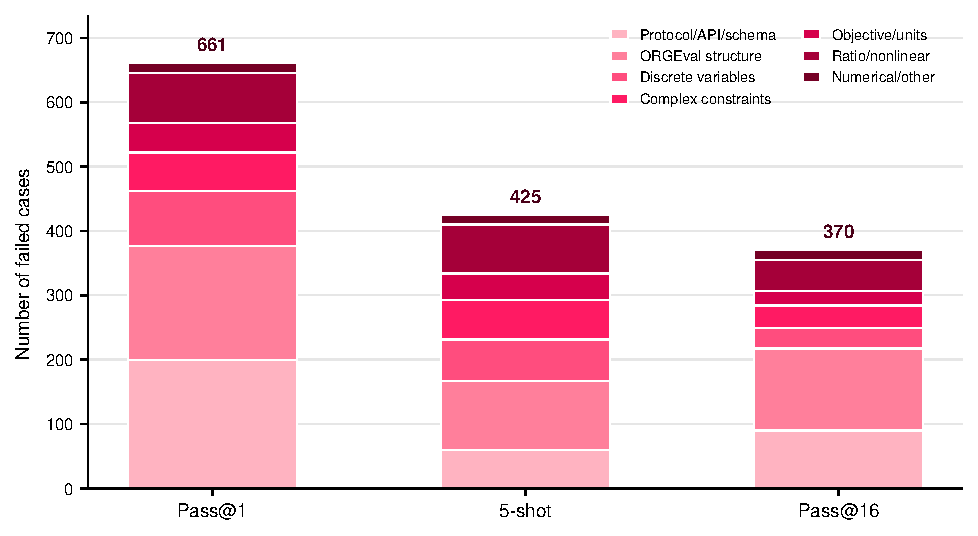
\includegraphics[width=0.92\linewidth]{figures/base_error_family_bars.pdf}
\caption{Stacked error-family counts of the original checkpoint under Pass@1,
5-shot, and Pass@16. The bar heights show total failed cases, while the colored
segments show how the failure composition changes. 5-shot sharply reduces
protocol/API/schema failures; Pass@16 reduces total failures but leaves a large
structural ORGEval segment.}
\label{fig:base_error_family_bars}
\end{figure}

\subsubsection{Inference-Setting Shift}

The distribution shift across inference settings separates promptable
behavioral failures from deeper modeling failures. Under Pass@1, the checkpoint
produces 661 failures, with protocol/API/schema errors forming the largest
family: 199 cases, or 30.1\%. This is the raw evaluator-facing failure
surface of the original checkpoint. Moving to 5-shot reduces failures to 425
and cuts protocol/API/schema errors to 59 cases, showing that many code-only
contracts, Gurobi idioms, and schema-handling habits are already latent and can
be activated by demonstrations. Moving to Pass@16 further reduces total
failures to 370 and improves value-based benchmarks, but structural ORGEval
errors become the largest remaining family, 127 cases or 34.3\%. Thus,
additional sampling can retrieve more numerically correct solutions, but it
does not reliably choose the canonical variable--constraint graph.

The same observations can be read as a training-oriented failure taxonomy.
Below, the failure types are ordered by their overall share among the 1,456
scanned failed cases. This paragraph-level view separates failures that mainly
block the evaluation interface from failures that expose missing OR modeling
priors, while keeping the representative cases and training implications tied
to concrete samples.

\paragraph{Canonical structure mismatch under ORGEval (28.3\%).}
This is the largest failure type in the scan and the most important structural
problem. In the pharmaceutical blending cases \texttt{BENCH4OPT\_0/1}, the
generated LP can be executable, but it fails variable-count or
constraint-count checks because the model uses a non-reference variable or
constraint family. \texttt{BENCH4OPT\_12} further shows that even when variable
and constraint counts match, the WL graph can still be wrong because the
constraint--variable connections differ. These failures are important because
solver success or a plausible objective value is not enough for ORGEval: the
model must produce the canonical LP graph. CPT is needed for domain templates
such as blending, scheduling, and flow; SFT is needed to align these templates
with benchmark-facing variable and constraint families.

\paragraph{Output protocol, syntax, API, and schema failures (23.9\%).}
This is the most fatal evaluation-interface problem. In \texttt{BENCH4OPT\_4},
a capital-budgeting problem, the Pass@1 response adds a markdown code fence in
a code-only target, causing a syntax failure before model construction. In
\texttt{BENCH4OPT\_176}, a nurse-scheduling problem, a string shift label is
used to index a list of requirements, triggering a schema/indexing runtime
error. These cases show that the checkpoint may have usable OR reasoning
internally but fail to expose it through the required program interface.
Non-executable code is scored as zero regardless of whether the mathematical
idea is correct, so this family can severely mask the checkpoint's real OR
capability. It primarily motivates SFT: code-only contracts, verified Gurobi
APIs, and schema-safe templates must become stable Pass@1 behavior.

\paragraph{Discrete variable semantics (12.5\%).}
NL4OPT 15 is a staffing problem that asks for numbers of senior and young
workers. The model encodes the worker counts as \texttt{GRB.CONTINUOUS} and
returns the LP relaxation value 28125.0 instead of the integer optimum
28250.0. The same relaxation persists under 5-shot and Pass@16, showing that
prompting and sampling do not reliably recover the missing integrality prior.
This is a core OR semantics problem: the model understands many constraints,
but fails to map countable business entities to integer or binary variables.
CPT should strengthen countable-entity priors, while SFT should provide
explicit integer/binary Gurobi demonstrations for workers, trips, batches,
vehicles, assignments, and selections.

\paragraph{Loss/yield-driven conservation constraints (10.8\%).}
\texttt{BENCH4OPT\_2} is a water-distribution network-flow problem with
capacity, cost, evaporation rate, and node demand. The Pass@1 model solves an
LP but mixes evaporation into both cost and conservation in a way that returns
265.58 instead of 531.15. 5-shot and Pass@16 recover the correct value,
showing that the template is promptable but not stable. This represents
complex constraint semantics rather than mere code generation. Loss, yield,
shrinkage, and evaporation determine where conservation equations change and
whether costs or delivered quantities change. CPT should teach these domain
patterns, while SFT should distill promptable templates into stable
data-separated code.

\paragraph{Ratio, unit, and total-quantity coupling (7.4\%).}
OptiBench 6 is a logistics investment problem where route-optimization
investment reduces per-truck delivery cost and total investment must not exceed
total savings. Pass@1 and Pass@16 recognize the bilinear relation but mishandle
investment units and total savings; 5-shot removes the truck-count multiplier
from the savings constraint. This failure corrupts the economic meaning of an
optimization model while still producing plausible algebra. Ratio, ROI,
average-cost, percentage, and efficiency expressions require the model to
distinguish per-unit quantities, totals, denominators, and scaling units. CPT
should broaden this semantic prior, while SFT can teach verified formulations.

\paragraph{Solver-compatible nonlinear reformulation (6.4\%).}
OptiBench 13 asks for the closest feasible rescue point on a parabolic
boundary. The Pass@1 solution writes a fourth-order distance objective directly
into Gurobi and triggers an ``objective must be linear or quadratic'' error.
5-shot and Pass@16 avoid the build error but still return the wrong distance,
which means the missing piece is not just API syntax but nonlinear
reformulation knowledge. This blocks a whole class of mathematically valid OR
tasks. The model must know when to introduce auxiliary variables, when to use
quadratic/nonconvex/general constraints, and when analytic simplification is
required. CPT is the main lever; SFT hardens the verified Gurobi patterns.

This taxonomy explains why the setting-wise distribution motivates both
training stages. The Pass@1 distribution is dominated by protocol/API/schema
and structural failures, so SFT is needed to make code-only generation, Gurobi
API usage, objective extraction, and JSON-style data access stable without
in-context demonstrations. The 5-shot distribution shows which failures are
distillable: markdown fences, several API mistakes, and some common
formulation templates improve sharply once examples are present. This directly
motivates verified SFT and few-shot distillation. However, the residual
5-shot errors concentrate in integer semantics, complex constraints,
ratio/nonlinear modeling, and ORGEval structure, which are not just output
habits. They require CPT to broaden the model's OR formulation priors before
SFT can reliably elicit them.

The Pass@16 distribution adds a different lesson. Because total failures fall
from 425 to 370 and value-based accuracies improve, the original sampling
distribution already contains many recoverable correct programs; this supports
verifier-guided SFT and rejection-sampled distillation from Pass@\(N\) outputs.
But Pass@16 leaves more structural ORGEval failures than 5-shot, both in
absolute count (127 vs. 108 grouped structural errors) and in share
(34.3\% vs. 25.4\%). Sampling therefore improves search over solutions without
enforcing the canonical LP graph. This is the key bridge to CPT plus SFT: CPT
shifts the model toward OR-native structural priors, while SFT turns those
priors into benchmark-facing, executable, and aligned outputs.

\subsubsection{Two-Stage Training Adaptation: Why Both CPT and SFT}

In large language model pipelines, continual pre-training serves as a knowledge-infusion stage---adapting the model to a domain through self-supervised learning on unlabeled corpora~\citep{gururangan2020dontstop, ke2025demystifying, siriwardhana2024domain}---while instruction tuning acts as a behavior-shaping stage~\citep{ouyang2022training, wei2022finetuned, sanh2021multitask} that aligns the model with human intent via supervised learning on instruction-response pairs. The core distinction is that continual pre-training determines what the model knows, and instruction tuning controls how it responds. Their relationship is one of foundation and activation: continual pre-training first builds a domain-informed knowledge base, and subsequent instruction tuning elicits it as coherent, instruction-following behavior~\citep{yang2025main, jindal2024balancing, jiang2025mix, zhang2025adept}. Only this cascaded synergy yields models that are both domain-proficient and reliably usable.

The setting-wise diagnosis gives a clean division of labor. CPT targets
knowledge acquisition: OR terminology, standard formulation patterns,
solver-aware nonlinear reasoning, fractional and efficiency modeling,
data-structure grounding, and structural modeling priors. These are the
failure modes that persist even when examples or multiple samples are added:
integer-domain semantics, nonlinear reformulation, ratio modeling, missing
constraint families, and canonical LP graph structure.

SFT targets solver-oriented behavioral alignment. It should teach the model
to obey code-only and LP-writing contracts, avoid markdown fences, use
verified Gurobi APIs, map JSON/list/dict data safely into index sets, extract
objective values with the right units, and reproduce benchmark-facing
canonical formulations. The 5-shot improvements show that many of these
habits are already promptable; SFT converts that prompt dependence into
stable Pass@1 behavior. The Pass@16 improvements show that correct solutions
often exist in the sampling distribution; verifier-guided distillation can
convert those retrieved samples into parameterized competence. The remaining
structural and modeling failures explain why this SFT stage should be built
on top of OR-oriented CPT rather than replacing it.

\subsection{OR-Oriented Continued Pre-Training}
\label{subsec:or_cpt}

The original-checkpoint analysis shows that DeepSeek-V4-Flash already contains
a useful OR modeling core, especially on standard LP and MILP templates, but
its remaining errors concentrate on variable-domain semantics,
solver-compatible nonlinear reformulation, ratio- and efficiency-based
modeling, complex constraint construction, and structural equivalence. These
failure modes indicate that the next stage should not only teach the model to
follow benchmark protocols, but also strengthen its prior over OR-domain
concepts, mathematical-programming structures, and solver-aware modeling
patterns. We therefore use CPT as the knowledge-acquisition stage in the
OR-oriented post-training workflow, following the domain-adaptive
pre-training paradigm for adapting language models to specialized
distributions~\citep{gururangan2020dontstop,chen2026continual_learning_llm}.

In this stage, the model is further trained on a domain-dominant mixture built
around solver-verified OR documents. The design is guided by the capability
gaps observed in the original checkpoint: integer and binary variable
semantics motivate broader exposure to countable-entity formulations;
nonlinear and ratio-based failures motivate solver-aware reformulation data;
and ORGEval structural mismatches motivate data that preserves canonical
variable families, constraint families, and constraint--variable connections.
Following this principle, our CPT workflow centers on an OR-CPT data engine
that converts parameterized optimization generators into traceable,
business-oriented, and executable modeling documents. The resulting CPT stage
serves as a bridge between data construction and SFT: it expands the model's
OR-domain modeling distribution before SFT aligns the checkpoint with verified
Gurobi code, strict output contracts, and benchmark-specific formulation
styles~\citep{jiang2025mix}.

\subsubsection{OR-CPT Data Construction and Domain-Dominant Mixture}
\label{subsubsec:cpt_data_construction}

The core of our CPT data construction is the OR-CPT Data Engine, a
solver-verified bidirectional synthesis workflow that converts structured
optimization instances into natural-language modeling documents, as illustrated
in Figure~\ref{fig:or_cpt_pipeline}. The workflow
targets the capability gaps observed in the original-checkpoint analysis,
including variable-domain ambiguity, weak parameter grounding, incomplete
constraint construction, nonlinear or ratio-based modeling failures, and
structural mismatch under ORGEval-style evaluation. Each accepted CPT document
is traceable to a generated optimization instance, an independently verified
solver reference, and a checked forward modeling result.

The workflow starts from parameterized optimization instance generators. Each
generator specifies the decision variables, objective, constraints, numerical
parameters, and task-specific structure of an optimization family. The current
generator registry covers assignment, scheduling, facility location, network
flow, production planning, lot sizing, routing, covering, transportation,
portfolio optimization, and revenue management. For each instance, the engine records structured metadata, including task family, generator identity, concept tags, difficulty label, generation parameters, and canonical mathematical signature. This metadata is used for corpus sampling, auditing, and concept-level analysis, but is not exposed as model-facing CPT text. We also maintain separation between the data-generation assets and the ORGEval evaluation assets: no ORGEval reference formulation, canonical LP graph, or evaluator-side template is reused when rendering CPT documents. The intended overlap is at the level of broad OR problem families and modeling concepts, rather than at the level of shared canonical templates or instance provenance.


Each generated instance is independently executed with Gurobi to obtain a
reference solver status, objective value, variable assignment, and constraint
diagnostics. The engine then applies instance-level quality filters to remove
unstable or low-value samples, including infeasible instances, degenerate
all-zero solutions, duplicated parameter configurations, duplicated solution
signatures, and weak optimization trade-offs. This solver-grounded filtering
step provides the mathematical anchor for the synthetic corpus and improves the
quality of the subsequent natural-language modeling documents.

\begin{figure}[t]
  \centering
  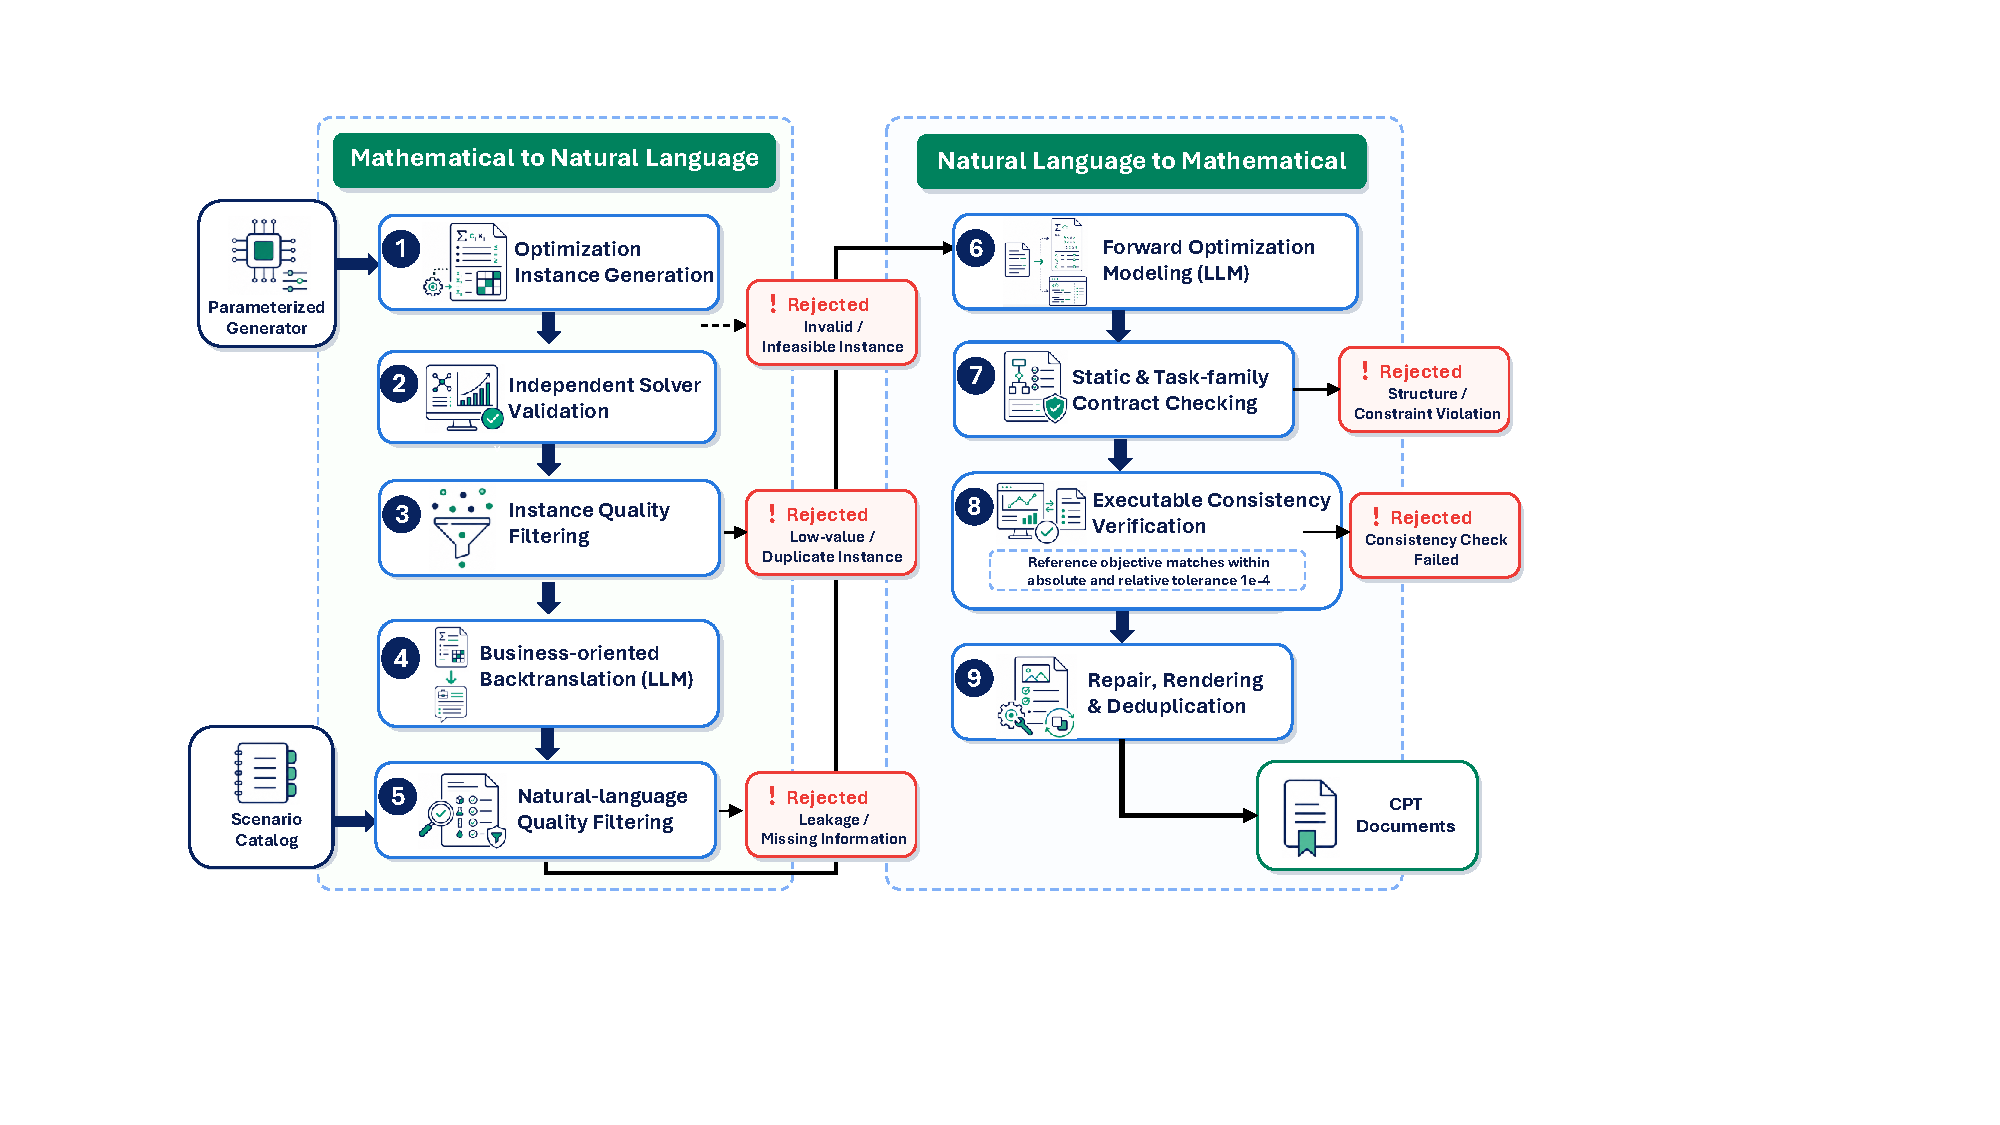
\includegraphics[width=1.0\textwidth]{figures/data_engine.pdf}
  \caption{Pipeline of OR-CPT data construction. Parameterized optimization generators produce structured instances, which are verified with Gurobi, rendered into business-oriented problem statements, reconstructed into executable formulations, and filtered by contract checks, solver execution, and objective-value agreement before export.}
  \label{fig:or_cpt_pipeline}
\end{figure}

After solver validation, the structured instance is converted into a
business-oriented natural-language problem. A scenario catalog controls the
industry background, organization type, planning horizon, entity naming style,
units, and narrative perspective. Deterministic leakage checks prevent the
problem statement from exposing the optimal objective value, solver status,
implementation code, or other answer-related artifacts. This step turns a
mathematical instance into a realistic modeling prompt while preserving the
underlying optimization structure.

The second direction of the workflow performs forward modeling from the
generated natural-language problem. Given only the problem statement, a model
produces decision variables, objective functions, constraints, modeling
explanations, and executable Gurobi code. The generated answer is checked by
static rules and task-family contracts. For example, facility-location samples
are expected to connect facility-opening variables with assignment variables,
network-flow samples should contain flow-conservation constraints, and
scheduling samples should preserve assignment, coverage, and capacity
structures. The reconstructed Gurobi program is then executed independently
and compared with the solver reference from the original structured instance.
A sample is accepted only when the program reaches a valid solver status and
its objective value matches the reference solution within the verification
tolerance. Recoverable failures are repaired with structured solver feedback,
and accepted documents are rendered and deduplicated before export.

This bidirectional design gives the synthetic CPT corpus three useful
properties. It is scalable because new data can be produced from parameterized
OR generators across many task families. It is verifiable because each
accepted document is tied to solver execution and reference-objective
agreement. It is structurally informative because the workflow preserves the
connection among natural-language requirements, variable families, constraint
families, solver code, and objective values. These properties make the OR-CPT
Data Engine the main source of solver-grounded modeling signal in our CPT
stage.

The complete CPT corpus combines these solver-verified synthetic documents
with collected OR-domain resources. The collected portion covers optimization
modeling, mathematical reasoning, and solver-oriented problem solving,
including OptMATH~\citep{optmath2025}, ReSocratic and
OptiBench~\citep{yang2025optibench}, Text2Opt-Bench~\citep{gao2026text2opt},
OR-Instruct~\citep{orlm}, NLP4LP~\citep{optimus2024}, ORQA-derived
data~\citep{orqa,synthetic_orqa_2025}, and MAMO~\citep{huang2024mamo}. We
also include OR research papers, official Gurobi modeling examples, and
textbook-style materials to increase coverage of formal modeling conventions,
solver usage, and domain terminology
~\citep{frontieror2026,gurobi_modeling_examples,lownes2024or}. All collected
resources are converted into a unified CPT document format and processed
through source-aware cleaning, formatting, and deduplication. At the current
stage, the OR data pool contains approximately 100K samples, which serve as
the corpus inventory for CPT sampling.

We adopt a domain-dominant mixture strategy in which OR documents provide the
main adaptation signal. Mathematical, code, and general English corpora are
included as supporting components. The mathematical component is drawn from
selected AutoMathText-V2 subsets~\citep{automathtext_v2}, following the
AutoMathText data-selection methodology~\citep{automathtext}, and supports
symbolic formulation, derivation, and multi-step reasoning. The code component
is drawn from NVIDIA Nemotron pretraining data releases, including
scientific-coding data associated with the Nemotron Nano series and
code-concept data associated with Nemotron 3 Super
~\citep{nvidia2025nvidianemotronnano2,nvidia2026nemotron3superopen}, and
supports procedural reasoning, solver-oriented implementation, and robust code
generation. The general English component uses Ultra-FineWeb-L3, derived from
Ultra-FineWeb under the UltraData tiered data management framework
~\citep{ultra_fineweb,ultra_data_tiered}, to maintain broad language
comprehension and generation quality. In this mixture, OR data strengthens
formulation semantics and structural modeling priors, mathematical data
supports reformulation and symbolic reasoning, code data supports executable
solver implementation, and general English data stabilizes broad language
capability. The exact sampling allocation is treated as a recipe-level
parameter and reported with the training configuration.

\subsubsection{Training Execution in the Ascend Ecosystem}
\label{subsubsec:cpt_training_execution}

We execute OR-oriented CPT within the Ascend software ecosystem, using
MindSpeed and TorchTitan-NPU as two implementation routes. Both routes follow
the same autoregressive training objective, OR-oriented data interface,
monitoring protocol, and checkpoint-evaluation workflow. This design keeps the
CPT recipe consistent across different Ascend training abstractions, so that
data construction, optimization behavior, and downstream validation remain
comparable.

The execution setup is configured around the main requirements of
DeepSeek-V4-Flash CPT. Long-context training is supported through context
parallelism, which is important for OR documents that contain business
descriptions, mathematical formulations, solver traces, and multi-step
modeling explanations. Sparse MoE execution is supported through expert
parallelism, token dispatch, and grouped expert computation. The training stack
also supports model-specific attention and MoE operator paths, MTP training,
activation recomputation, and memory-aware optimizer execution. These
capabilities provide the execution basis for full-parameter CPT while keeping
the model architecture and language-modeling objective unchanged.

The broader Ascend system design, including cluster organization, collective
communication, operator optimization, runtime monitoring, and fault recovery,
is reported in Section~\ref{sec:train_infra}. Here, the training execution
serves as the substrate for the OR-oriented CPT recipe. During CPT, we monitor
loss dynamics, learning-rate progression, gradient norms, numerical stability,
throughput, memory behavior, and iteration stability. These signals are used to
identify stable candidate checkpoints for intermediate evaluation and
subsequent SFT. Recipe-level settings, including sequence length, batch size,
learning-rate schedule, parallelism degrees, optimizer configuration, and
memory-saving mechanisms, are summarized in
Appendix~\ref{app:post_training_recipes}.

\subsubsection{Checkpoint Selection and CPT-to-SFT Transfer Validation}
\label{subsubsec:cpt_checkpoint_selection}

CPT checkpoints are selected according to their value as SFT initializations.
We evaluate intermediate checkpoints with three complementary signals:
OR-domain likelihood, general-capability retention, and downstream OR transfer.
The OR likelihood signal is measured on a held-out OR validation set that is
disjoint from the CPT training mixture. It provides an early indication of
whether the checkpoint better models OR terminology, formulation patterns, and
solver-oriented documents. General validation loss and representative
general-capability benchmarks are tracked in parallel to monitor whether the
checkpoint preserves the mathematical, coding, and language abilities needed
for later instruction tuning.

We further evaluate selected checkpoints on OR downstream benchmarks. These
benchmarks cover different aspects of optimization modeling: NL4OPT emphasizes
natural-language-to-formulation ability, OptiBench evaluates broader
optimization problem understanding, B4O-Feasible measures solver-facing
feasibility behavior, and B4O-ORGEval tests structural modeling quality through
a stricter formulation-level evaluation. This benchmark set allows us to check
whether improvements in OR-domain likelihood translate into measurable gains in
modeling, implementation, and structural-equivalence behavior.

Since CPT is designed as a preparation stage for SFT, its most important
evaluation is matched transfer validation. We compare two controlled training
routes:
\begin{align}
\text{Route A:}\quad & \text{Original Checkpoint} \rightarrow \text{SFT}, \\
\text{Route B:}\quad & \text{Original Checkpoint} \rightarrow \text{CPT} \rightarrow \text{SFT}.
\end{align}
The SFT dataset, optimizer configuration, update steps, and evaluation protocol
are kept the same between the two routes. As a result, the difference
between the trained models reflects the contribution of CPT as an initialization
stage. For a downstream benchmark \(b\), we define the transfer gain as:
\begin{equation}
\Delta_{\mathrm{transfer}}^{(b)}
=
S_{\mathrm{CPT+SFT}}^{(b)}
-
S_{\mathrm{SFT}}^{(b)} ,
\end{equation}
where \(S_{\mathrm{CPT+SFT}}^{(b)}\) is the score of the model trained through
Route B and \(S_{\mathrm{SFT}}^{(b)}\) is the score of the matched SFT-only
route.

The final checkpoint is selected with a multi-objective criterion. A preferred
checkpoint should reduce OR validation loss, maintain stable optimization
signals during training, preserve general capabilities within the expected
range, and produce positive CPT-to-SFT transfer on the primary OR benchmarks.
This selection procedure connects the CPT stage directly to the later SFT and
experimental analysis: CPT is not only evaluated as a language-modeling
continuation, but as a domain-adaptive initialization whose value is determined
by downstream OR modeling gains under matched training conditions.

% \section{OR-Oriented Continued Pre-Training on Ascend NPUs}
% \label{sec:cpt}

% Post-training large-scale foundation models for domain-specific reasoning
% requires a careful balance between domain adaptation and the preservation of
% general capabilities. In our post-training pipeline, continued pre-training
% is positioned as the knowledge-oriented stage for the OR-oriented
% validation workflow within the DeepSeek V4 model family. Following the
% domain-adaptive continued pre-training paradigm
% ~\citep{gururangan2020dontstop,chen2026continual_learning_llm}, this stage
% updates all trainable parameters under the standard autoregressive language
% modeling objective, using a carefully constructed domain-dominant data mixture
% rather than instruction-response supervision. Its purpose is to increase the
% model's exposure to OR terminology, mathematical structures, modeling
% conventions, solver-oriented documents, and algorithmic reasoning patterns,
% while retaining the mathematical, coding, and general-language capabilities
% needed for downstream task solving.

% This role is distinct from that of supervised fine-tuning. CPT primarily
% serves knowledge acquisition and distributional adaptation, whereas SFT elicits
% the acquired knowledge under instruction-following, code-generation, and
% benchmark-specific output formats. This separation is useful in practice, but
% it also requires CPT checkpoints to be evaluated for their compatibility with
% subsequent SFT, rather than only for standalone language-modeling loss. We
% therefore design the CPT workflow around the same OR capability taxonomy used
% in later SFT and evaluation. This capability-oriented taxonomy informs the
% construction of synthesized OR-domain data, the selection of supporting
% mathematical, code, and general English corpora, the design of intermediate
% validation signals, and the checkpoint interface to SFT. Under this design, CPT
% is treated as a controlled knowledge-acquisition stage that provides a stronger
% initialization for instruction tuning.

% This section describes the CPT stage from four perspectives. We first introduce
% the objective and design principles of OR-oriented CPT, emphasizing its role as
% a full-parameter domain-adaptive training stage. We then describe the
% OR-oriented corpus construction and domain-dominant mixture used in the
% reported experiments, including synthesized OR data and supporting
% mathematical, code, and general English resources. Next, we present the
% Ascend-based implementation through the MindSpeed and TorchTitan-NPU routes,
% together with the training capabilities required by long-context sparse MoE
% models. Finally, we describe the immediate evaluation and checkpoint-selection
% procedure, which combines OR validation loss, general validation signals,
% selected downstream benchmarks, and CPT-to-SFT transfer results to assess
% whether a CPT checkpoint is suitable for subsequent SFT.

% \subsection{CPT Objective and Design Principles}
% \label{subsec:cpt_objective}

% We treat CPT as a full-parameter domain-adaptive continuation of the base
% model under the standard autoregressive language modeling objective. Following
% the domain-adaptive pre-training paradigm, the pre-trained model is further
% exposed to domain-relevant corpora instead of being retrained from scratch
%~\citep{gururangan2020dontstop,chen2026continual_learning_llm}. In our setting,
% this stage is intended to increase the model's exposure to OR terminology,
% mathematical formulations, modeling conventions, and solver-oriented reasoning
% patterns, without directly optimizing instruction-following behavior or output
% style.

% This design distinguishes CPT from subsequent SFT. CPT primarily supports
% knowledge acquisition and distributional adaptation, whereas SFT elicits the
% acquired knowledge under instruction-following, code-generation, and
% task-solving formats. Prior work on continual learning for LLMs distinguishes
% continual pre-training, continual fine-tuning, and continual alignment as
% different stages with different optimization targets and forgetting risks
% ~\citep{chen2026continual_learning_llm}. We therefore use CPT as a controlled knowledge-acquisition stage before SFT. This view is
% also consistent with recent CPT work that separates knowledge learning from
% format or instruction alignment~\citep{jiang2025mix}.

% Our CPT recipe follows a conservative full-parameter adaptation strategy. We do
% not modify the model architecture or introduce task-specific modules. Instead,
% all trainable parameters are updated under the same language modeling
% objective, and the adaptation behavior is controlled primarily through the
% training-data distribution. This reflects the stability--plasticity trade-off
% in continual learning: the model should acquire OR-relevant knowledge while
% retaining previously learned general capabilities. Accordingly, the CPT corpus
% uses a domain-dominant mixture in which OR data provides the main adaptation
% signal, while mathematical, code, and general English data provide supporting
% signals for symbolic reasoning, solver-oriented implementation, and
% general-capability retention. The following subsection describes how this
% principle is instantiated through OR-oriented corpus construction and data
% sampling.

% A useful CPT checkpoint should improve OR-domain adaptation while remaining
% suitable as an initialization for SFT. We therefore evaluate CPT checkpoints
% from both perspectives: OR validation loss and OR-oriented downstream
% benchmarks measure domain adaptation, while general validation signals,
% selected general-capability checks, and matched CPT-to-SFT transfer experiments
% measure retention and SFT compatibility. This evaluation principle follows the
% continual-learning motivation that successful adaptation should improve the
% target domain while limiting degradation on previously acquired capabilities
%~\citep{chen2026continual_learning_llm}.

% \subsection{OR-oriented Data Construction and Mixture Design}

% \paragraph{Corpus composition and sources.}

% The OR corpus combines previously collected and cleaned domain resources with newly synthesized optimization-modeling documents. The collected portion consolidates and reprocesses public resources for optimization modeling, mathematical reasoning, and solver-oriented problem solving, including OptMATH~\citep{optmath2025}, ReSocratic~\citep{yang2025optibench}, Text2Opt-Bench~\citep{gao2026text2opt}, OR-Instruct~\citep{orlm}, NLP4LP~\citep{optimus2024}, ORQA-derived data ~\citep{orqa,synthetic_orqa_2025}, and MAMO~\citep{huang2024mamo}. We additionally incorporate domain text derived from OR research papers, official Gurobi modeling examples, and an operations research textbook ~\citep{frontieror2026,gurobi_modeling_examples,lownes2024or}. These resources are normalized into a common CPT document format and subjected to source-aware cleaning, formatting, and deduplication.

% At the current stage, the OR data pool contains approximately 100K samples. These samples constitute the available corpus inventory at the dataset level and are used to support subsequent CPT data construction and sampling. The reported sample count describes the overall scale of the available corpus and should be distinguished from the token-level sampling proportions applied during CPT.

% The synthesized portion is produced by the OR-CPT Engine, which converts optimization instance generators into scalable, verifiable, and traceable CPT documents. Rather than relying on unconstrained language-model generation, the engine uses independently executed optimization instances and solver outcomes as the source of mathematical reference. The current generator registry contains a broad set of enabled generator profiles spanning multiple OR task families, including assignment, scheduling, facility location, network flow, production planning, lot sizing, routing, covering, transportation, portfolio optimization, and revenue management. Each generated instance is associated with structured metadata, including its task family, generator identity, concept tags, difficulty label, generation parameters, and canonical mathematical signature.

% \paragraph{Bidirectional synthesis and verification.}

% The data construction process is illustrated in
% Figure~\ref{fig:or_cpt_pipeline}. It consists of the following major stages:


% \begin{figure}[t]
%   \centering
%   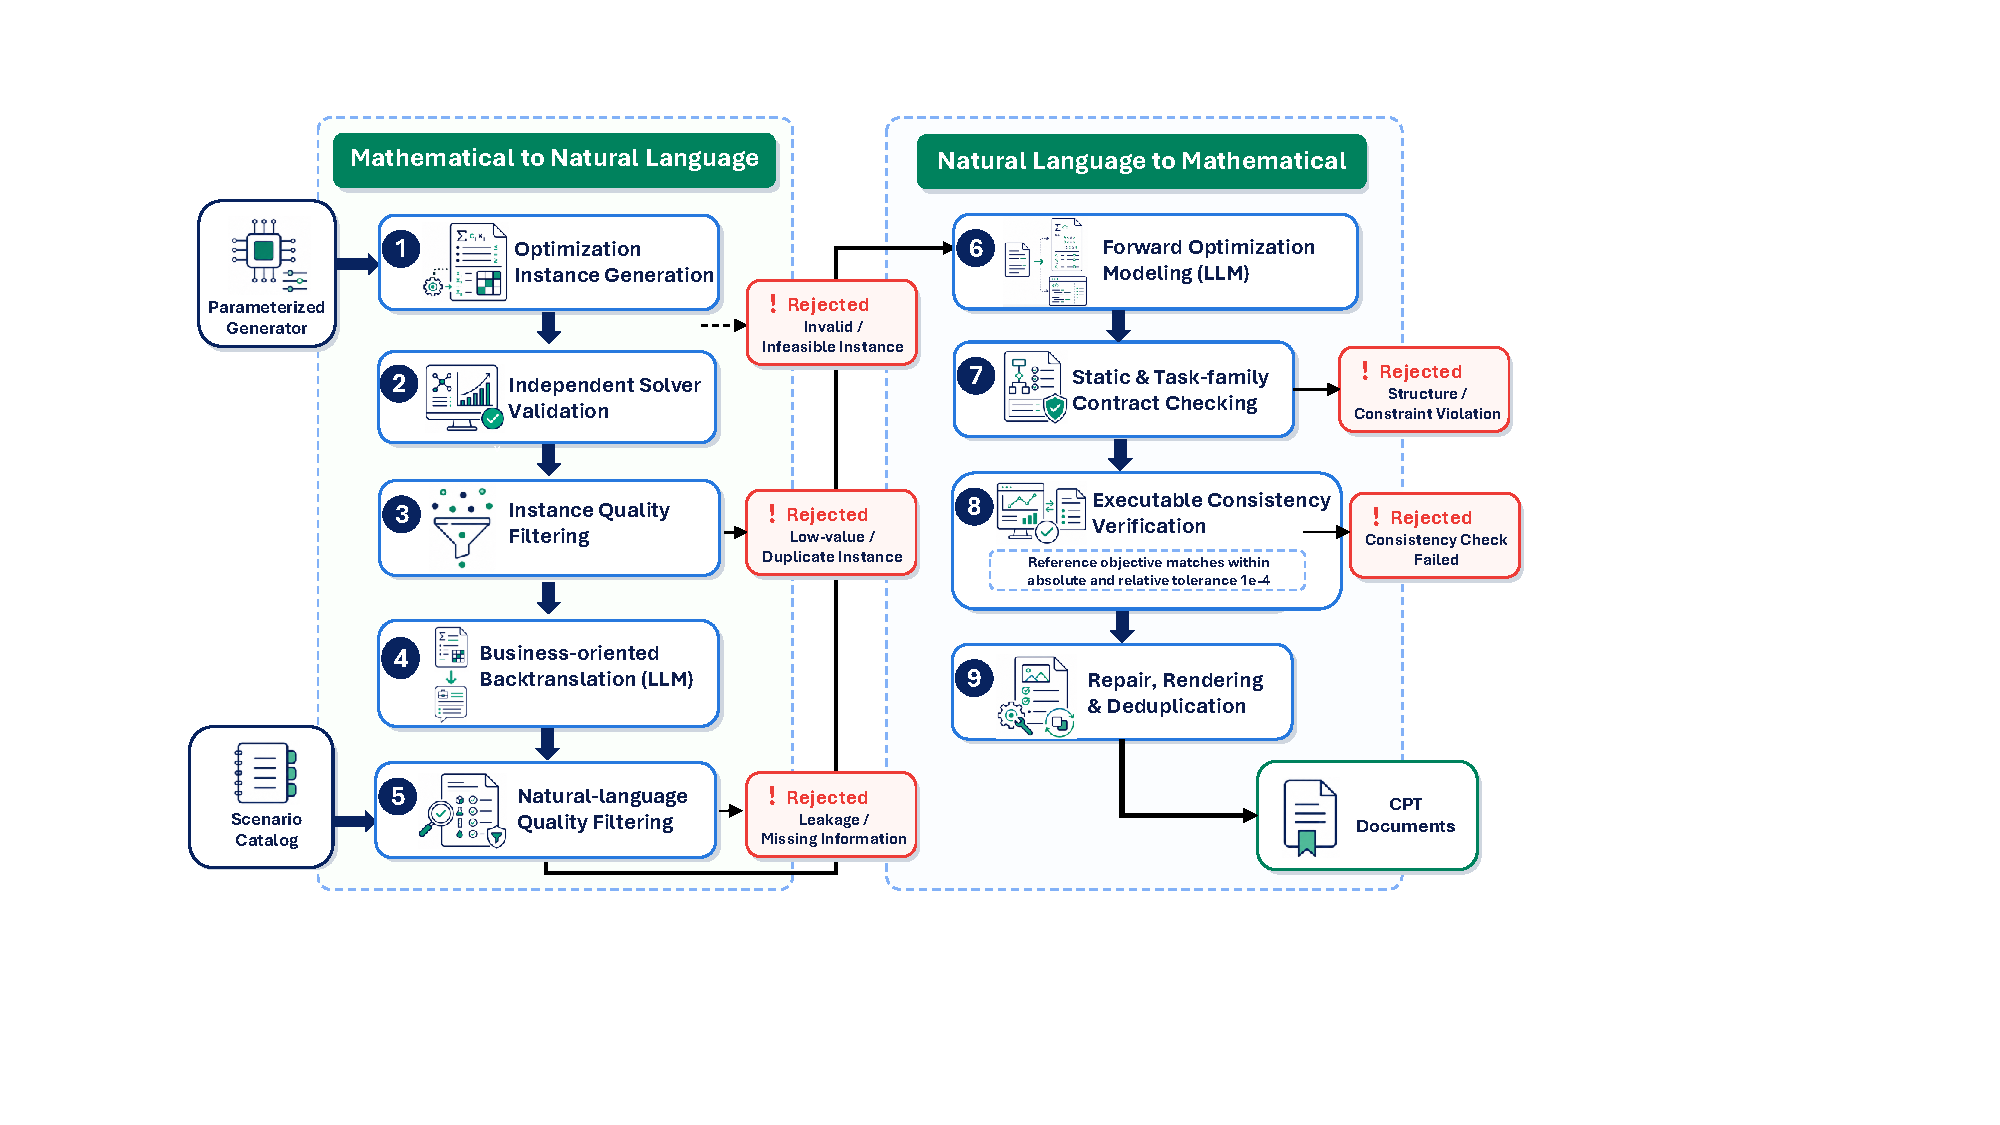
\includegraphics[width=1.0\textwidth]{figures/data_engine.pdf}
%   \caption{The pipeline of CPT data construction.}
%   \label{fig:or_cpt_pipeline}
% \end{figure}

% \begin{enumerate}
% \item \textbf{Optimization instance generation.}
% A parameterized generator produces a structured optimization instance,
% including its variables, objective, constraints, and numerical parameters.

% \item \textbf{Independent solver validation.}
% The instance is independently executed with Gurobi to obtain a reference
% solver status, objective value, variable assignment, and constraint
% diagnostics. Instances that are infeasible, unstable, or incorrectly
% specified are rejected.

% \item \textbf{Instance quality filtering.}
% Solver feasibility alone does not imply training value. We additionally
% check for degenerate all-zero solutions, insufficiently active constraints,
% duplicated parameter configurations, duplicated solution signatures, and
% weak or trivial optimization trade-offs.

% \item \textbf{Business-oriented backtranslation.}
% A language model transforms the mathematical instance into a natural
% language business problem. A scenario catalog controls the industry,
% organization type, business trigger, planning horizon, entity naming style,
% and narrative perspective.

% \item \textbf{Natural-language quality filtering.}
% Deterministic filters check whether the problem statement contains the
% required entities, decisions, quantities, and units. They also prevent
% leakage of the optimal objective value, solver status, implementation code,
% or other answer-related information.

% \item \textbf{Forward optimization modeling.}
% Given only the generated natural-language problem, a language model
% reconstructs the decision variables, objective function, constraints,
% modeling explanation, and executable Gurobi code.

% \item \textbf{Static and task-family contract checking.}
% The generated answer is checked for required Gurobi operations and
% task-specific modeling structures. For example, facility-location problems
% must connect facility-opening variables with service assignments, while
% network-flow problems must contain appropriate flow-conservation
% constraints.

% \item \textbf{Executable consistency verification.}
% The generated Gurobi program is executed independently. A sample is accepted
% only when the program reaches an acceptable solver status and its objective
% value agrees with the reference objective within an absolute and relative
% tolerance of $10^{-4}$.

% \item \textbf{Repair, rendering, and deduplication.}
% Recoverable failures can be passed through a one-step repair procedure using
% structured solver feedback. Accepted samples are rendered into CPT
% documents and deduplicated before export.

% \end{enumerate}

% \paragraph{Supporting data for capability retention and OR-adjacent reasoning.}

% In addition to the OR corpus, we include mathematical, code, and general English data to support capability retention and provide complementary reasoning signals during CPT. The code component is drawn from NVIDIA's Nemotron pretraining data releases, covering scientific-coding data associated with the Nemotron Nano series~\citep{nvidia2025nvidianemotronnano2} and code-concept data released with Nemotron 3 Super~\citep{nvidia2026nemotron3superopen}. For mathematical coverage, we use selected subsets from AutoMathText-V2~\citep{automathtext_v2}, which builds on the AutoMathText data selection methodology~\citep{automathtext}. For general language coverage, we use Ultra-FineWeb-L3, derived from Ultra-FineWeb~\citep{ultra_fineweb} under the UltraData tiered data management framework~\citep{ultra_data_tiered}.

% These supporting corpora serve distinct but complementary purposes. Mathematical data broadens the model's exposure to symbolic formulation, derivation, and optimization reasoning. Code data helps preserve algorithmic and implementation-related patterns, particularly those associated with solver use, procedural reasoning, and structured problem solving. General English data provides a background distribution for maintaining broad language understanding and limiting excessive domain specialization. Together, these corpora support capability retention and OR-adjacent reasoning, while the OR corpus remains the primary source of domain adaptation.

% \paragraph{Domain-dominant mixture strategy.}

% We adopt a domain-dominant sampling strategy in which OR data constitutes a
% large share of the CPT training mixture. The remaining portion is drawn from
% the mathematical, code, and general English corpora described above. This
% allocation concentrates the training signal on OR terminology, formulation
% patterns, and solver-oriented reasoning, while retaining a background
% distribution that supports symbolic reasoning, code generation, and
% general-capability preservation. The exact allocation, including the internal
% proportions of the supporting corpora, is treated as a recipe parameter that
% can be adjusted according to corpus availability, validation losses, and
% downstream evaluation results.

% \subsection{CPT Implementation on Ascend NPUs}
% \label{subsec:cpt_ascend_impl}

% We implement DeepSeek V4 CPT on Ascend NPUs through two parallel software
% stacks, TorchTitan-NPU and MindSpeed. Both routes support full-parameter
% continued pre-training under the same autoregressive objective and compatible
% OR-oriented data interface, while relying on different framework abstractions
% within the Ascend ecosystem. This subsection focuses on the training
% capabilities required by DeepSeek V4 CPT; the CloudMatrix384 cluster
% organization, collective communication infrastructure, and system-level
% optimization are described in Section~\ref{sec:train_infra}.

% The implementation requirements are mainly determined by three properties of
% DeepSeek V4: model-specific attention computation, sparse MoE execution, and
% long-context full-parameter optimization. The attention path requires
% NPU-adapted execution for compressed key-value representations and sparse
% attention operations, while the MoE layers require efficient token dispatch,
% expert-parallel communication, and grouped expert computation. Long-context CPT
% further increases activation memory and communication cost. Accordingly, the
% implementation focuses on four capabilities: model-specific NPU operator
% adaptation, long-context training with context parallelism, scalable MoE
% training with expert parallelism, and memory-aware full-parameter optimization.

% \paragraph{Parallel implementation routes.}
% TorchTitan-NPU provides a PyTorch-native, configuration-driven training route
% for DeepSeek V4 on Ascend NPUs. MindSpeed provides a parallel implementation
% through its native large-scale training abstractions for Ascend clusters. The
% two routes are not required to share identical internal execution graphs, but
% they are aligned at the level of training objective, data interface, major
% parallelism choices, and monitoring protocol. This design allows the same CPT
% recipe to be validated across different software abstractions in the Ascend
% ecosystem.

% \paragraph{Model-specific NPU operator support.}
% Both routes adapt the main DeepSeek V4 computation paths to Ascend NPUs. The
% operator support covers model-specific attention computation and MoE expert
% computation, together with the supporting normalization and positional-encoding
% operations required by the model. These adaptations allow the training workflow
% to execute the dominant attention and expert paths through NPU-aware kernels
% and fused execution patterns, rather than treating the model as a generic dense
% Transformer.

% \paragraph{Long-context and sparse-attention training.}
% The Ascend implementation supports long-context CPT in the 64K-token regime
% through context parallelism. In this setting, attention states and
% sparse-attention metadata must be partitioned and exchanged across
% context-parallel groups. This capability is important for OR-oriented CPT
% because long-form optimization documents, solver traces, modeling explanations,
% and multi-step reasoning data often contain dependencies that would be lost
% under short-context truncation. Communication and computation are overlapped
% where supported by the backend to integrate the long-context attention path
% into the distributed training workflow.

% \paragraph{MoE, MTP, and memory-efficient optimization.}
% The MoE path is supported through expert parallelism, token dispatch, dynamic
% token grouping, and Ascend-optimized grouped matrix multiplication. Tokens
% routed to different experts are reorganized and processed in grouped expert
% batches, reducing the overhead of launching independent expert computations.
% The training stack also supports the multi-token-prediction modules of DeepSeek
% V4. Since CPT updates all trainable parameters, the implementation further uses
% activation recomputation, distributed optimizer execution, and optimizer-state
% swapping to reduce peak memory pressure without changing the model-level
% training objective.

% \paragraph{Monitoring and configuration reporting.}
% During execution, both routes are monitored through shared optimization and
% system-level signals, including loss dynamics, learning-rate progression,
% gradient norms, numerical stability, throughput, MFU, memory behavior, and
% iteration stability. These signals help distinguish optimization instability
% from system bottlenecks and determine whether a run is suitable for continued
% execution, checkpoint evaluation, and subsequent SFT. Selected recipe-level
% settings, including sequence length, batch size, learning-rate schedule,
% parallelism degrees, optimizer configuration, and memory-saving mechanisms, are
% reported in Appendix~\ref{app:post_training_recipes}.

% \subsection{Intermediate Evaluation, Checkpoint Selection, and Transfer Validation}
% \label{subsec:cpt_evaluation}

% Training loss alone is insufficient for selecting CPT checkpoints. A checkpoint may achieve a lower loss on the CPT mixture while overfitting to the domain distribution, amplifying corpus-specific biases, or degrading general capabilities. We therefore evaluate intermediate checkpoints along three complementary dimensions: domain likelihood, general-capability retention, and downstream OR transfer.

% \paragraph{Domain likelihood.}

% We construct a held-out OR language-modeling validation set that is disjoint from the CPT training mixture. For each checkpoint, we report token-level negative log-likelihood and perplexity:

% \begin{equation} \mathrm{PPL}_{\mathrm{OR}} = \exp\left( \frac{1}{N_{\mathrm{OR}}} \sum_{i=1}^{N_{\mathrm{OR}}} \ell_{i}^{\mathrm{OR}} \right), \end{equation}

% where \(N_{\mathrm{OR}}\) denotes the number of validation tokens and \(\ell_i^{\mathrm{OR}}\) is the negative log-likelihood of the \(i\)-th token. A reduction in OR perplexity indicates that the checkpoint better models the distribution of OR documents. However, this metric is treated as a likelihood signal rather than direct evidence of improved optimization modeling or problem-solving capability.

% \paragraph{General-capability retention.}

% To monitor catastrophic forgetting, we evaluate each candidate checkpoint on a separate general-domain validation set and report \(\mathrm{PPL}_{\mathrm{general}}\). We also evaluate representative general-capability benchmarks, including MMLU, GSM8K, C-Eval, and BBH. For a benchmark score \(S\), we define the retention ratio as

% \begin{equation}
% R_{\mathrm{general}}
% =
% \frac{S_{\mathrm{CPT}}}{S_{\mathrm{base}}}.
% \end{equation}

% A ratio close to one indicates that the corresponding capability is largely retained, whereas a substantial reduction indicates potential catastrophic forgetting. In checkpoint selection, we treat a checkpoint as retention-safe only when the degradation in general validation perplexity and representative general benchmark scores remains within a predefined tolerance range.

% \paragraph{OR downstream evaluation.}

% OR downstream benchmarks are used to determine whether lower domain loss translates into improved modeling and reasoning behavior. We evaluate benchmarks that cover complementary aspects of optimization modeling, including NL4OPT for natural-language-to-optimization modeling, OptiBench for broader optimization problem understanding, B4O feasibility evaluation for constraint and feasibility judgment, and B4O-ORGEval for OR-oriented reasoning and generation quality. These benchmarks are not used as replacements for OR perplexity; rather, they provide task-level evidence that complements the language-modeling validation signal.

% \paragraph{CPT-to-SFT transfer validation.}

% Because CPT is used as a preparation stage for downstream instruction tuning, its final utility is evaluated through controlled CPT-to-SFT transfer experiments. We compare two matched routes: 
% \begin{align} \text{Route A:}\quad& \text{Base Model} \rightarrow \text{SFT},\\ \text{Route B:}\quad& \text{Base Model} \rightarrow \text{CPT} \rightarrow \text{SFT}. \end{align} 

% The SFT dataset, optimizer configuration, number of update steps, and evaluation protocol are held constant between the two routes. This design prevents improvements from being incorrectly attributed to CPT when they are caused by different SFT conditions. For a downstream benchmark \(b\), the CPT transfer gain is defined as 
% \begin{equation} \Delta_{\mathrm{transfer}}^{(b)} = S_{\mathrm{CPT+SFT}}^{(b)} - S_{\mathrm{Base+SFT}}^{(b)}. \end{equation}

% Positive transfer gain indicates that CPT provides a better initialization for subsequent SFT under matched training conditions, while negative transfer gain indicates that the CPT stage may introduce distributional bias or interfere with the downstream SFT objective.

% \paragraph{Pareto-style checkpoint selection.}

% % Combining the above dimensions, checkpoint selection is not a single-objective
% % optimization problem. We adopt a Pareto-style criterion: the selected
% % checkpoint should provide meaningful improvement in OR validation loss or
% % downstream benchmarks, demonstrate positive or neutral $\Delta_{\mathrm{transfer}}$
% % under matched SFT conditions, and keep the degradation of general capabilities
% % within an acceptable range. This means we do not automatically select the
% % checkpoint with the lowest training loss or the latest training step, but
% % instead weigh domain-adaptation gains against general-capability retention
% % costs. This principle directly motivates the CPT data mixture design---expanding
% % domain coverage breadth through diverse task families and generator profiles,
% % introducing solver-verified modeling documents to ensure quality, and
% % maintaining an adequate proportion of general-domain data throughout training.

% Combining the above dimensions, checkpoint selection is treated as a multi-objective decision rather than a single-objective optimization problem. We adopt a Pareto-style criterion in which candidate checkpoints are compared jointly in terms of domain adaptation, downstream transfer, and general-capability retention. A selected checkpoint should provide a meaningful reduction in OR validation loss or improvement on OR downstream benchmarks, demonstrate positive or at least non-negative CPT-to-SFT transfer on primary evaluation tasks under matched SFT conditions, and keep the degradation of general capabilities within a predefined acceptable range.

% This criterion prevents us from automatically selecting the checkpoint with the lowest training loss or the latest training step. Instead, checkpoint selection balances domain-adaptation gains against the cost of possible capability regression. It also motivates the CPT data mixture design: broadening OR domain coverage through diverse task families and generator profiles, introducing solver-verified modeling documents to improve data quality, and maintaining an adequate proportion of general-domain data throughout CPT to reduce forgetting.

% \section{Supervised Fine-Tuning}

% Following the continued pre-training (CPT) phase, the base model possesses an enhanced capacity for domain-specific knowledge but inherently lacks the behavioral alignment required to process complex instruction formats and interactive constraints. In this work, we employ Supervised Fine-Tuning (SFT) to bridge this gap between raw text generation and task-specific alignment, focusing extensively on automating optimization modeling tasks as reviewed by ~\citep{10.24963/ijcai.2025/1192}. The primary objective of this stage is to train the model to systematically translate natural language descriptions of operations research problems into formal, solver-ready symbolic formulations. This process requires the model to precisely extract and declare decision variables, mathematically define objective functions, and formulate rigorous equality and inequality constraints.

% To achieve this capability transformation, we design an industrialized data curation and synthesis pipeline inspired by modern post-training paradigms . Because standard human-annotated datasets lack the scale and precision necessary to cover the diverse mathematical structures of optimization problems, we develop an automated framework to generate high-fidelity, verified training trajectories. Each synthetic sample explicitly breaks down the model-building process into intermediate reasoning steps, enforcing a standardized and interpretable output layout. During training, the model is optimized using a standard cross-entropy loss. To ensure gradient stability and maximize alignment efficiency, the loss is computed exclusively on the target response tokens—representing the reasoning paths and final mathematical formulations—while the loss on the prompt and system formatting tokens is strictly masked during the backward pass (Meta, 2024). Through this combined approach of rigorous behavior mapping and structured data injection, the model effectively elicits its mathematical capabilities without destabilizing its foundational general-domain performance.

% \subsection{Alignment Objectives for Optimization Modeling}

% \subsection{Data Curation and Synthesis Pipeline}

% \subsection{Chain-of-Thought Formulation and Output Standardization}

% \subsection{Training Infrastructure and Hyperparameters}







% % chapter 4
% \section{Data-Efficient Supervised Fine-Tuning for Operations Research}
% \label{sec:sft}

% We conduct supervised fine-tuning for DeepSeek-V4-Flash~\citep{xu2026deepseek} on operations research modeling tasks. The goal is to adapt the model from general instruction following to solver-oriented mathematical programming, with emphasis on benchmarks such as NL4OPT, OptiBench, and Bench4Opt. Unlike general code-generation tasks, OR modeling evaluation does not only check whether the generated program can be executed. It also evaluates natural-language semantic understanding, variable-type selection, objective and constraint construction, correct use of Gurobi-style APIs, external data loading, answer-format contracts, and the equivalence of abstract modeling structures.

% Since large-scale SFT data in the OR domain is scarce, heterogeneous in format, and uncertain in quality, we follow the idea of iterative self-distillation methods such as ReSocratic-style data construction~\citep{yang2025optibench}. The ReSocratic framework generates diverse and reliable optimization data through reverse Socratic synthesis, incrementally building formatted optimization demonstrations before back-translating them into natural language questions~\citep{zhang2025scoder}. More broadly, self-distillation has emerged as a powerful paradigm for bootstrapping high-quality synthetic training data~\citep{lee2026self}, and iterative data synthesis with structured validation has proven particularly effective for optimization modeling tasks~\citep{wu2025training}. For OR-domain SFT data, we adopt a DeepSeek-V4-Flash~\citep{xu2026deepseek} cyclic self-distillation method to construct three training-data scales: 3K, 10K, and 50K. Based on the comparative experiments reported in Section~\ref{subsec:sft_training_cleaning}, we choose the 10K-scale data as the basis for further cleaning and enhancement. The final SFT design therefore focuses not only on scaling synthetic data, but also on improving the correctness, contract awareness, and learnability of the distilled samples.

% \subsection{Solver-Oriented SFT Objective}
% \label{subsec:sft_objective}

% The SFT stage is designed to train the model to form stable optimization-modeling habits. Recent work has established supervised fine-tuning as a critical foundation for equipping LLMs with optimization reasoning capabilities~\citep{orr1}, and the effectiveness of SFT for OR modeling has been demonstrated across multiple frameworks~\citep{xiao2026deepor}. In particular, the model should identify sets, parameters, variables, objectives, and constraints; correctly read structured data files; use Gurobi-style Python APIs to build and solve models; and, when required, write LP files without solving them. The target response is therefore not a simple numerical answer, but a structured modeling trajectory that connects natural-language understanding, mathematical formulation, and solver-facing implementation.

% Given an instruction prompt $x$ and a target response $y=(y_1,\ldots,y_T)$, the SFT stage optimizes the standard autoregressive cross-entropy loss over the response tokens:
% \begin{equation}
% \mathcal{L}_{\mathrm{SFT}}
% =
% -\frac{1}{T}
% \sum_{t=1}^{T}
% \log p_{\theta}(y_t \mid x, y_{<t}).
% \end{equation}
% The loss on prompt, system, and formatting tokens is masked, so that gradient updates are applied only to the target response. This design encourages the model to learn the desired reasoning trajectory, mathematical formulation, and solver implementation, while avoiding unnecessary optimization on fixed prompt templates.


% chapter 4
\subsection{Data-Efficient Supervised Fine-Tuning for Operations Research}
\label{sec:sft}

We conduct supervised fine-tuning for DeepSeek-V4-Flash on operations research modeling tasks. The goal is to adapt the model from general instruction following to solver-oriented mathematical programming, with emphasis on benchmarks such as NL4OPT, OptiBench, and Bench4Opt. Unlike general code-generation tasks, OR modeling evaluation does not only check executability. It also evaluates natural-language semantic understanding, variable-type selection, objective and constraint construction, Gurobi-style API usage, external data loading, answer-format contracts, and structural equivalence of mathematical formulations.

Since large-scale SFT data in the OR domain is scarce, heterogeneous, and uncertain in quality, we adopt a DeepSeek-V4-Flash cyclic self-distillation method inspired by iterative data-construction frameworks such as ReSocratic-style synthesis~\citep{yang2025optibench,zhang2025scoder}. More broadly, self-distillation has been shown to be effective for bootstrapping high-quality synthetic data~\citep{lee2026self}, especially when combined with structured validation for optimization modeling tasks~\citep{wu2025training}. We construct three training-data scales, namely 3K, 10K, and 50K. Based on the comparative experiments reported in Section~\ref{subsec:sft_training_cleaning}, we choose the 10K-scale data as the basis for further cleaning and enhancement. The final SFT design therefore focuses not only on scaling synthetic data, but also on improving the correctness, contract awareness, and learnability of the distilled samples.

\subsubsection{Solver-Oriented SFT Objective}
\label{subsec:sft_objective}

The SFT stage is designed to train the model to form stable optimization-modeling habits. The model should identify sets, parameters, variables, objectives, and constraints; correctly read structured data files; use Gurobi-style Python APIs to build and solve models; and, when required, write LP files without solving them. The target response is therefore not a simple numerical answer, but a structured modeling trajectory that connects natural-language understanding, mathematical formulation, and solver-facing implementation. This follows recent findings that supervised fine-tuning is an important foundation for equipping LLMs with optimization reasoning and modeling capabilities~\citep{orr1,xiao2026deepor}.

Given an instruction prompt $x$ and a target response $y=(y_1,\ldots,y_T)$, the SFT stage optimizes the standard autoregressive cross-entropy loss over the response tokens:
\begin{equation}
\mathcal{L}_{\mathrm{SFT}}
=
-\frac{1}{T}
\sum_{t=1}^{T}
\log p_{\theta}(y_t \mid x, y_{<t}).
\end{equation}
The loss on prompt, system, and formatting tokens is masked, so that gradient updates are applied only to the target response. This encourages the model to learn the desired reasoning trajectory, mathematical formulation, and solver implementation, while avoiding unnecessary optimization on fixed prompt templates.






% \subsection{Self-Distilled OR Modeling Data}
% \label{subsec:sft_dataset_construction}

% We construct a self-distillation data-production pipeline for operations research and mathematical programming modeling tasks. A batch of high-quality modeling QA samples or evaluation samples is first abstracted into an operational modeling intermediate representation. Then, the large model generates new modeling structures, new problem statements, and new standard answers under controlled conditions. Finally, automatic validators filter these samples into SFT data that can be used for supervised fine-tuning.

% We divide the data-production process into several verifiable stages. First, structured modeling semantics are extracted from the original samples. Then, new synthetic IRs are generated. Next, the synthetic IRs are rendered into problems with different styles. After that, answers are generated according to the response specification of each target. Finally, the code is executed or the LP file is checked. Only samples that pass the automatic quality gate are included in the final SFT dataset. The core of this process is to convert the structural requirements, engineering requirements, and format requirements of optimization modeling tasks into training-data specifications, so that the model can learn a standard, complete, and executable mathematical-programming modeling style.

% The input of the whole pipeline is a set of seed samples. Seed samples refer to original problems, reference answers, reference code, data files, or LP files from high-quality modeling QA data. These seed samples are not directly exported as final training samples. Instead, they are used as references for problem types, modeling structures, and target response specifications. They are organized into three problem modes: DP, DT, and DPS. DP, namely Data in Problem, means that the data is directly written in the problem statement. DT, namely Data in Table, means that the data is provided in a tabular form such as a Markdown table. DPS, namely Data-Problem Separate, means that the problem statement and data files are separated, for example, \texttt{data.json}, \texttt{instance.json}, and CSV files.

% \subsection{Intermediate Representations and Data Flywheel}
% \label{subsec:sft_ir_flywheel}

% We introduce three levels of intermediate representations to make the self-distillation process controllable and auditable. This layered approach to data construction mirrors the progressive synthesis strategies explored in recent work on optimization data generation~\citep{yang2025optibench}~\citep{wu2025training}, where intermediate representations enable systematic control over problem complexity and structural diversity. The first level is L1 Canonical IR, which is a conservative normalized record of the original sample. It does not attempt to fully reconstruct all mathematical formulas, but stably records the source path, target contract, data interface, reference-file status, static code features, risk labels, and objective-function hints. The role of L1 is to unify initial samples with heterogeneous formats into a structured basis that can be read by the subsequent pipeline.

% The second level is L2 Semantic IR. Semantic IR is a semantic modeling representation extracted from seed samples. It is closer to the mathematical-programming problem itself than L1, and describes the objective function, sets, parameters, variables, constraints, data interface, and potential risks. The significance of the L2 stage is to abstract the knowledge of how the problem should be modeled from the concrete problem statement, so that subsequent generation does not rely on superficial rewriting of the original text, but instead performs controlled expansion around the modeling structure.

% The third level is L3 Synthetic IR. It is a new modeling-task abstraction generated by the large model and is the actual source of the subsequent synthetic problem and synthetic answer. Unlike L2, L3 does not correspond to an original test problem. Instead, it generates a new optimization problem based on the L2 seed and the historical accepted synthetic pool. To reduce the risk of homogeneity, the prompt requires that the new IR must not copy the seed problem statement, answer, code, LP file, file name, path, exact numbers, or formulation. It also requires variation along multiple axes, such as domain, entities, objective semantics, variable families, constraint families, parameter schema, numerical range, and data shape.

% The L3 Synthetic IR is only an abstract modeling task. It is neither the problem seen by the LLM nor the final training answer. The next step is problem rendering, which renders the Synthetic IR into a DP, DT, or DPS problem. DP samples naturally embed data into the problem statement. DT samples must contain structured Markdown tables. DPS samples generate synthetic data files such as \texttt{data.json}, \texttt{instance.json}, or CSV files, and retain the fields required for rendering the target prompt in \texttt{prompt\_fields}. After problem rendering, the pipeline enters answer rendering. Markdown-style answers contain \texttt{<think>}, \texttt{<model>}, and \texttt{<python>} tags, and the Python code uses Gurobi to solve the model and output the objective value. What the model learns during training is not a single code template, but the modeling-output protocol under different task requirements.

% To support long-term scaling, the project adopts a flywheel-style iteration. Here, the flywheel means that samples accepted into SFT in each round have their corresponding accepted Synthetic IRs accumulated into the parent pool for the next round. In the next round of generation, the model refers not only to the original Semantic IR, but also to the historical accepted synthetic pool. This gradually reduces direct dependence on the original seeds and expands the modeling-structure space, while still keeping the original seeds as anchors to prevent multi-round generation from drifting away from the target-task distribution. Through this process, model training no longer depends on hard-to-control web-crawled data or simple template-based synthesis. Instead, it continuously produces traceable, auditable, and scalable Silver SFT data around the standard modeling behaviors required by the target evaluation.

% As illustrated in Figure~\ref{fig:sft_distillation_framework}, the SFT data construction process is organized as a cyclic self-distillation framework that connects seed samples, intermediate representations, problem rendering, answer rendering, automatic validation, and accepted synthetic-pool feedback.

% \begin{figure}[t]
% \centering
% 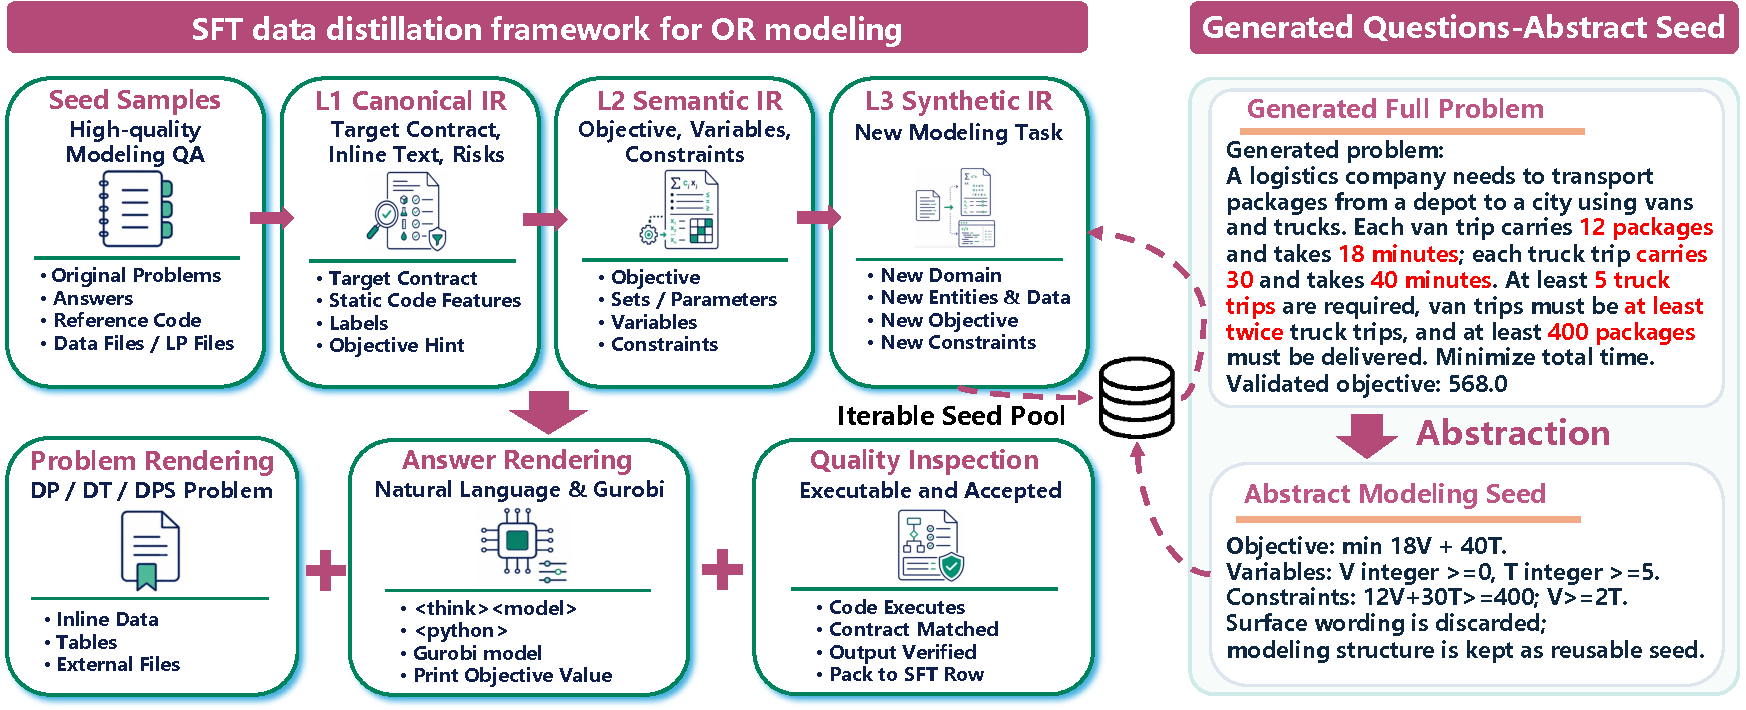
\includegraphics[width=\linewidth]{figures/flywheel.pdf}
% \caption{Overview of the SFT data distillation framework for OR modeling. The pipeline converts high-quality seed samples into canonical and semantic intermediate representations, generates novel synthetic IRs, renders them into multiple problem formats, validates the corresponding answers, and feeds accepted synthetic IRs back into the next self-distillation round.}
% \label{fig:sft_distillation_framework}
% \end{figure}

% \FloatBarrier

\subsubsection{Self-Distilled OR Modeling Data Flywheel}
\label{subsec:sft_dataset_construction}
\label{subsec:sft_ir_flywheel}

We construct a self-distillation data-production pipeline for operations research and mathematical programming tasks. The input is a set of seed samples, including original problems, reference answers, reference code, data files, or LP files from high-quality modeling QA data. These seed samples are not directly exported as final training data. Instead, they serve as references for problem types, modeling structures, and target response specifications.

% The seed samples are organized into three problem modes. DP, namely Data in Problem, means that the data is directly written in the problem statement. DT, namely Data in Table, means that the data is provided in a structured table such as a Markdown table. DPS, namely Data-Problem Separate, means that the problem statement and data files are separated, for example, \texttt{data.json}, \texttt{instance.json}, or CSV files.

The seed samples are organized into three input modes, as summarized in Table~\ref{tab:sft_problem_modes}.

\begin{table}[t]
\centering
\small
\caption{Problem modes used in self-distilled OR modeling data.}
\label{tab:sft_problem_modes}
\begin{tabular}{llp{0.58\linewidth}}
\toprule
Mode & Name & Description \\
\midrule
DP & Data in Problem & Data are directly written in the problem statement. \\
DT & Data in Table & Data are provided in a structured table, such as a Markdown table. \\
\multirow{2}{*}{DPS} & \multirow{2}{*}{Data-Problem Separate} & The problem statement and data files are separated, such as \texttt{data.json}, \texttt{instance.json}, or CSV files. \\
\bottomrule
\end{tabular}
\end{table}

To make the self-distillation process controllable and auditable, we introduce three levels of intermediate representations. This layered design follows progressive synthesis strategies in optimization data generation, where intermediate representations help control problem complexity and structural diversity~\citep{yang2025optibench,wu2025training}.
\begin{itemize}
    \item \textbf{L1 Canonical IR} normalizes heterogeneous samples and records the source path, target contract, data interface, reference-file status, static code features, risk labels, and objective-function hints.
    \item \textbf{L2 Semantic IR} extracts the mathematical-programming semantics of the seed sample, including the objective function, sets, parameters, variables, constraints, data interface, and potential modeling risks.
    \item \textbf{L3 Synthetic IR} generates a new modeling-task abstraction based on the L2 seed and the historical accepted synthetic pool. It must not copy the seed problem statement, answer, code, LP file, file name, path, exact numbers, or formulation. Instead, it varies the domain, entities, objective semantics, variable families, constraint families, parameter schema, numerical range, and data shape.
\end{itemize}

To further reduce the risk of data leakage, we apply leakage-control checks throughout the distillation process. Candidate synthetic samples are compared against held-out evaluation samples at multiple levels, including surface-level problem wording and abstract modeling structure. Semantic-similarity filtering is used to reject near-duplicate problem statements, while IR-level constraints prevent the reuse of the same objective semantics, constraint patterns, parameter schema, or numerical values. These controls ensure that the accepted SFT samples differ from the test set not only in textual expression, but also in data form and modeling structure, thereby reducing the possibility that the model learns leaked benchmark instances rather than generalizable OR modeling behaviors.

After L3 generation, the pipeline renders the synthetic IR into DP, DT, or DPS problems. DP samples embed data directly into the statement, DT samples contain structured Markdown tables, and DPS samples generate external files such as \texttt{data.json}, \texttt{instance.json}, or CSV files. The answer rendering stage then produces target responses according to the task-specific output contract. For Markdown-style answers, the response contains \texttt{<think>}, \texttt{<model>}, and \texttt{<python>} tags, while the Python code uses Gurobi to build and solve the model and output the objective value. In this way, the model learns not a single code template, but a family of modeling-output protocols under different task requirements.

The pipeline further adopts a flywheel-style iteration. Samples accepted into SFT in each round have their corresponding Synthetic IRs accumulated into the parent pool for the next generation round. The model therefore refers not only to the original Semantic IR, but also to previously accepted synthetic structures. This gradually reduces direct dependence on the original seeds and expands the modeling-structure space, while still using the seed data as anchors to prevent distributional drift. As illustrated in Figure~\ref{fig:sft_distillation_framework}, the overall framework connects seed samples, intermediate representations, problem rendering, answer rendering, automatic validation, and accepted-pool feedback.

\begin{figure}[t]
\centering
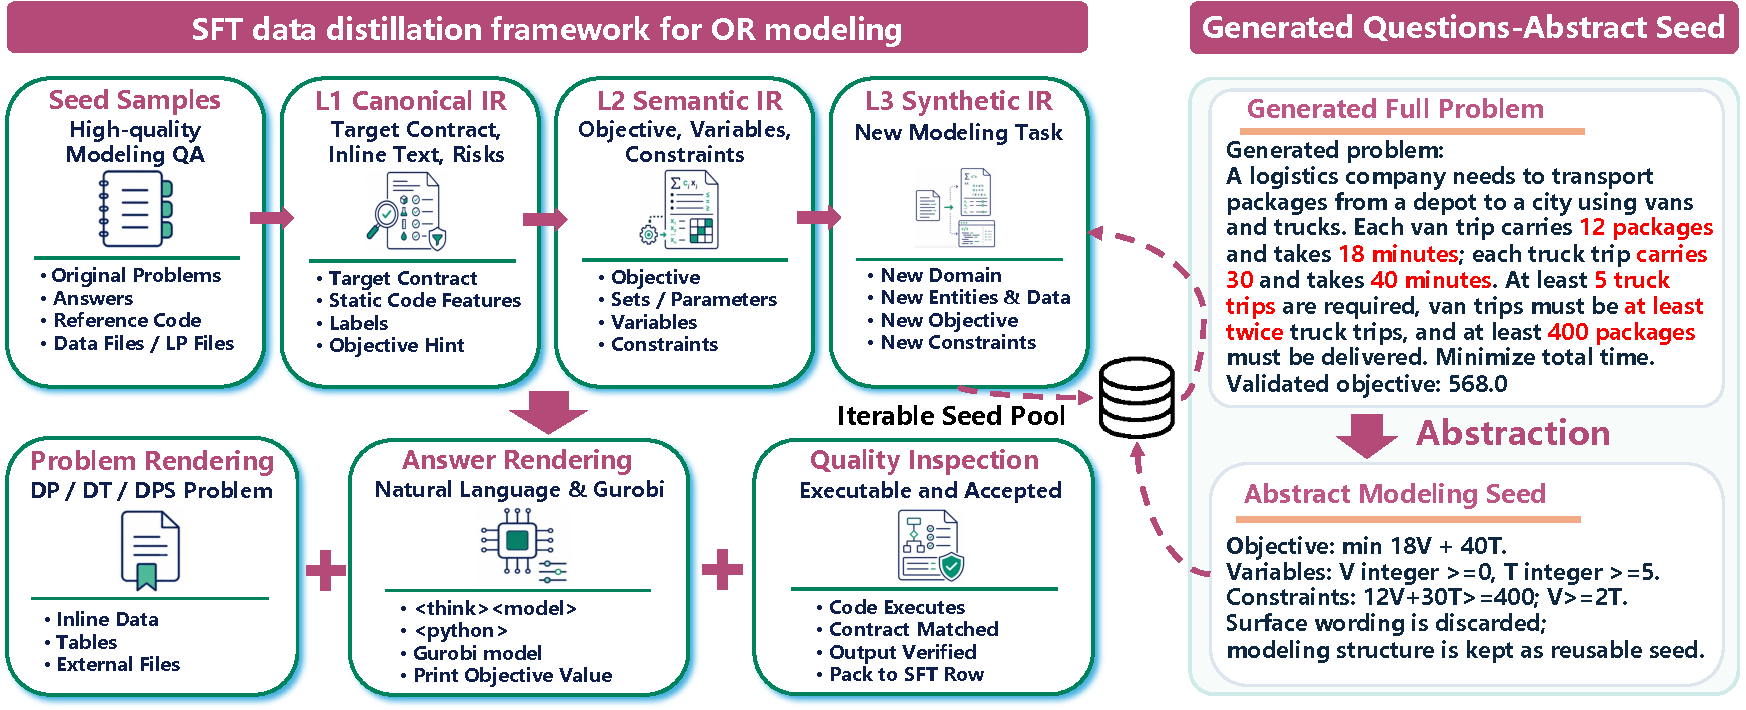
\includegraphics[width=\linewidth]{figures/flywheel.pdf}
\caption{Overview of the SFT data distillation framework for OR modeling. The pipeline converts high-quality seed samples into canonical and semantic intermediate representations, generates novel synthetic IRs, renders them into multiple problem formats, validates the corresponding answers, and feeds accepted synthetic IRs back into the next self-distillation round.}
\label{fig:sft_distillation_framework}
\end{figure}




% \subsection{Contract-Aware Cleaning and CoT Enhancement}
% \label{subsec:sft_cot_cleaning}

% The observations from preliminary SFT runs motivate a shift from merely enlarging the self-distilled dataset to improving the learnability of already distilled samples. In the comparison among 3K, 10K, and 50K reported in Section~\ref{subsec:sft_training_cleaning}, the 10K dataset already significantly improves Bench4Opt protocol-oriented tasks, but it remains below the baseline on NL4OPT and OptiBench. Further scaling to 50K does not recover this ability. Therefore, instead of continuing to expand the same pipeline to 100K, we perform fine-grained cleaning of the existing 10K data, focusing on modeling errors and chain-of-thought expression.

% The cleaning process first targets concrete error types exposed in the previous stage. In optimization modeling tasks, structural errors that directly damage the training signal include incorrect variable types, wrong objective direction, wrong constraint direction, missing capacity or demand constraints, improper handling of ratios or averages, and incorrect use of the Gurobi API. For example, objects such as counts, vehicles, routes, assignments, and selections are usually modeled as integer or binary variables, whereas continuous quantities such as tons, liters, flow rates, and working hours should not be over-integerized.

% In implementation, we design two cleaning branches. The first branch is \textbf{clean-only}, which aims to repair only real modeling or implementation errors while preserving the original reasoning style as much as possible. It does not actively add new explanatory content. The second branch is \textbf{clean-cot}, which repairs errors and also adds a concise modeling checklist into the target response. This checklist makes the \texttt{<think>} block explicitly cover variable types, objective direction, key constraints, ratio or nonlinear forms, and Gurobi execution actions. The goal of this chain-of-thought enhancement is not to generate long free-form reasoning. Instead, it compresses the original long-form problem understanding into a structured checklist. Supervised fine-tuning with Chain-of-Thought (CoT) reasoning has been shown to effectively transfer reasoning capabilities to LLMs~\citep{yu2025long}, and structured CoT data can facilitate more efficient reasoning without the overhead of unconstrained long-form generation~\citep{lin2025facilitating}. Recent work has also demonstrated that SFT with CoT data allows models to reach higher performance and facilitates easier subsequent improvements~\citep{yeo2025demystifying}. So that the model repeatedly observes a stable pattern: first determine variable domains, then determine the objective, then check constraints, and finally implement the formulation in Gurobi.

% The entire cleaning workflow uses four levels of gating: cleaner, reviewer, local validation, and export checking. The cleaner generates repaired candidate answers. The reviewer independently determines whether a candidate is suitable for SFT and blocks over-repair, such as incorrectly changing continuous variables into integers, deleting necessary constraints, or mishandling ratio and big-M formulations. Local validation then checks code executability, Gurobi calls, output contracts, and LP writing paths. In the full 10K run, clean-only passes reviewer filtering for 9,043 out of 10,000 samples, and 8,731 samples finally pass validation and are exported. Clean-cot passes reviewer filtering for 9,174 out of 10,000 samples, and 8,881 samples are finally exported.

% Overall, this cleaning stage is designed to make self-distilled SFT data more contract-aware and more learnable. For tagged Markdown targets, short structured \texttt{<think>} blocks inject the most error-prone optimization-modeling checkpoints into the training distribution. For code-only and LP-structure-equivalence tasks, the output contract remains strict, and later data construction should emphasize schema-to-code examples, error-repair pairs, and ORGEval-oriented structural-alignment data.

% \subsection{Two-Stage Progressive Fine-Tuning}

% Our scaling experiments reveal a fundamental conflict between the two capabilities that SFT must simultaneously instill: syntactic precision in solver-API usage and semantic reasoning in natural-language modeling. In a single-stage setup, gradient updates from pure code targets (e.g., Bench4Opt) and reasoning-rich targets (e.g., NL4OPT) interfere destructively, yielding the non-monotonic performance observed when scaling from 10K to 50K samples. To resolve this conflict, we decouple these capability dimensions into a two-stage progressive training strategy. The two-stage progressive paradigm has been shown to be more beneficial for domain adaptation, where continual pre-training on relevant corpora is followed by task-specific fine-tuning~\citep{zhang2024two}. This approach aligns with recent frameworks for domain-adaptive continued pre-training that separate general competence acquisition from specialized tuning~\citep{zhang2025adept}.

% Stage I, Solver-API Alignment, trains exclusively on code-only OR targets (LP-writing and feasibility tasks) with a conservative learning rate of \(5\times 10^{-7}\), establishing a stable, high-fidelity syntactic backbone for Gurobi invocations, data-loading patterns, and output contracts. Stage II, Full OR Modeling SFT, then continues from this checkpoint on the complete Clean-CoT 10K dataset with a higher learning rate of \(1\times 10^{-6}\), allowing the model to learn formulation and reasoning without contending with low-level syntax. This physical separation prevents the destructive gradient interference observed in monolithic training, preserving both syntactic robustness and reasoning fluency~\citep{yildiz2024investigating}.

% \subsection{General Capability Anchoring}

% The improvement in OR-specific tasks from SFT is accompanied by measurable degradation in general language understanding and code syntax health, as observed in our curriculum monitoring and the NL4OPT decline in Table~\ref{tab:main_results}. This drift toward domain specialization, while beneficial for solver-oriented benchmarks, erodes the general-purpose semantic representations that underpin natural-language modeling and agentic diversity. To counteract this forgetting, we augment the SFT mixture with \(10\%-15\%\) general-purpose instruction data (open-domain QA, multi-turn dialogue, and creative writing) interleaved with OR samples during Stage II training. This approach is motivated by findings in continual learning that domain-adaptive training must explicitly address the stability–plasticity trade-off to prevent catastrophic forgetting.

% This general-capability anchoring serves two purposes. First, it maintains a steady stream of gradient updates from diverse linguistic tasks, preventing the shared semantic representations from collapsing solely toward the solver-oriented distribution and thereby preserving NL4OPT performance. Second, by retaining broader lexical and structural diversity in the output distribution, the anchoring mitigates the parametric homogenization observed in our agentic rollout experiments, where SFT-induced updates suppressed persona-conditioned generation diversity. This ensures that the SFT checkpoint provides a more explorable initialization for the downstream agentic pipeline described in Section~\ref{sec:agent}.




\subsubsection{Contract-Aware Cleaning and CoT Enhancement}
\label{subsec:sft_cot_cleaning}

The observations from preliminary SFT runs motivate a shift from merely enlarging the self-distilled dataset to improving the learnability of already distilled samples. In the comparison among 3K, 10K, and 50K reported in Section~\ref{subsec:sft_training_cleaning}, the 10K dataset already significantly improves Bench4Opt protocol-oriented tasks, but it remains below the baseline on NL4OPT and OptiBench. Further scaling to 50K does not recover this ability. Therefore, instead of continuing to expand the same pipeline to 100K, we perform fine-grained cleaning of the existing 10K data, focusing on modeling errors and chain-of-thought expression.

The cleaning process targets concrete error types exposed in the previous stage. In optimization modeling tasks, structural errors that directly damage the training signal include incorrect variable types, wrong objective direction, wrong constraint direction, missing capacity or demand constraints, improper handling of ratios or averages, and incorrect use of the Gurobi API. For example, objects such as counts, vehicles, routes, assignments, and selections are usually modeled as integer or binary variables, whereas continuous quantities such as tons, liters, flow rates, and working hours should not be over-integerized.

We design two cleaning branches. The first branch is \textbf{clean-only}, which repairs real modeling or implementation errors while preserving the original reasoning style as much as possible. It does not actively add new explanatory content. The second branch is \textbf{Clean-CoT}, which repairs errors and adds a concise modeling checklist to the target response. This checklist makes the \texttt{<think>} block explicitly cover variable types, objective direction, key constraints, ratio or nonlinear forms, and Gurobi execution actions. The goal is not to generate long free-form reasoning, but to expose the model repeatedly to a stable modeling pattern: determine variable domains, determine the objective, check constraints, and implement the formulation in Gurobi. This design is consistent with recent findings that CoT-style SFT can transfer reasoning ability more effectively when the reasoning traces are structured and task-relevant~\citep{yu2025long,lin2025facilitating,yeo2025demystifying}.

The cleaning workflow uses four levels of gating: cleaner, reviewer, local validation, and export checking. The cleaner generates repaired candidate answers. The reviewer independently determines whether a candidate is suitable for SFT and blocks over-repair, such as incorrectly changing continuous variables into integers, deleting necessary constraints, or mishandling ratio and big-M formulations. Local validation then checks code executability, Gurobi calls, output contracts, and LP writing paths. In the full 10K run, clean-only passes reviewer filtering for 9,043 out of 10,000 samples, and 8,731 samples finally pass validation and are exported. Clean-CoT passes reviewer filtering for 9,174 out of 10,000 samples, and 8,881 samples are finally exported.

Overall, this cleaning stage makes self-distilled SFT data more contract-aware and more learnable. For tagged Markdown targets, short structured \texttt{<think>} blocks inject the most error-prone optimization-modeling checkpoints into the training distribution. For code-only and LP-structure-equivalence tasks, the output contract remains strict.

\subsubsection{Progressive SFT with General Capability Anchoring}

Our scaling experiments reveal a conflict between two capabilities that SFT must instill simultaneously: syntactic precision in solver-API usage and semantic reasoning in natural-language modeling. In a single-stage setup, gradient updates from pure code targets such as Bench4Opt and reasoning-rich targets such as NL4OPT may interfere destructively, leading to the non-monotonic performance observed when scaling from 10K to 50K samples. To reduce this conflict, we decouple these capability dimensions into a two-stage progressive training strategy. This follows the general idea of progressive domain adaptation, where broad task competence and specialized tuning are separated into different training stages~\citep{zhang2025adept}.

Stage I, \textbf{Solver-API Alignment}, trains exclusively on code-only OR targets, including LP-writing and feasibility tasks. It uses a conservative learning rate of \(5\times 10^{-7}\) to establish a stable syntactic backbone for Gurobi invocations, data-loading patterns, and output contracts. Stage II, \textbf{Full OR Modeling SFT}, continues from this checkpoint on the complete Clean-CoT 10K dataset with a learning rate of \(1\times 10^{-6}\). This allows the model to learn formulation and reasoning while preserving low-level solver syntax. By separating solver-API alignment from full modeling adaptation, the training process reduces the destructive interference observed in monolithic SFT~\citep{yildiz2024investigating}.

However, OR-specific SFT can still cause degradation in general language understanding and code syntax health, as observed in curriculum monitoring and the NL4OPT decline in Table~\ref{tab:main_results}. This drift toward domain specialization may erode the semantic representations needed for natural-language modeling and agentic diversity. To counteract this forgetting, we augment the Stage II mixture with \(10\%-15\%\) general-purpose instruction data, including open-domain QA, multi-turn dialogue, and creative writing. This general-capability anchoring maintains gradient updates from diverse linguistic tasks, helps preserve NL4OPT performance, and mitigates the parametric homogenization observed in agentic rollout experiments. As a result, the SFT checkpoint provides a more stable and explorable initialization for the downstream agentic pipeline.% described in Section~\ref{sec:agent}.










% 原chapter 5
\subsection{AI-Assisted Data Construction and Refinement}
\label{sec:ai}

\begin{figure}[t]
\centering
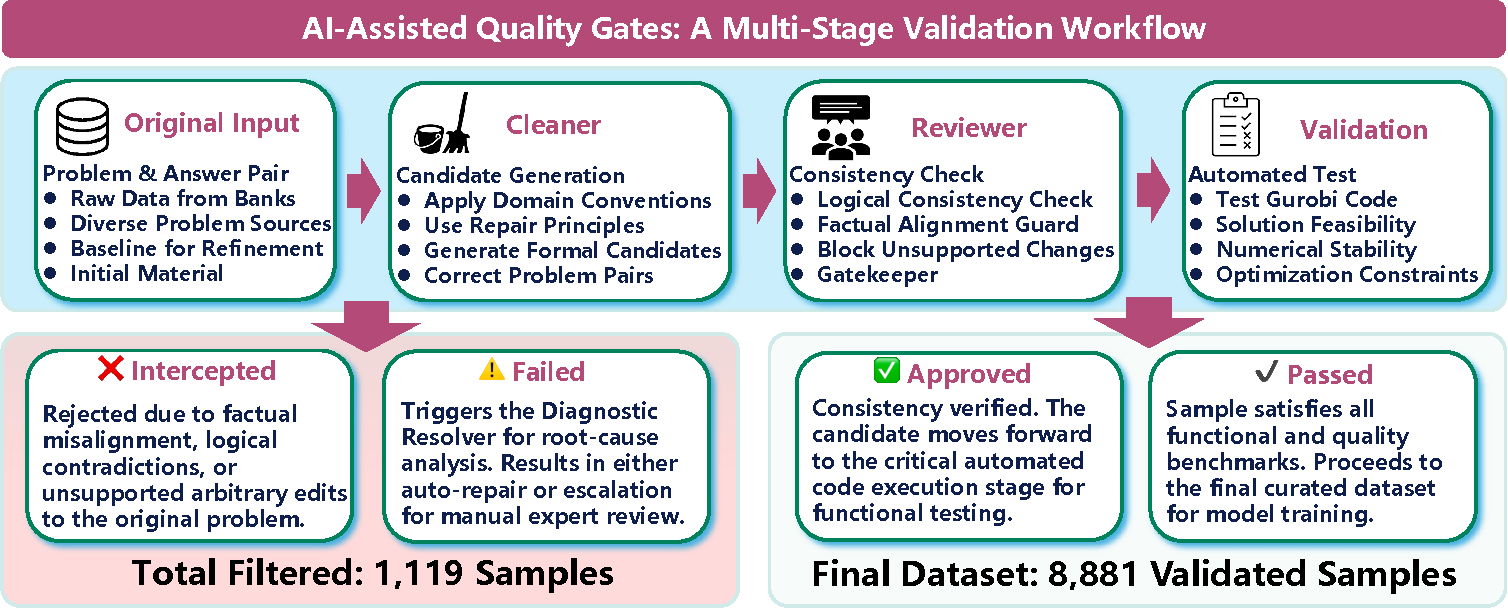
\includegraphics[width=\linewidth]{figures/ai_workflow.pdf}
\caption{The AI-Assisted Quality Gates workflow. This multi-stage validation process uses the Cleaner, Reviewer, and code execution Validation to ensure the quality and auditability of the final dataset.}
\label{fig:ai_workflow}
\end{figure}


To scale up the data construction process described above, we employ AI-assisted tools to automate candidate generation, repair, and validation. As illustrated in Figure~\ref{fig:ai_workflow}, the workflow combines an AI-based Cleaner and independent Reviewer with executable validation gates. Their tasks are inspired by multi-agent validation architectures~\citep{vallabhaneni2026ai}. In our workflow they operate as \textbf{prompt-and-rule-driven functions} under human-defined policies; no automatic rule invention is performed by the agents to ensure reproducibility. This section describes what these tools do and how they are orchestrated in our pipeline.

\begin{description}
    \item[Cleaner.] Given an original problem and answer, the Cleaner generates a repaired candidate. Its system prompt encodes the domain conventions, target contracts, and evidence-based repair principles described in the case studies. It is proactive in fixing clear errors (e.g., variable domain mismatches, missing constraints, obvious Gurobi API misuse) but can sometimes introduce new inconsistencies.

    \item[Reviewer.] The Reviewer evaluates each cleaned candidate independently, without access to the Cleaner's reasoning. It sees only the original problem, the original answer, and the cleaned answer. Its task is to check internal consistency and factual alignment with the prompt, and to block changes that are unsupported or introduce new errors. This adversarial check is essential to prevent over-repair.

    \item[Diagnostic Resolver.] When local validation (code execution against Gurobi) fails, the Resolver ingests the execution report, the problem statement, the current formulation, and the generated code. It produces a structured diagnosis attributing the failure to one or more categories: semantic modeling error, API usage error, data schema mismatch, or solver-incompatible expression. This diagnosis can trigger a second-stage repair or flag the sample for manual review.
\end{description}

The importance of the independent Reviewer is illustrated by an incident during development. For a transportation problem, the Cleaner accepted the sample with high confidence (\texttt{confidence = 0.95}) and reported only formatting changes. However, inspection of the cleaned output revealed that the cost from Warehouse~2 to Store~3 had been inadvertently changed from~2 to~3 in the \texttt{<model>} description, while the Python code correctly used~2. The Reviewer detected this inconsistency (\texttt{decision = needs\_repair}, \texttt{confidence = 0.95}) with the diagnosis: \texttt{issues = ["data\_inconsistency"]}. Without this gate, the conflicting sample would have entered SFT.

Across the full Clean-CoT run of 10,000 samples, the Reviewer intercepted 826 samples that the Cleaner had accepted; subsequent local validation caught an additional 293 samples. The final exported 8,881 samples are thus the intersection of three independent quality checks: Cleaner generation, Reviewer approval, and Validator execution. This multi-stage quality architecture is purely rule-driven and audit-trailed: every sample in the final SFT set carries verifiable history.

% ============================================================

% \section{Agentic Rollout Pipeline for OR Modeling}
% \label{sec:agent}

% Reinforcement learning with verifiable rewards has emerged as an
% effective post-training paradigm for LLMs, producing strong gains in
% single-turn reasoning tasks where execution or answer checking provides
% an automatic correctness signal~\citep{deepseekai2026deepseekr1incentivizingreasoningcapability, deepseekmath}~\citep{zeng2025reinforcing}. Extending this
% to agentic, multi-turn settings introduces a further challenge: a single
% outcome signal at the end of a long trajectory cannot easily assign
% credit to the intermediate steps that determined the outcome.
% General agentic RL frameworks such as RAGEN~\citep{ragen} and
% Search-R1~\citep{searchr1} address the multi-turn rollout challenge, but
% retain an outcome-level reward and leave credit assignment to individual
% stages as an open problem. We therefore design our pipeline around reward granularity rather than
% pipeline complexity, with each stage boundary chosen to produce an
% intermediate signal that the RL training loop can act on directly.

% OR modeling introduces two constraints that make outcome-level reward
% particularly insufficient. The first is the wrong-but-optimal failure
% mode: a formulation with a subtly incorrect objective or a missing
% constraint may still yield a feasible \texttt{OPTIMAL} solution, making
% the outcome reward positive and leaving the flawed trajectory without a
% corrective update. The second is the formulation--implementation
% attribution problem: when the outcome is wrong, a binary failure signal
% cannot determine whether the root cause lies in the mathematical
% formulation or in the code that implements it, so credit cannot be
% assigned to the responsible stage. OR-R1~\citep{orr1} demonstrates that
% outcome-level RL improves OR modeling, but treats the generation pipeline
% as a black box and does not address either constraint.

% Prompt-based OR pipelines such as OptiMUS~\citep{optimus2024},
% OR-LLM-Agent~\citep{zhang2025orllmagent}, and
% Chain-of-Experts~\citep{xiao2024coe} were designed for inference
% performance rather than RL training. Their stage boundaries are organized
% around solving the problem at inference time, not around exposing
% intermediate signals that function as rewards. Using such a pipeline as a
% rollout generator without modifying its stage structure leaves the reward
% coarse, the intermediate stages unobservable to the reward function, and
% the wrong-but-optimal failure mode unaddressed.

% Our pipeline is designed from the ground up as an RL rollout structure,
% with stage boundaries chosen to expose intermediate reward signals suited
% to the OR-specific error taxonomy. Stage~1 persona-based candidate
% sampling and Stage~2 consolidation produce structural diversity in the
% formulation space and synthesize it into a single candidate. Stage~3
% self-review checks the formulation before any code is generated and
% produces a structured verdict designed to serve as a reward signal for
% the formulation stages, independent of the final execution outcome and
% therefore applicable to the wrong-but-optimal failure mode that
% execution-based signals cannot reach. Stage~4 code generation and repair
% accompanies each failed attempt with a diagnosis that attributes the
% failure to either a formulation error or a code error, enabling
% differential credit assignment between the upstream modeling stages and
% the downstream implementation stage. Together, Stage~3 and Stage~4 are
% intended to supplement the single terminal outcome signal with a reward
% structure that directly addresses both OR-specific constraints.
% Each completed rollout produces a structured trajectory record
% consumable by the veRL training framework. We evaluate the pipeline in
% inference mode to characterize the failure modes that RL training is
% intended to address; the results are reported in
% Section~\ref{sec:experiment}. On-policy RL training is deferred to
% future work, as integration between veRL and the Ascend cluster remains
% under development.

% \begin{figure}[t]
%   \centering
%   \includegraphics[width=\linewidth]{figures/agent_pipeline}
%   \caption{Four-stage agentic rollout pipeline.}
%   \label{fig:pipeline}
% \end{figure}

% \subsection{Rollout Architecture}
% \label{subsec:agent_rollout}

% The rollout proceeds in four stages, as illustrated in
% Figure~\ref{fig:pipeline}. The ground-truth objective value is never
% exposed to the model at any stage; correctness is determined post-hoc
% by executing the generated code against Gurobi and comparing
% \texttt{model.ObjVal} to the reference value.

% \paragraph{Stage 1: Candidate sampling.}
% A single forward pass risks committing early to an incorrect modeling
% strategy with no opportunity for self-correction. We sample $n$
% independent candidate formulations, each guided by a distinct persona
% prompt that steers the model toward a structurally different approach to
% the problem. Temperature variation alone tends to produce outputs that
% differ linguistically while converging on the same underlying modeling
% strategy; persona-based sampling instead encourages diversity at the
% level of modeling decisions, such as the choice of primary decision
% variable or the degree of formulation compactness. Each candidate
% reasons through the problem independently and produces a complete
% mathematical model without any executable code.

% \paragraph{Stage 2: Consolidation.}
% Rather than selecting the best candidate by an external criterion, the
% model compares the $n$ candidates and synthesizes a single consolidated
% formulation. Because different candidates tend to make different errors,
% reviewing them side by side exposes those errors more readily than any
% single candidate would in isolation. This stage converts independent
% sampling diversity into a joint formulation that improves on what any
% individual candidate achieves.

% \paragraph{Stage 3: Self-review.}
% Before code generation, a dedicated review step checks the consolidated
% formulation for correctness and completeness, covering the objective
% function, decision variables, constraints, and overall feasibility.
% This is the stage at which wrong-but-optimal errors must be caught:
% once code is generated, an incorrect formulation that still yields
% \texttt{OPTIMAL} status produces no corrective signal in the Stage~4
% repair loop and the error persists into the final answer. When issues
% are identified, the same call produces a corrected formulation for the
% next review round; the loop terminates early once no issues remain, and
% otherwise runs for at most $r$ rounds.

% \paragraph{Stage 4: Code generation and repair.}
% Given the verified formulation from Stage~3, the model generates
% executable Gurobi Python code, which is run against the solver. If
% \texttt{OPTIMAL} status is not reached, the model diagnoses the root
% cause by jointly examining the problem statement, the current
% formulation, the generated code, and the execution report. The diagnosis identifies whether the failure originates from a
% formulation error or a code implementation bug. Based on this
% attribution, the model either revises the formulation and generates
% new code, or retains the formulation and fixes only the implementation. The repair prompt includes the outcomes of up to three
% prior failed attempts, so each new attempt is informed by the full
% within-round failure history. The loop runs for at most $R$ rounds and
% terminates early upon reaching \texttt{OPTIMAL}.

% \subsection{Trajectory Collection and RL Training Interface}
% \label{subsec:agent_rl_future}

% Each completed rollout produces two categories of intermediate records.
% Stage~3 generates a structured verdict at each review round, recording
% whether the consolidated formulation was accepted or revised and the
% formulation in use at the time. Stage~4 generates a structured diagnosis for each failed repair
% attempt, attributing the failure to either a formulation error or a
% code implementation bug, and recording the formulation in use at
% that point.

% For on-policy RL, the reward interface connects the rollout directly to
% the veRL training loop: the model generates trajectories under its
% current parameters, each is scored, and parameter updates follow. The
% trajectory-level reward, determined by whether the final Stage~4 attempt reaches
% \texttt{OPTIMAL} with the correct objective value, serves as the
% ground-truth anchor for the full pipeline, since it is the only signal
% that reflects actual solver verification rather than the model's own
% intermediate assessment. The Stage~3 verdict and Stage~4 diagnosis
% records extend this with per-stage signals: the verdict provides a
% formulation-quality score independent of execution outcome, and the
% diagnosis enables differential credit assignment between the upstream
% modeling stages and the downstream implementation stage. Whether
% trajectory-level reward alone is sufficient, or whether per-stage
% rewards produce meaningfully better credit assignment, is a question we
% plan to investigate once RL training is operational.